% Stanford University undergraduate honors thesis style -- modifications to the report style
% This is unofficial so you should check with your department and advisor
% See http://library.stanford.edu/research/bibliography-management/latex-and-bibtex
% 
% Example of use below
% See the suthesis-ug.sty file for documentation
%
% !TEX root = ./main.tex

\documentclass[twoside]{report}
\usepackage{suthesis-ug}
\usepackage{graphicx}
\usepackage{apacite}
\usepackage{natbib}
\usepackage{indentfirst}
\usepackage{fontawesome5}
\usepackage{xcolor}
\usepackage[hidelinks]{hyperref}
\usepackage{caption}
\usepackage{subcaption}
\usepackage{booktabs}
\usepackage{enumitem}
\usepackage{amsfonts}

\usepackage{subcaption}
% \usepackage[title]{appendix}
\usepackage{float}
\usepackage{amsmath}
\usepackage{multirow}
\usepackage{graphics}
\usepackage{array}
\usepackage{tabularx}
\usepackage{scrextend}
\usepackage{blindtext}
\usepackage{hyperref}
\usepackage{bbm}
\usepackage[colorinlistoftodos]{todonotes}
\usepackage[%
%   final%
]{pdfcomment}

% \makeatletter
% \def\namedlabel#1#2{\begingroup
%     #2%
%     \def\@currentlabel{#2}%
%     \phantomsection\label{#1}\endgroup
% }
\newcommand{\usageitem}[1]{%
  \item[%
    {\makebox[2em]{\strut #1}}%
  ]
}

\hypersetup{colorlinks=false,
    linkbordercolor=red,
}
\setlength\parskip{\baselineskip}


\dept{School of Computer Science}
\begin{document}
\setstretch{1.3}
    \title{the Language of Sketches}
\author{Xiaoyu Zhang}
\principaladvisor{Oliver Kroemer}
\patitle{Assistant Professor}
\padept{Robotics Institute, School of Computer Science}
\coprincipaladvisor{Yonatan Bisk}
\copatitle{Assistant Professor}
\copadept{Language Technology Institute, School of Computer Science}

\beforepreface
\prefacesection{Abstract}
Creative AI has seen much progress in recent years. Works like DALL-E 2 can generate inspiring art pieces from text descriptions. Instead of synthesizing realistic art works from language, we approach creativity from a different angle and investigate composition of semantic parts and visual concepts in sketches. For example, people can draw a circle to represent the moon, a scoop of ice-cream, or the face of a cat. In a similar way, language descriptors can be composed to create new concepts. People can draw a large round cat face or a narrow oval cat face. 


In order to study this reuse of abstract concepts, we construct a dataset of language annotated sketches.  We examined current sketch datasets and found that they either lack language annotations or semantic part annotations. Therefore, we collect a dataset of 11,150 (sketch part, text) pairs for 572 face sketches and 787 angel sketches. 


To understand the limits of current vision-language models, we fine-tuned CLIP,  a model pre-trained with a contrastive objective on 400 million (image,text) pairs and can map (image,text) pairs into a joint vision-language embedding space. We observed that (1) CLIP cannot easily generalize to an unseen category on the task of pairing sketches with their descriptions even though similar shapes and descriptions have occurred in training; (2) through fine-tuning, average cosine distance has increased between a pair of descriptors used by annotators to differentiate two sketches. With insights gained about how language and sketches interact in the CLIP embedding space, our aim is to facilitate research into models that can generate sketches in a part-based manner satisfying descriptions given by users of the pictures they have on their minds. 

\prefacesection{Acknowledgements}
I first and foremost thank my advisors, Professor Oliver Kroemer and Professor Yonatan Bisk, for advising me on this project. I am very grateful that I had the opportunity to explore the creative sketching domain with them during my Master's. 
Through working with them on this project, I have learned how humans use language creatively to describe sketches, and I am excited about building systems that can interact seamlessly with humans in the future. I want to thank Professor Jean Oh for being on my committee. 

I also want to thank my lab mates in the IAM and COMEDY lab (the name \textit{COMEDY} was coined in April 2022 \faIcon{laugh-wink}). Thank you guys for testing the numerous beta versions of my data collection interface and providing feedback without which the official deployment would not have been as successful. 

I thank my parents for encouraging me to pursue research topics that I enjoy. Thank you guys for listening to all my crazy ideas. 
\afterpreface

\chapter{Introduction} \label{introductionChapter}
Creative AI, such as using deep learning models to generate paintings and music, has been a popular research domain. Since creative activities are representative of unique human intelligence, numerous works have attempted to replicate the creative process on machines.
For example, Pharmako-AI \citep{allado-mcdowell_okojie_2020} is a book co-written by K Allado-McDowell and GPT-3 \citep{gpt3} through exchanges between the human and the language model. 
Works like DALL-E, GLIDE, and DALL-E 2 tackle the problem of synthesizing images from short language descriptions, and these generative models have produced many imaginative and inspring art pieces \citep{dallePaper,glidePaper,dalle2Paper}.
These work are often motivated by the vision to create machines that can interact with people and augment human creativity.  
Our work is driven by a similar vision: how can we build systems that can be creative like humans so that AI agents and people can pariticpate in creative activities together and inspire each other. 

\begin{figure*}[!htb]
\centering
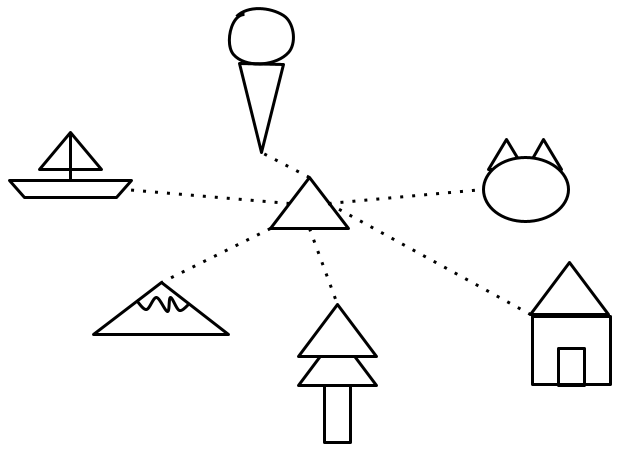
\includegraphics[width=.3\linewidth]{introduction/sketch_composition.png}  
\caption{Sketches of different objects with the triangle shape. The objects are, from top and in clockwise order: ice-cream, cat, house, pine tree, mountain, and boat.}
\label{introduction.composition}
\end{figure*}

Instead of studying how to generate realistic art works from a wide range of domains like DALL-E\todo[size=\small, color=green!20]{``a wide range of domain''?}, we approach creativity from a different angle and investigate composition of basic visual concepts to create different object sketches.
An example is illustrated in Figure \ref{introduction.composition}: a triangle can be a boat sail, a ice-cream cone, a cat ear, a house roof, a tree canopy, a mountain, etc. The same triangle is adapted to become different parts in sketches of different objects. 
While sketches do not contain all the details in natural images, they can still capture the essential features of different objects, making them simple yet widely recognizable. The abstractness allows for more creativity. 

In a similar way, language descriptors can be composed to form new concepts. For example, a \textit{large round} cat face versus a \textit{large squircle} cat face. The two faces share the same attribute \textit{large}, but one is more circular. Of course, cat face is not the only object that can be \textit{large round} or \textit{large squircle}; what object are you thinking right now that can have these attributes?
Moreover, a concept can be described in different ways. \textit{What visual features does this cat sketch have?} Some people might pick up on its usual size; others might notice its slightly edged chin, and there are still others that focus on the long whiskers curving upwards. People are likely to provide a variety of responses.  
% Word meanings shift depending on the context they are applied in. For example, the word \textit{large} in \textit{a large scoop of ice-cream} and \textit{a large cat face} implies size at different scales and conjure up different imagery. The \textit{large} scoop of ice-cream is probably oveflowing from the little cone underneath with the melting ice-cream dripping from the side, while the \textit{large} cat face implies a chubby round face compared to the cute pointy ears at the top.          

We want to build systems that can compose basic parts in a creative manner and understand how words are combined and adapted to describe different objects.  
In this thesis, we are interested in semantic parts in sketches and how people describe them. For example, a face sketch may contain four semantic parts: eyes, nose, mouth, and face contour, that can be drawn using various geometric shapes with different features.    

% % [B] 
% The ability to still get the idea across with such simple toolkit proves human creativity. We don't need complicated detailed realistic sketches, a few simple strokes are able to convey what we want to say. This type of creativity is innate. It is a creativity that we are born with: we start doodling as kids. We start scribbling on walls before knowing that we are re-creating our experience onto a canvas. It is the sort of creativity that lies on every one of us, and there is no high bar or artistic requirement to express this kind of creativity.

% % [B]
% Language creates space for imagination. Language creates room for creativity. The ambiguity in language. Large face. How large. Curved wings abstract away the details of the wings.

\chapter{Related Work} \label{relatedWorkChapter}

In this chapter, we survey two areas of related work: sketch datasets and sketch generation. 
There has been a proliferation of work on sketch representation learning \citep{ha2017neural,  eitz2012hdhso,spg_paper, qmulDataset, doodlerGAN, kim2019codraw, aksan2020cose, ribeiro2020sketchformer, Sketchpix2seqPaper, sketchBertPaper}. 
To study how human compose descriptors and shapes in sketches, we look into what annotations current sketch datasets contain and found that they lack either semantic part labels or language descriptions of the parts (Section \ref{related.sketch.datasets}).    
These datasets were created to solve classical computer vision tasks, such as recognition, segmentation, retrieval, whole-sketch generation, etc. 
We will then look into generative models of sketches in Section \ref{related.sketch.generate}. Although there have been many works on generating natural images, sketch generation has its own unique challenges: sketches contain sparse information and might bear little resemblance to their natural image counterparts; moreover, they illustrate features of the objects in an abstract way, such as a triangle as the house roof or a letter \textit{V} as the ice-cream cone. 
% DoodlerGAN is a recent work that looks into generating sketches in a part-based manner \citep{doodlerGAN}, closely related to our interests in studying how parts are combined in sketches. It follows a long line of works that employ generative adversarial networks (GAN) for image generation.  
% It also belongs to a set of works set of works on generating images from text descriptions or use texts to manipulate image styles, but they often work with a constraint set of language, with the exception of industrial-scale generative models with billions of parameters trained from text-image dataset on the hundred million scale      
% There is a long line of works on generating realistic images by learning their underlying distributions, especially on employing generative adversarial networks (GAN). 
% Related to our work is a .
%  
% Therefore, we also look into the field of sketch representation learning: what methods have been employed and what datasets are constructed.   

% \section{Image Synthesis from Text Prompts}


% \section{Sketch Representation Learning}

\section{Sketch Dataset} \label{related.sketch.datasets}
% Since our work seeks to collect a dataset of (sketch parts, text description), we survey existing sketch datasets and find that they either lack language descriptions, for the entire sketch or for parts in a sketch, or they do not contain semantic object annotations. 

\paragraph{TU-Berlin}
\citet{eitz2012hdhso} is one of the first works to investigate the characteristics of free-hand sketches and attempt to extract local features based on orientation, which are later used in the task of sketch recognition. 
It also provides the TU-Berlin sketch dataset that contains $20,000$ sketches spanning 250 object categories with 80 samples in each. 
The TU-Berlin dataset is then extended for sketch-based 3D object retrieval to contain 1814 new sketches for 130 common household object categories. This additional set also contains hierarchical category labels; for example, in the label hierarchy, the descendant categories of the \textit{animal} category are: \textit{arthropod, biped, human, flying creature, quadruped,} and \textit{underwater creature}. 
The TU-Berlin dataset contains some of the highest quality sketches for a wide range of categories, but they lack both text descriptions and semantic part annotations, and our dataset contains both types of annotations, although only for simpler sketches in the face and angel category.    

\paragraph{Datasets with Text Descriptions}
The QMUL dataset contains sketches of shoes and chairs: 419 shoe sketches of various types of shoes, such as high heels, boots, and ballerina flats, and 297 chair sketches of different kinds \citep{qmulDataset}. 
Although QMUL annotates for attributes of the sketches, they come from a fixed set of descriptions and are obtained from product tags, so these descriptions do not reflect how humans would creatively describe the drawings on their mind, which is a feature of our collected dataset.    
The Sketchy dataset contains $75,000$ sketches of 125 categories, and each sketch is paired with an image; Sketchy is additionally annotated with sketch validity metrics and short descriptions from annotators \citep{sketchyDataset}. However, these descriptions are more like comments given by the participants, and the collecting process is not carefully designed, unlike our data collection process, where obtaining the text description is the main focus. 
% ensuring the quality of the language
Moreover, the short texts in Sketchy do not describe individual semantic object in the sketches.     

\paragraph{QuickDraw Dataset}
The QuickDraw dataset is one of the largest sketch datasets, containing 50 million sketches distributed across 345 object categories. Each category has about 100,000 sketches \citep{ha2017neural}. 
Annotators for the TU-Berlin dataset have 30 minutes to draw one sketch, and annotators for the QMUL dataset have reference photos for the sketches they would draw later; on the other hand, participants of Quick,Draw! have 20 seconds to create the sketches for a randomly assigned category without time to look for reference, so sketches in the QuickDraw dataset are the simplest. However, since sketches that failed to be recognized by a classification model are filtered, they are in general of good quality and are representative of the general population drawing skills. Moreover, many works on sketch representation learning use the QuickDraw dataset, so utilizing these sketches would allow us to adapt other pre-trained generative models to model our dataset. 
These features of the QuickDraw dataset make it very favorable to be used to learn a collaborative drawing robot that can interact with a wide range of users, including children. However, the QuickDraw dataset contains neither semantic part annotation nor language descriptions, and our collected dataset contains both.   

\paragraph{Datasets with Semantic Part Annotations}
The sketches in our dataset come from the \\
QuickDraw dataset, but the original QuickDraw dataset does not provide labels for semantic objects in the sketches. 
The Sketch Perceptual Grouping (SPG) dataset \citep{spg_paper} and the SketchSeg dataset \citep{sketchsegDataset} contain annotations for semantic segmentation, meaning that each stroke in a sketch is paired with a semantic label. For example, strokes in a sketch for the \textit{face} category are assigned one of the following labels: \textit{eyes, nose, mouth, ear, hair, moustache, outline of face}. 
The SPG dataset annotates for $25,000$ QuickDraw sketches, belonging to 25 (out of 345) categories, and it selects 800 out of the original $100,000$ sketches in each category for annotation. 
The SketchSeg dataset builds upon the SPG dataset by using a recurrent neural work to generate additional sketches stemmed from one sketch in SPG; since each stroke in the generated sketch corresponds to a stroke in the original sketch, it automatically has part annotations. However, since the quality of the generated sketch is dependent upon the generative model, we choose the original SPG dataset, which is also publicly available. 
The SPG dataset does not contain text descriptions like our dataset, so we cannot study how people describe their sketches using SPG alone. 
% so although they can be used to build a collaborative drawing system, such system would not have the capacity to respond to natural language commands from users, and our work is interested in learning collaborative robots that can communicate freely with people.    
%DoodlerGAN

\paragraph{SketchCUB}
\cite{sketchbirds} collects a dataset, SketchCUB, of sketches and captions by transforming realistic images in the CUB dataset \citep{WahCUB_200_2011} into sketches with holistically-nested network (HED) \citep{hedPaper}. These sketches in the SketchCUB dataset are not done by humans and might not be representative of how the general population sketch, compared to those in QuickDraw.
The SketchCUB dataset contains 10K sketches over 200 different categories of birds. Moreover, the original CUB dataset collects the captions by presenting to the annotators a fixed set of attributes and asking them to determine whether the bird has the attribute or not. There are a total of 312 binary attributes, and they are traditionally used to determine species of birds in nature. Therefore, the captions might not represent how people describe sketch parts. 
The SketchCUB text descriptions are also for the whole sketch and not for individual semantic part in sketches.
In comparison, our dataset annotates for semantic parts in QuickDraw sketches, and we do not limit the annotators with a predefined list of words, so the descriptions tend to be more diverse and creative. There are a total of 1450 different words in our dataset.            
% 200 bird categories with 10,843 images. It includes a training set with 8,326 images in 150 categories and a test set with 2,517 images in the remaining 50 categories.  


\section{Sketch Generation} \label{related.sketch.generate}
%ShadowDraw

\paragraph{Sketch-RNN}
Along with the QuickDraw dataset, \cite{ha2017neural} introduces Sketch-RNN and provides a web demo of collaborative drawing, where users can select a category and draw the first few strokes of a sketch, and the model will complete the rest of the sketch\footnote{You can access the demo from this website \url{https://magenta.tensorflow.org/sketch-rnn-demo}}. Sketch-RNN uses a variational autoencoder (VAE) with bidirectional RNN encoder and RNN decoder. 

\cite{ha2017neural} uses a vector format to represent the sketches: each sketch is a set of strokes, and each stroke is a sequence of points, so the smooth curve is approximated with piecewise linear splines created by connecting adjacent points in the sequence. 
Works in sketch representation learning can be grouped into those that represent the input in this stroke-point vector format and those that treat the entire sketch as a raster image. 
Each point is a 5-component vector, $(\delta x, \delta y, p_1, p_2, p_3)$: the first two components represent changes in the $(x,y)$ coordinate of the current point compared to the last one; the last three make up a one-hot vector representing current state of the sketch. Let $s = \begin{bmatrix}p_1 & p_2 & p_3\end{bmatrix}$, if the current point will be connected with the next point, $s = \begin{bmatrix}1 & 0 & 0\end{bmatrix}$;
if the current point is the last point in the current stroke, so the pen is expected to be lifted next, then $s = \begin{bmatrix}0 & 1 & 0\end{bmatrix}$;
if the current point is the last point in the sketch, then $s = \begin{bmatrix}0 & 0 & 1\end{bmatrix}$.     
The RNN encoder takes this sequence as input and uses the final hidden state $h$ of the RNN to parameterize Gaussian distributions of size $N_z$, from which a latent random variable $z \in \mathbb{R}^{N_z}$ is sampled. 
The latent $z$ will be used to (1) initialize the hidden state $h_0$ of the RNN decoder and (2) be concatenated with the vector at each time step and fed as input into the decoder.  
The RNN decoder predicts parameters for distributions (Gaussian mixture model for sampling $\delta x, \delta y$ and categorical distribution for sampling $p_1,p_2,p_2$) at each time step from the hidden states of the RNN. 
Since the decoder works in an autoregressive manner, it can \textit{encode} the first few strokes provided by the users into a hidden vector, which is conditioned on for later steps to produce distributions of points that make up the rest of the sketch. 

Although our work uses the QuickDraw sketches, we render the vectors into raster images in order to use CLIP and its vision-language joint embeddings, since compared to Sketch-RNN, we need to incorporate text descriptions of the sketch parts.
It is challenging to align semantic information in text with distributions of the $x,y$ coordinates. While language gives high-level guidance on how strokes are organized on canvas to illustrate a particular concept, the coordinate information is too low level if directly used without an intermediate level of abstraction to aggregate these low-level sequence.    

\paragraph{DoodlerGAN} 
DoodlerGAN \citep{doodlerGAN} is a recent work on creative sketching and represents sketches as raster images. It uses Generative Adversarial Network (GAN) to model the sketches\footnote{Try the DoodlerGAN demo here: \url{http://doodlergan.cloudcv.org/}}. 
Compared to Sketch-RNN, which can only complete the missing parts of sketches once users are done with their parts, DoodlerGAN generates sketches using a part-based approach. In this way, users and the system can take multiple turns to create sketches. 

The part-based GAN has two networks: a part selector and a part generator. Given an incomplete sketch with some parts drawn (for example, a bird with its eyes and beak), the part selector determines what kind of part to draw next (for example, the bird wings). Then given the partial sketch and the category of the next part, the part generator produces a raster image of the part and its location on canvas. 
The part generator is a conditional GAN derived from StyleGAN2 \citep{styleGAN2Paper}, and it takes as input an image with number-of-parts$+1$ channels: one channel for each part and an additional channel for the whole partial sketch. The part selector uses the encoder of the part generator with an extra linear layer at the end as the classification head. 

While the part-based generation aspect of DoodlerGAN aligns with our goal to study composition of shapes in sketches, there is no language associated with each part, and the generation process is not guided by language supervision. As indicated by \cite{doodlerGAN}, compared to vector inputs, raster images can take better advantage of spatial structure of sketch parts. We believe that there is a shared abstractness in sketches and language, and we want to explore this aspect by first collecting a (semantic part, language description) dataset and then learning a part-based generative model from language.   

\paragraph{SketchBird}
Along with SketchCUB, \cite{sketchbirds} introduces a GAN-based model that generates sketches of birds from captions. The model architecture is based on AttnGAN \citep{attngan_paper}.
A bidirectional long short-term memory (Bi-LSTM) network is used as the text encoder, which is trained with image-text pairs while minimizing the Deep Attentional Multimodal Similarity Model (DAMSM) loss, proposed in AttnGAN. 
This loss is calculated based on attention-driven text-image matching score, which is the dot-product similarity between words in the caption and image subregions. 

Although SketchBird is one of the few works that look at sketch generation from language, it is limited by the dataset that it is trained and evaluated on: as explained earlier, the SketchCUB dataset does not contain human-drawn sketches, and the captions come from a list of predefined attributes. On the other hand, our work is morivated by how people can express high-level concepts, such as \textit{circular}, through a variety of language, \textit{round}, \textit{moon-shaped}, \textit{ringlike}, \textit{disk-shaped}, and how these type of free-form language can be composed and used to generate abstract sketches, similar to those in the QuickDraw dataset.     

% calculated between a word vector and a weighted sum of vectors of image regions. The weight comes from a matrix of size $T\times 289$ ($T =$ number words in the sentence, and $289 =$ number of image regions), contining using dot-product similarity between word in the sentence and subregion in the image. 

% In terms of exploring the multimodal sketch generation realm (text-to-sketch synthesis), a recent work is SketchBird \citep{sketchbirds}. This work, similar to ours, deal with the unique challenge of generating sketches from textual descriptions. They setup the task to mimic or as a counterpart to the classic text to image generation on the CUB dataset \citep{WahCUB_200_2011}. 
% This work is also representative of a line of work that is based on GAN, unique in the way that it is outputting sketches, closer to the domain that we are interested in.
% The line of text-to-image synthesis work begins with conditional GAN \citep{cGAN_text_image}, which also reports results on the CUB dataset. 
% One thing we are especially interested in is how these models are able to extract the text features, and how they fuse text features with image features. Moreover what loss is used to encourage the alignment between the image and text domain. 

% It seems like from quite a few papers, such as \cite{joyce-chai-zscl}, fuse the visual and textual space by combining the visual features using weights calculated by dot-similarity between the two modality, or vice versa to achieve cross attention. \cite{joyce-chai-zscl} uses a LSTM+GloVE setup for the unimodal text embeddings. 

% What are some other ways that we can extract visually informed text embeddings. 
% StyleGAN-NADA: CLIP Guided Domain Adaptation of Image Generators
% Of course, there are other techniques to generate images from texts, namely, leverage large pretrained model such as GPT-3. GPT-3 and DALL-E are particular nowadays for researchers to replicate on their own and try to query the immense feature space for creative art pieces. However, the abstract art style work is not our focus, and while creativity is an interesting future direction, we emphasize the collaborative aspect more than creativity. 



\chapter{Data Collection} \label{dataChapter}
% \section{Overview} \label{dataoverview}

% Imagine the following scenario (inspired by the YouTube channel:[]):
% Today we are going to draw a smiling ice-cream cone. Okay, we are going to first draw a curve as the top of a big scoop of ice-cream. Next, we will draw a sequence of connected U's to represent the bottom of the overflowing ice-cream. Lastly, we will draw a large upside-down triangle as the cone of our ice-cream.

% We want to realize this kind of interactions with a robot, as a companion, so we need to collect a dataset that can help us to get closer to this goal. In order to study this problem, we want to collect human sketches, so the first thing we did was designing an web interface.  
% The leading questions of the data collection process. Our goal is to collect a dataset so that we can learn a model that can interactively draw sketches with users. Therefore, we want to collect the drawing for a single step and a person's description of the drawing. Our design of the interface centers around some key questions: 
% \begin{enumerate}
%     \item \label{data_design_3} Ensure that the drawing responds to the prompt. The underlying assumption here is that the prompt itself will give us some signals in terms of where the objects in the images might be.  
%     \item \label{data_design_1} From the design side, enforce annotators to breaking the sketch generation process into steps. The worst scenarios is for the annotators to   
%     \item \label{data_design_2} How do we make sure that annotators are breaking the sketches they provide into reasonable steps? What we mean by reasonable here is the fact that there should be a good correspondence between some parts of the sketch and the language that is used to describe it. Although in our daily interactions, we might say something like ``we now draw this'' or ``we can do this'', but from a model learning perspective, or more so as a first step, we want there to be little ambiguity in our language and disallowing words like ``this''.     
%     % {\color{red} \faIcon{question}} How to make sure that users can do not go outside the step? How to make sure that users do not miss a step? How to make sure that users do not cram two steps together? How to make sure that they remember to annotate for a step and also give the accurate descriptions? 
% \end{enumerate}

% \setlist[enumerate,1]{leftmargin=12mm}
% \begin{enumerate}[itemsep=6pt,topsep=6pt]
%   \usageitem{\centering \faBook} \label{test_1} \textbf{Dictionary} is ...
%   \usageitem{\centering \large \faIcon{phone-square-alt}} \textbf{Mobile phones} are cool ...
% \end{enumerate}
% Reflects main requirement \ref{test_1}{\faBook}
To study the composition of visual concepts, we need to collect a sketch dataset that contain both semantic part and language annotations. We tested two ways of collecting such dataset. Initially, in order to create a dataset with creative composition of shapes, such as the use of triangle in different sketches illustrated in Figure \ref{introduction.composition}, we designed text prompts like \textit{happy angel} and asked annotators to draw sketches in response to the prompts while annotating each step in their drawings.  
After deployment of pilot, although we collected many creative sketches, we saw major problems related to misalignment between the drawn parts and the text descriptions. We explain this prompt-guided design and its associated problems in Section \ref{datav1}.    

After re-design, we leverage existing sketch datasets, QuickDraw and SPG (both explained in details in Section \ref{related.sketch.datasets}), to solve the problems of low-quality part and text annotations unusable for model learning.    
% while the second version asks the users to annotate existing sketches. The turning point happens after a pilot deployment of the first version, during which we identified several problems: (1) users take too long to complete one task, and it is outside our budge to collect an ample dataset; (2) users cannot separate the entire sketch into steps consistently, and the annotations either describe more or less than what was done in a single step.
In the new version, we present two sketches at a time to annotators, where the sketches contain semantic parts that are visually contrasting to aid annotators in coming up with creative descriptions. We walk through the process of designing this \textit{contrasting} interface in Section \ref{datav2}. After receiving satisfactory pilot results, we deployed this version full scale on Amazon Mechanical Turk (AMT); we present statistics of the dataset and explain how it allows us to study creative composition of abstract concepts in Section \ref{datasummary}. 

% The following sections will walk through each version and discuss the data collected using each version. The following sections will walk through each version and discuss how the design reflects or answers the above N criteria and what in reality happened that caused us to change the design.  

% Later, we discovered that by simply using existing sketches without asking for users to draw for the prompt would significantly reduce the data collection time, and it would also allow us to put aside DQ \ref{data_design_1}. 
% In general, if you think about it, classic collection tasks such as assigning label to images/texts or drawing segmentation box, the goal of the task is very clear, and it is easy to determine the quality of the work when you glance at it, or easy to verify. At the beginning, we found it very difficult to describe what should be drawn and what should not be drawn, or what can be written and what cannot be written. 

% The general trend of the data collection process is that we try to simplify the data collection interface and reduce the number of criteria that we need to satisfy, since each introduces a factor of uncertainty. 

% Since the beginning of data collection, we try to answer the question, what is a semantic part in sketches?   
% The end goal is to achieve the kind of interaction shown in the YouTube video \textit{How To Draw A Cute Ice Cream Cone}, and in it, the instructor oftens uses sentences in the form of ``Let's draw a \texttt{X} for \texttt{Y}'', where \texttt{X} describes the geometric features of the object \texttt{Y}. For example, ``Let's draw \textit{small connected U shapes} for the \textit{bottom of the ice-cream cone}.'' 
% Therefore, at first, we thought of decomposing the drawing process into a sequence of common geometric shapes, and the objects that they represent become the basic semantic units.   
% there should be a fixed set of primitive that the users could choose from, so learning the model becomes learning to parameterize, for example, the dimensions of the set of primitives. 
% Why was I so fixated on the primitives, because the abstractness of the icons is what interested me the most. 

% Functionality:
% \begin{itemize}
%     \item Draw the figure and the page will record the sequence 
%     \item User can replay its drawing sequence. The original idea was that users will first create the drawing, and then they can replay the sequence as they annotate for each step. 
% \end{itemize}

% In terms of the main task, I created a test version to confirm that the idea of the drawing board is sensible.

% Press \textit{Record}, Draw on the board, Press \textit{Stop} when done with drawing, \textit{Submit} the drawing if one is satisfied with the quality, \textit{Play} to revisit the drawing, \textit{Cancel} to start over. 

% What was the original motivation behind this functionality was that it will aid the annotators to review the drawing process and divide it into better steps. Responding to DQ \ref{data_design_1}. 

% We begin with a very crude version, and then we decide to add features that can allow us to realize the DQ \ref{data_design_1} and \ref{data_design_2}.

% The actual Version 0 has the following flow:
% There is a practice board, you can try to practice drawing so that the actual drawing submit has good quality and respond to the prompt (reflecting DQ \ref{data_design_3}). Then hit \textit{Ready to Record}, again baking the sequence into the design of the website will help us to enforce collecting a dataset of steps. Another purpose is to help the annotators decide beforehand what are the necessary primitives used in the process. 
% The entire research journey was very explorative, it sorted of started with a sense of \textit{oh, this question or aspect of how humans do things is interesting, I wish robot can do the same}. And what is that thing that I thought was interesting, it was how Rain and I were able to draw the icons and the interactions. 
% The first thing you will do is select a primitive from a list, and then you will draw the step that contains the primitives. Hit \textit{Next} to move on to drawing the next primitive. There are will be a little tag at the bottom showing what is the primitive that corresponds to the step that is drawn on the board. Repeat until finished and hit \textit{Done}. At the end, again, \textit{Play}, \textit{Submit}, or \textit{Cancel} to start over. 

% {\color{red} \faIcon{question}} Should we use primitive shapes for users to choose from? 
% The reason for considering this aspect is whether during generation we want to learn to change parameters of a fix set of shapes or generate un-constrained strokes. For the first option, we want users to compose a drawing with primitive shapes   
% In order to learn a more general model, we decided that we want to collect strokes instead of fixed primitive shapes, so we moved onto creating a table that accompanies the drawing board, where the user can choose to annotate each step they draw. 

% In Figure \ref{v0.design}. 

% \begin{figure*}[ht!]
% \begin{subfigure}{\textwidth}
%   \centering
%   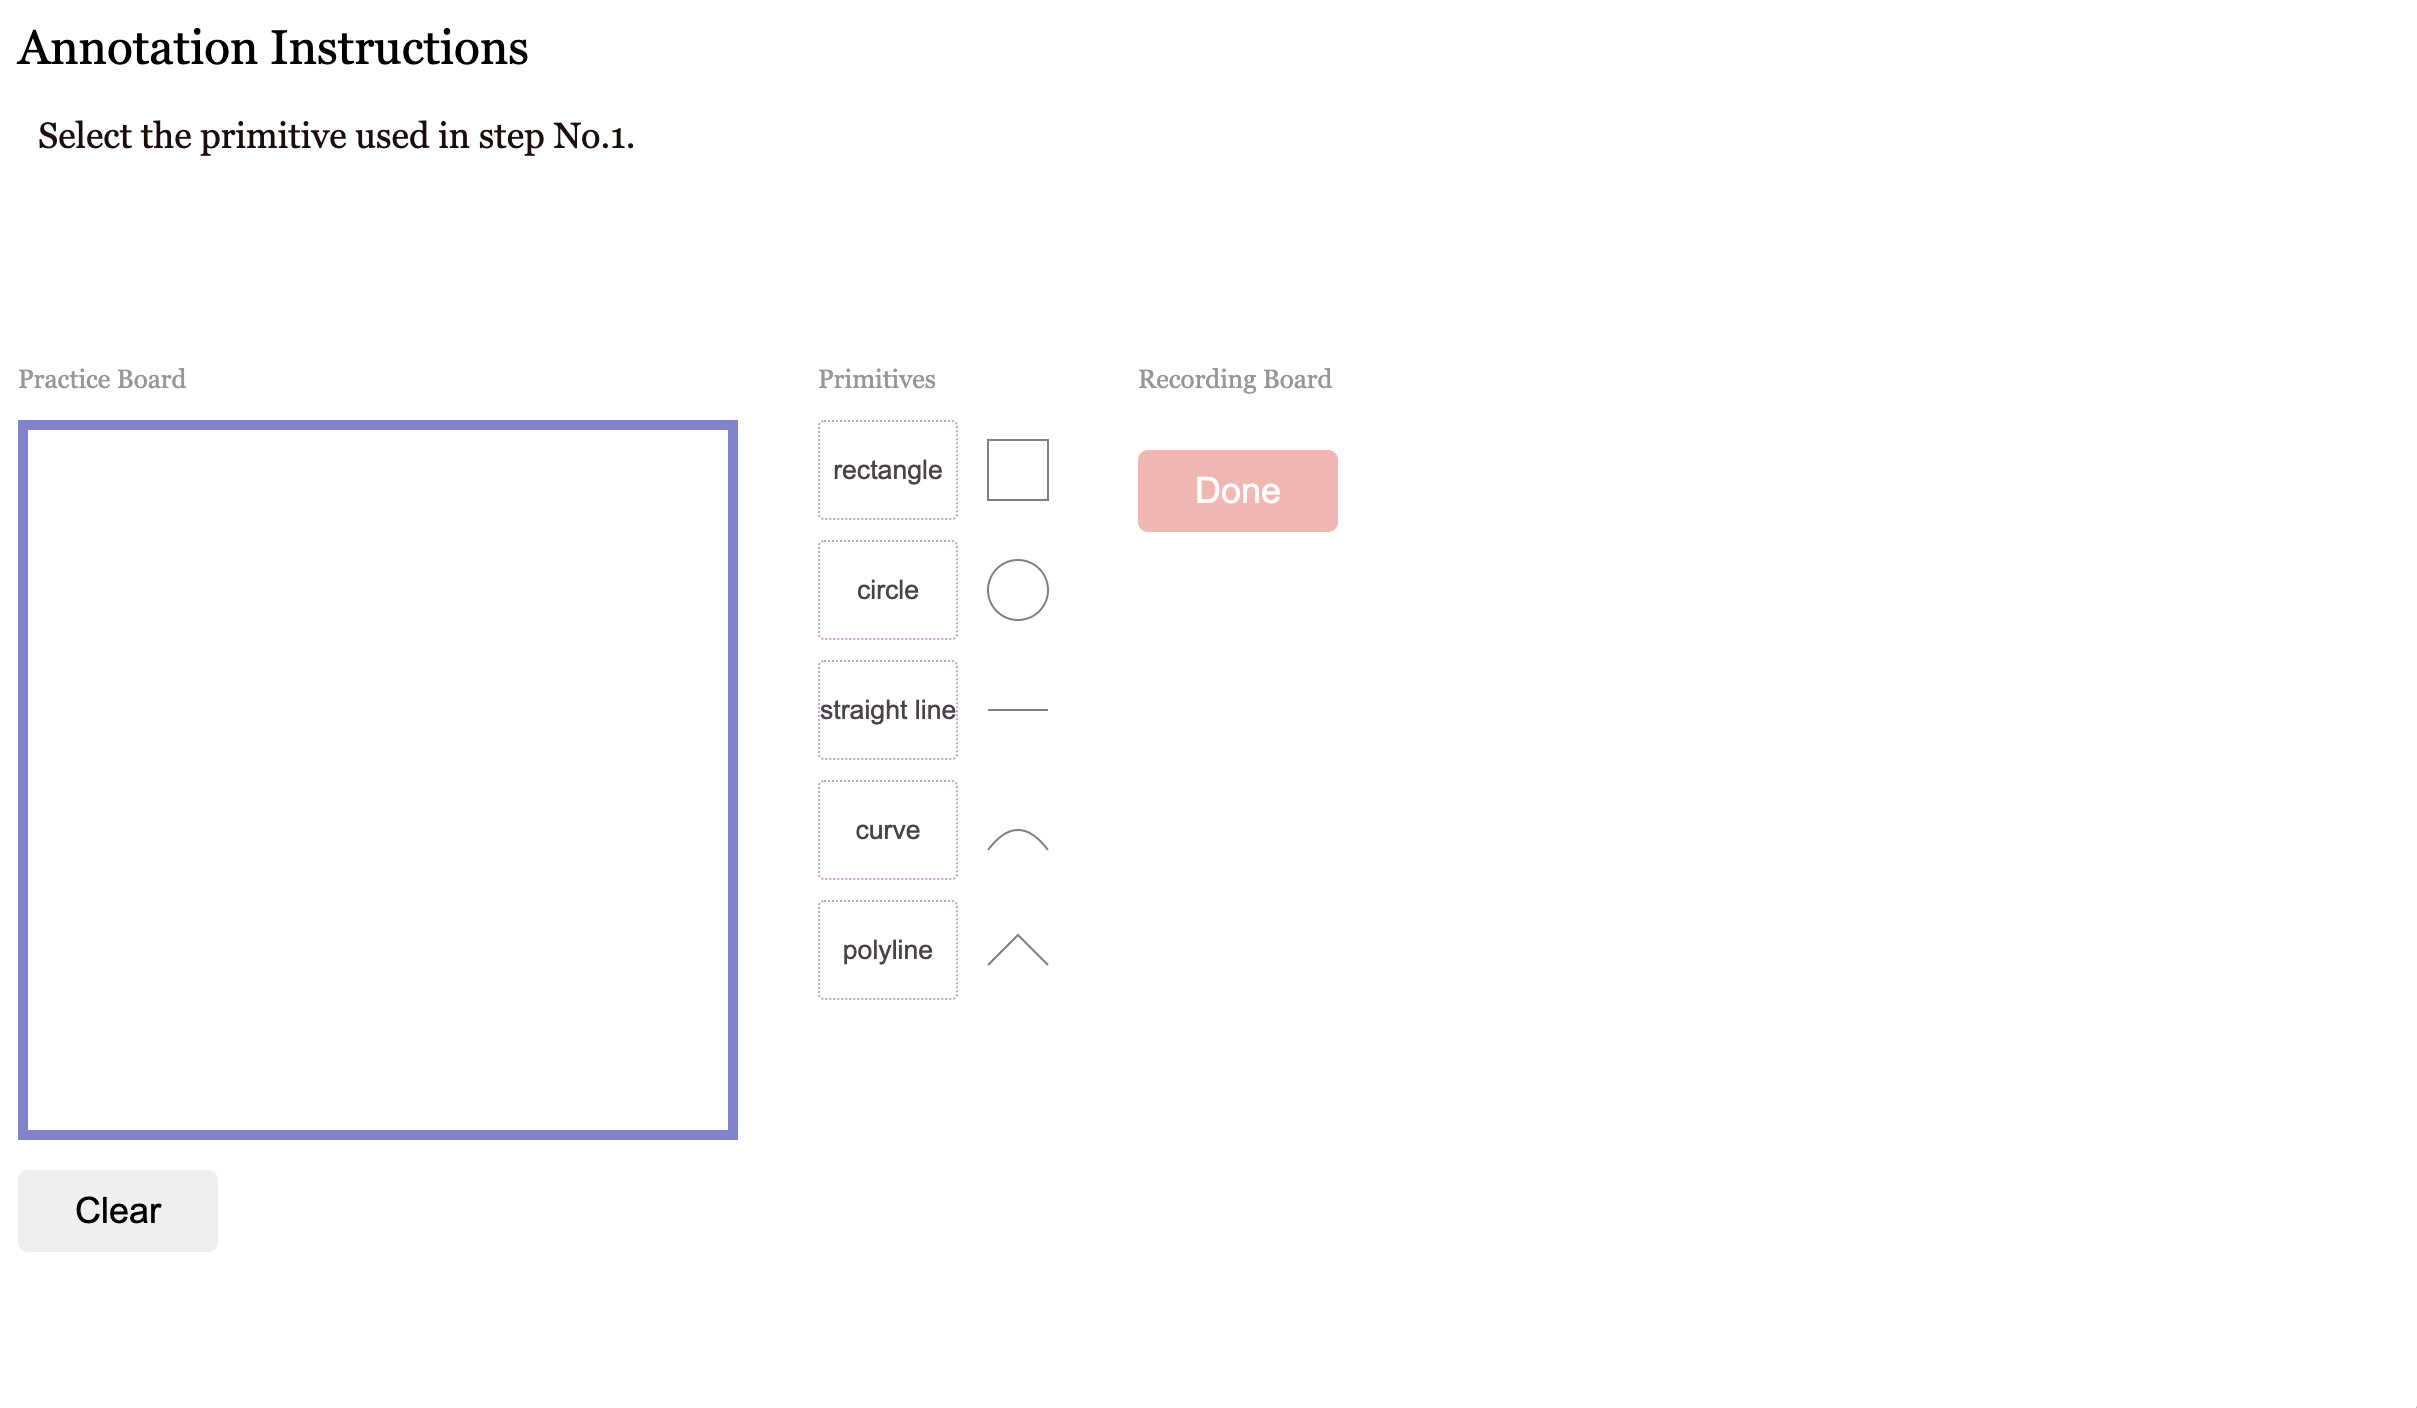
\includegraphics[width=.8\linewidth]{data_collection/version_0_select_primitive.png}
%   \caption{Design of main task for third pilot.}
%   \label{v0.1}
% \end{subfigure}
% \newline
% \begin{subfigure}{\textwidth}
%   \centering
%   % include third image
%   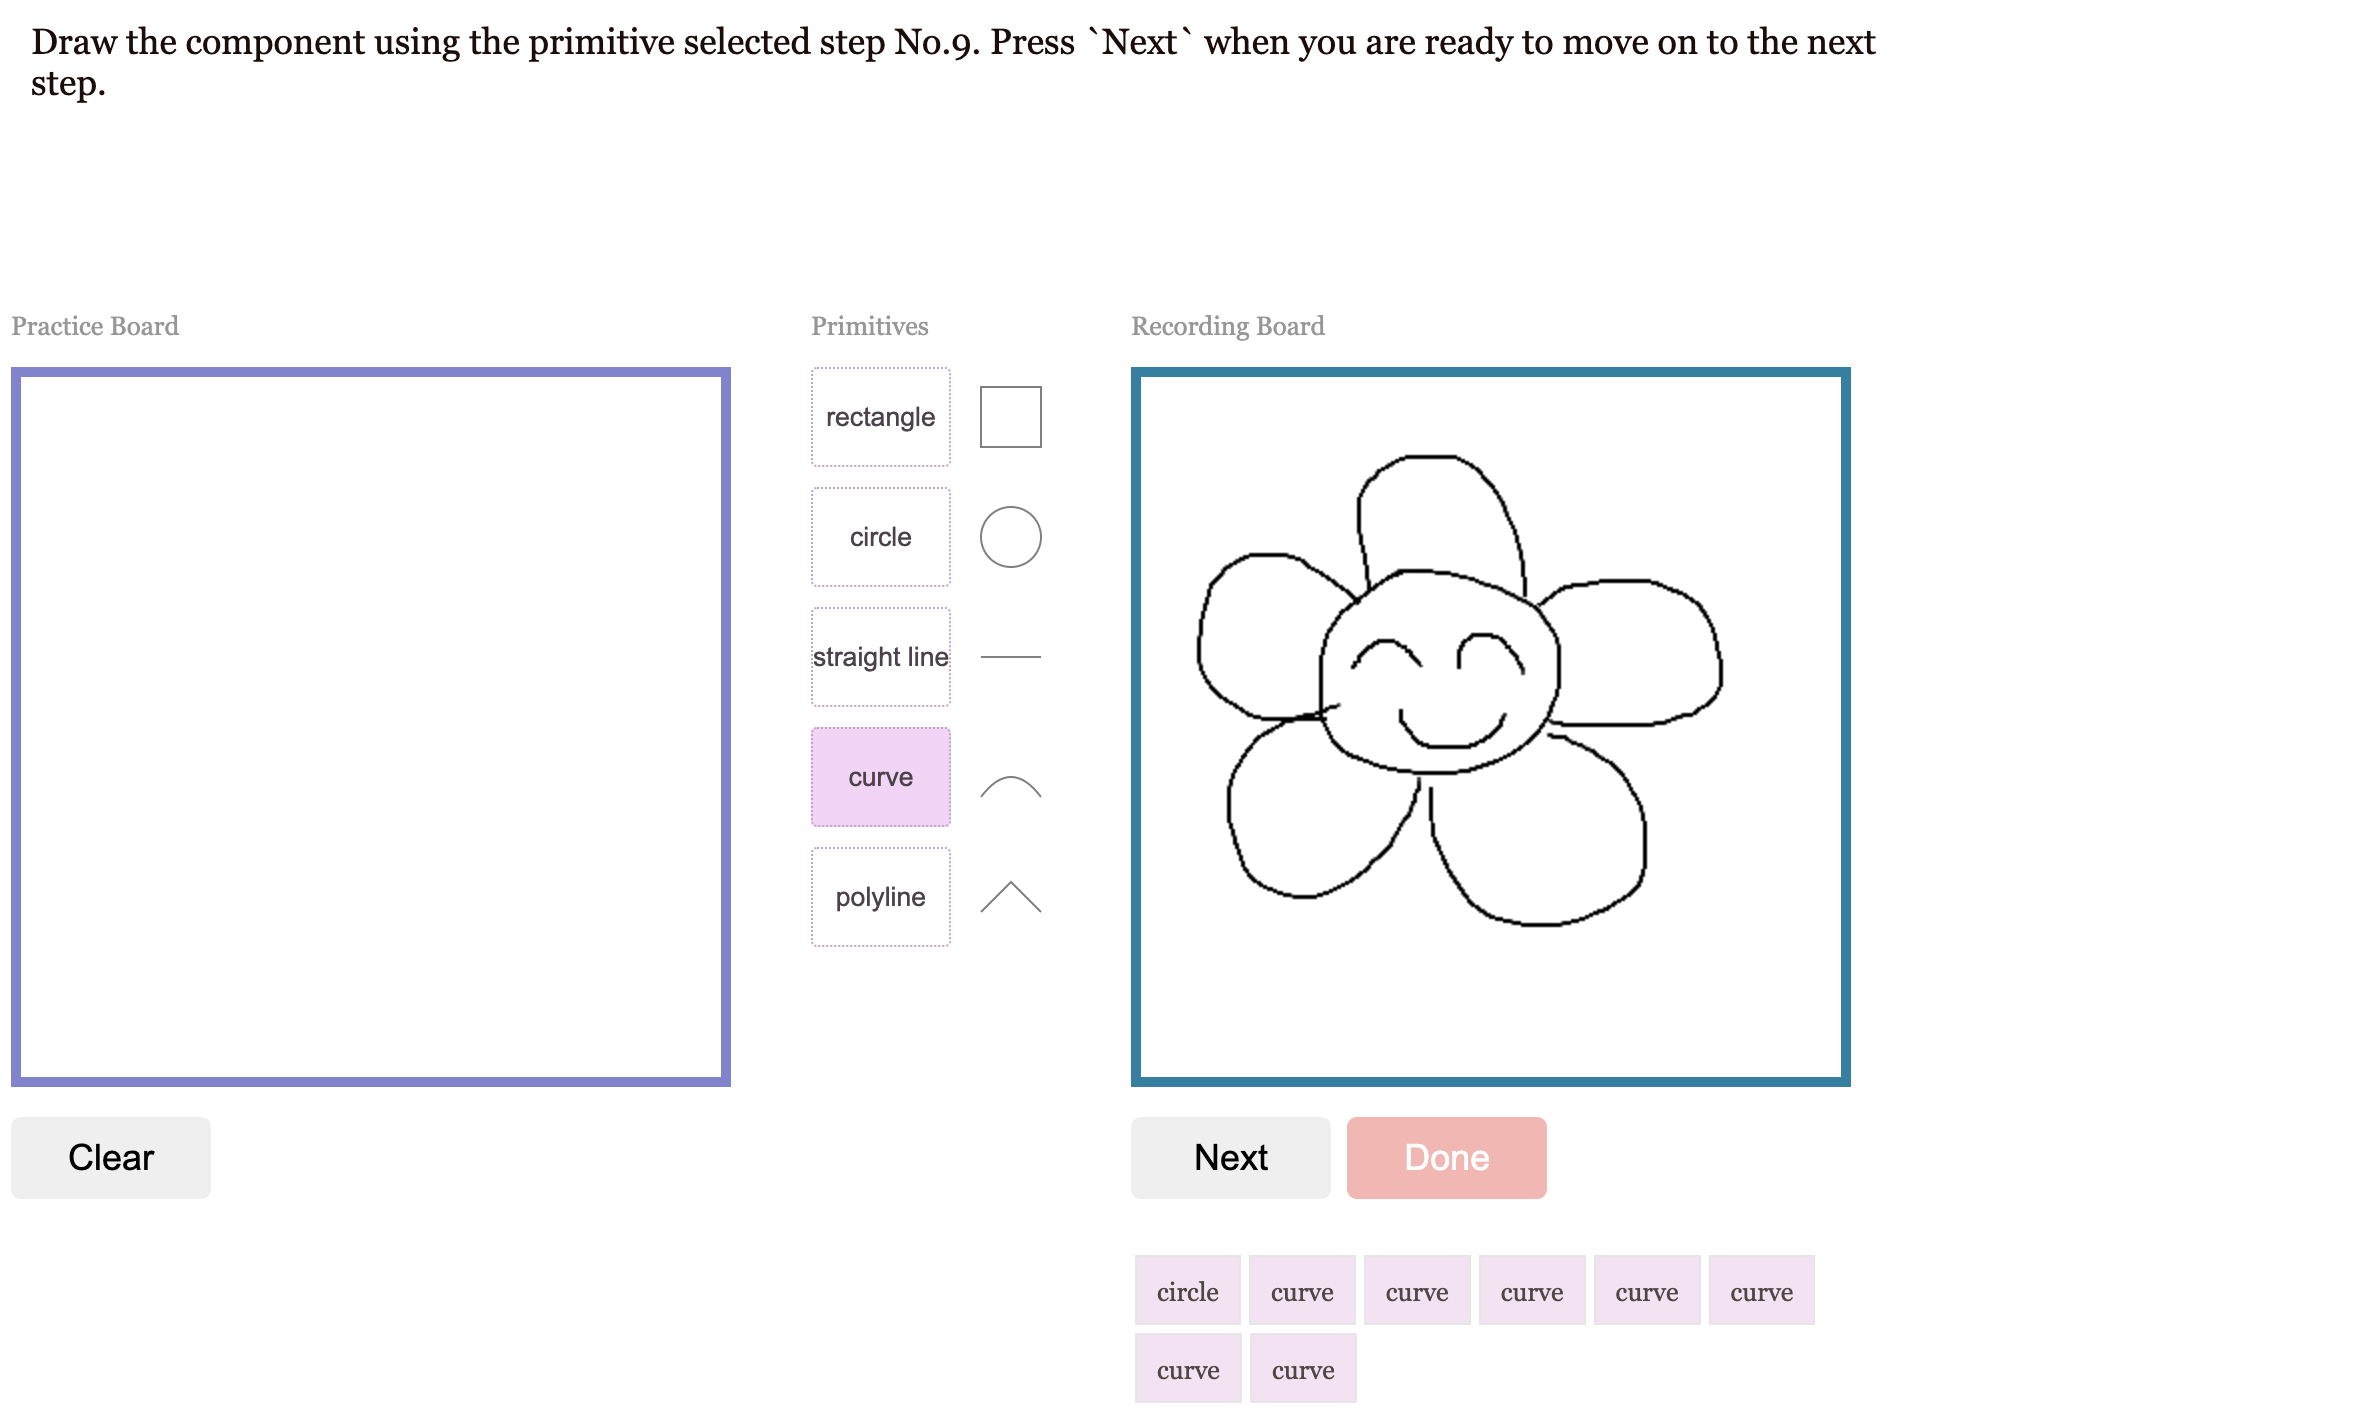
\includegraphics[width=.8\linewidth]{data_collection/version_0_smiley_flower_with_primitive.png}  
%   \caption{Design of main task for final task.}
%   \label{v0.2}
% \end{subfigure}
% \caption{Progress of the design two for the main task in version two.}
% \label{v0.design}
% \end{figure*}

\section{Prompt-Guided Sketch Text Dataset} \label{datav1}
\subsection{Overview}
When we first started designing our data collection interface, we wanted to collect sketches for prompts similar to the ones used in DALL-E \citep{dallePaper}: creative composition of attributes and objects that are not commonly associated with the attirbutes. For example, \textit{evil cup of bubble tea} and \textit{happy moon}. In addition to sketches, we also require annotators to decompose their drawings into steps and provide descriptions for each step. We hope to discover combination of simples shapes like examples in Figure \ref{introduction.composition}, and because the imaginative prompts would result in creative sketches, the part descriptions would also include unexpected usage of words.     

We deploy the data collection interface on Amazon Mechanical Turk (AMT), which is a crowd-sourcing website that hosts different machine learning annotation tasks. In the remaining text, we use the word \textit{turker} to refer to annotators we recruit on AMT; we will also use the word \textit{HIT}, Human Intelligence Task, to refer to a task hosted on AMT. Please refer to \href{https://www.mturk.com/worker/help#:~:text=A%20Human%20Intelligence%20Task%2C%20or,be%20completed%20by%20Worker%20customers.}{AMT FAQs} for official definition and answers to questions related to AMT. 
 
We have to design the following sections for the task: 
\begin{enumerate}
    \item \label{v1_sec_1} an interface containing the main task
    \item instructions and requirements to describe the tasks and specify what the annotators should and should not include in the annotations
    \item a qualification task accompanying the main task to train the turkers to produce high-quality annotations
\end{enumerate}
% Compared to Version 0, which we only dabbled with \ref{v1_sec_1} in the above list, we went through all three stages for Version 1 and eventually deployed a pilot.
After deployment, we realized that a few major problems from this design: (1) due to the subjective nature of drawing, it was hard to understand in what ways some annotators are illustrating the given prompts, thus making it difficult to determine the quality of the annotations; (2) turkers are taking more than 30 minutes for each task, showing that providing both sketches and descriptions are inefficient; (3) some turkers are unable to provide descriptions that align with the objects they meant to annotate for; for example, in one step, they drew both eyes and hair, but they only annotate ``big eyes''.      

\subsection{Interface Design}

\subsubsection{Main Task}
Compare to version 0, we make the following changes to the task interface: 
\begin{enumerate}
    \item Since turkers are paid based on time spent on the task, we decided to forsake the functionality related to the recording and replaying the drawing board.
    \item Since we decide to not limit the drawings to be compositions of basic geometric objects, we removed the step to select primitive shape preceding drawing each component.
\end{enumerate}

\begin{figure*}[!htb]
\begin{subfigure}{\textwidth}
    \centering
    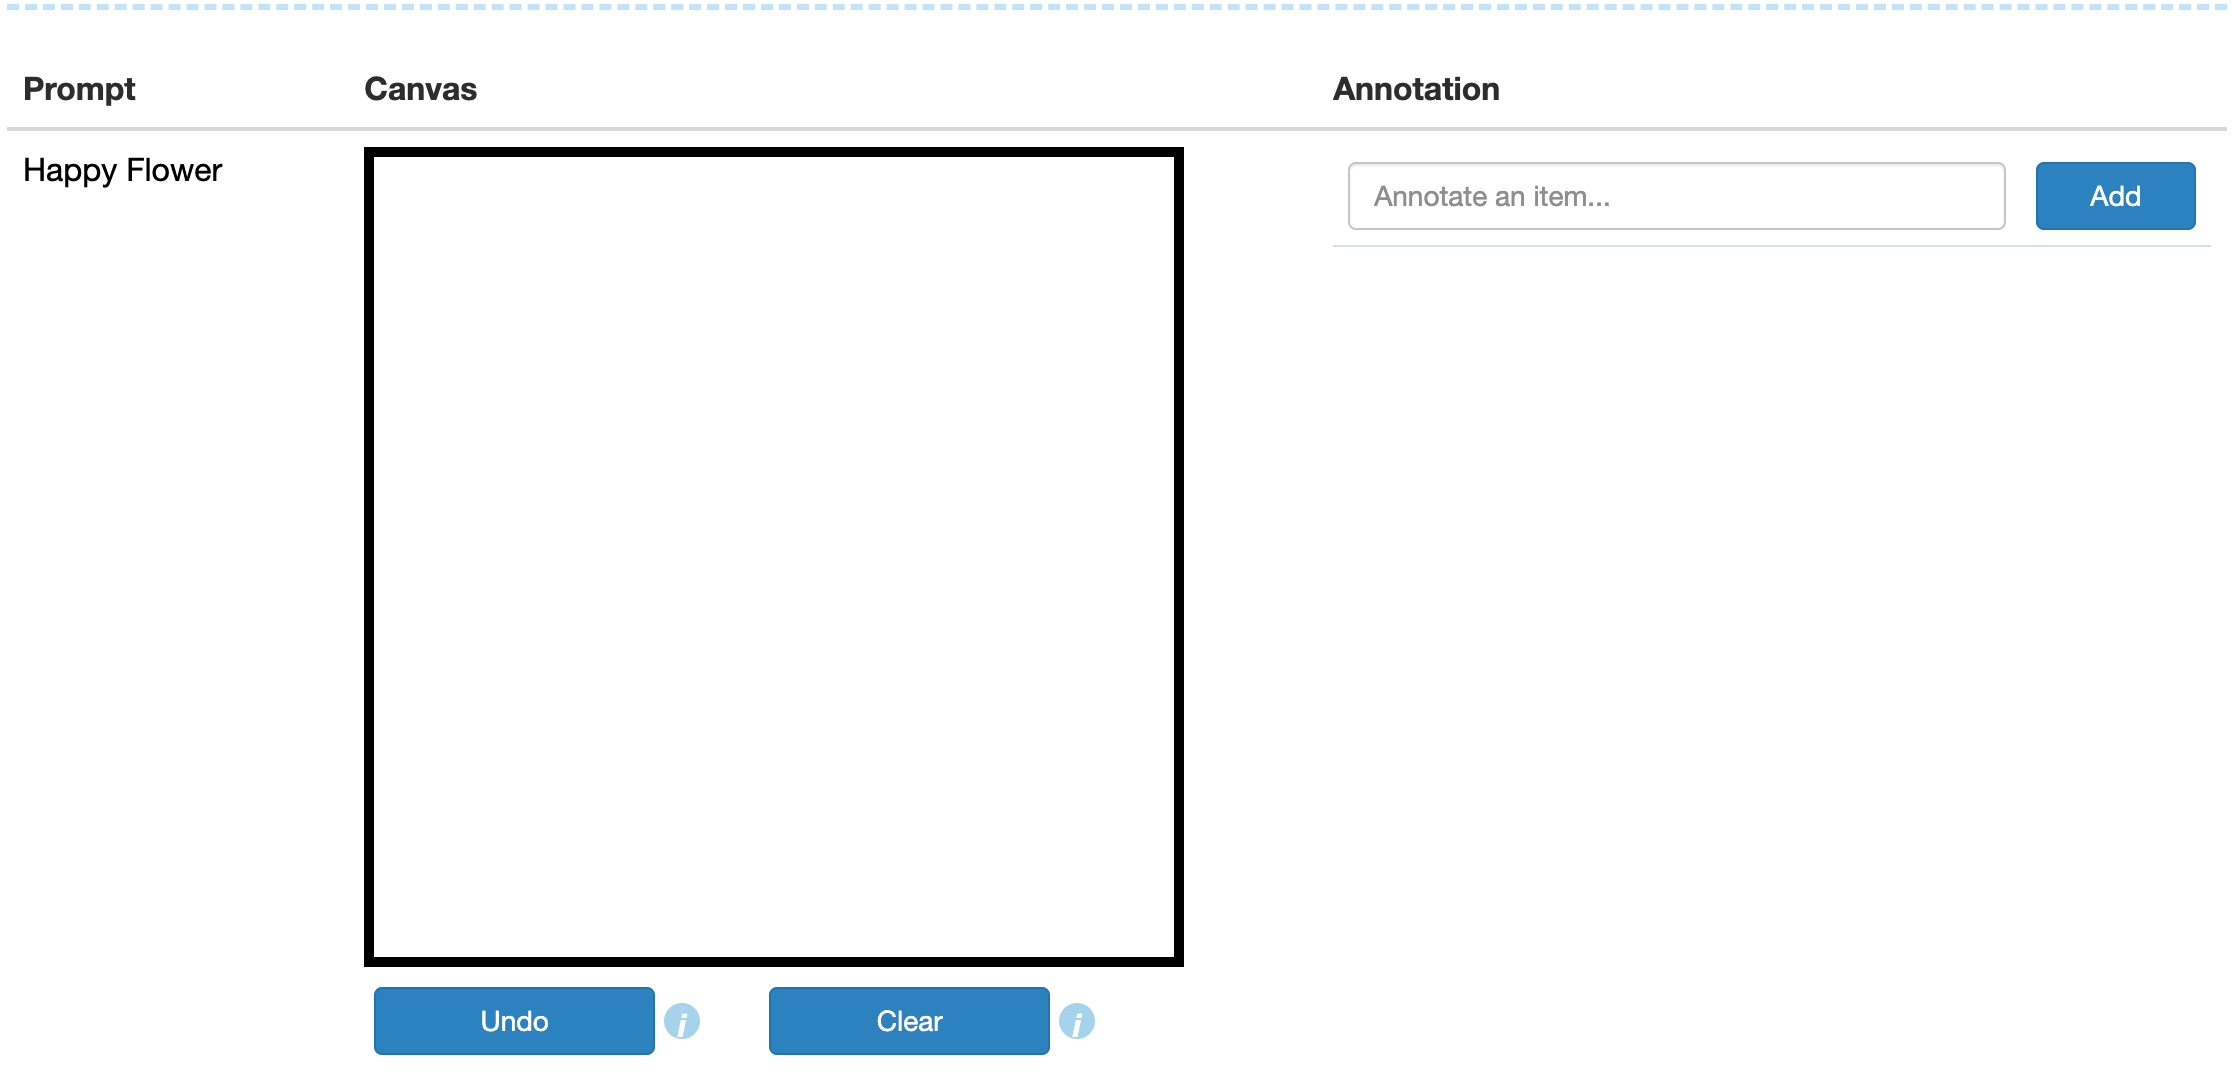
\includegraphics[width=.8\linewidth]{data_collection/v1_empty_table.png}  
    \caption{Main task interface at the start of annotation.}
    \label{v1.main_task.1.a}
\end{subfigure}
\newline
\begin{subfigure}{\textwidth}
    \centering
    % include third image
    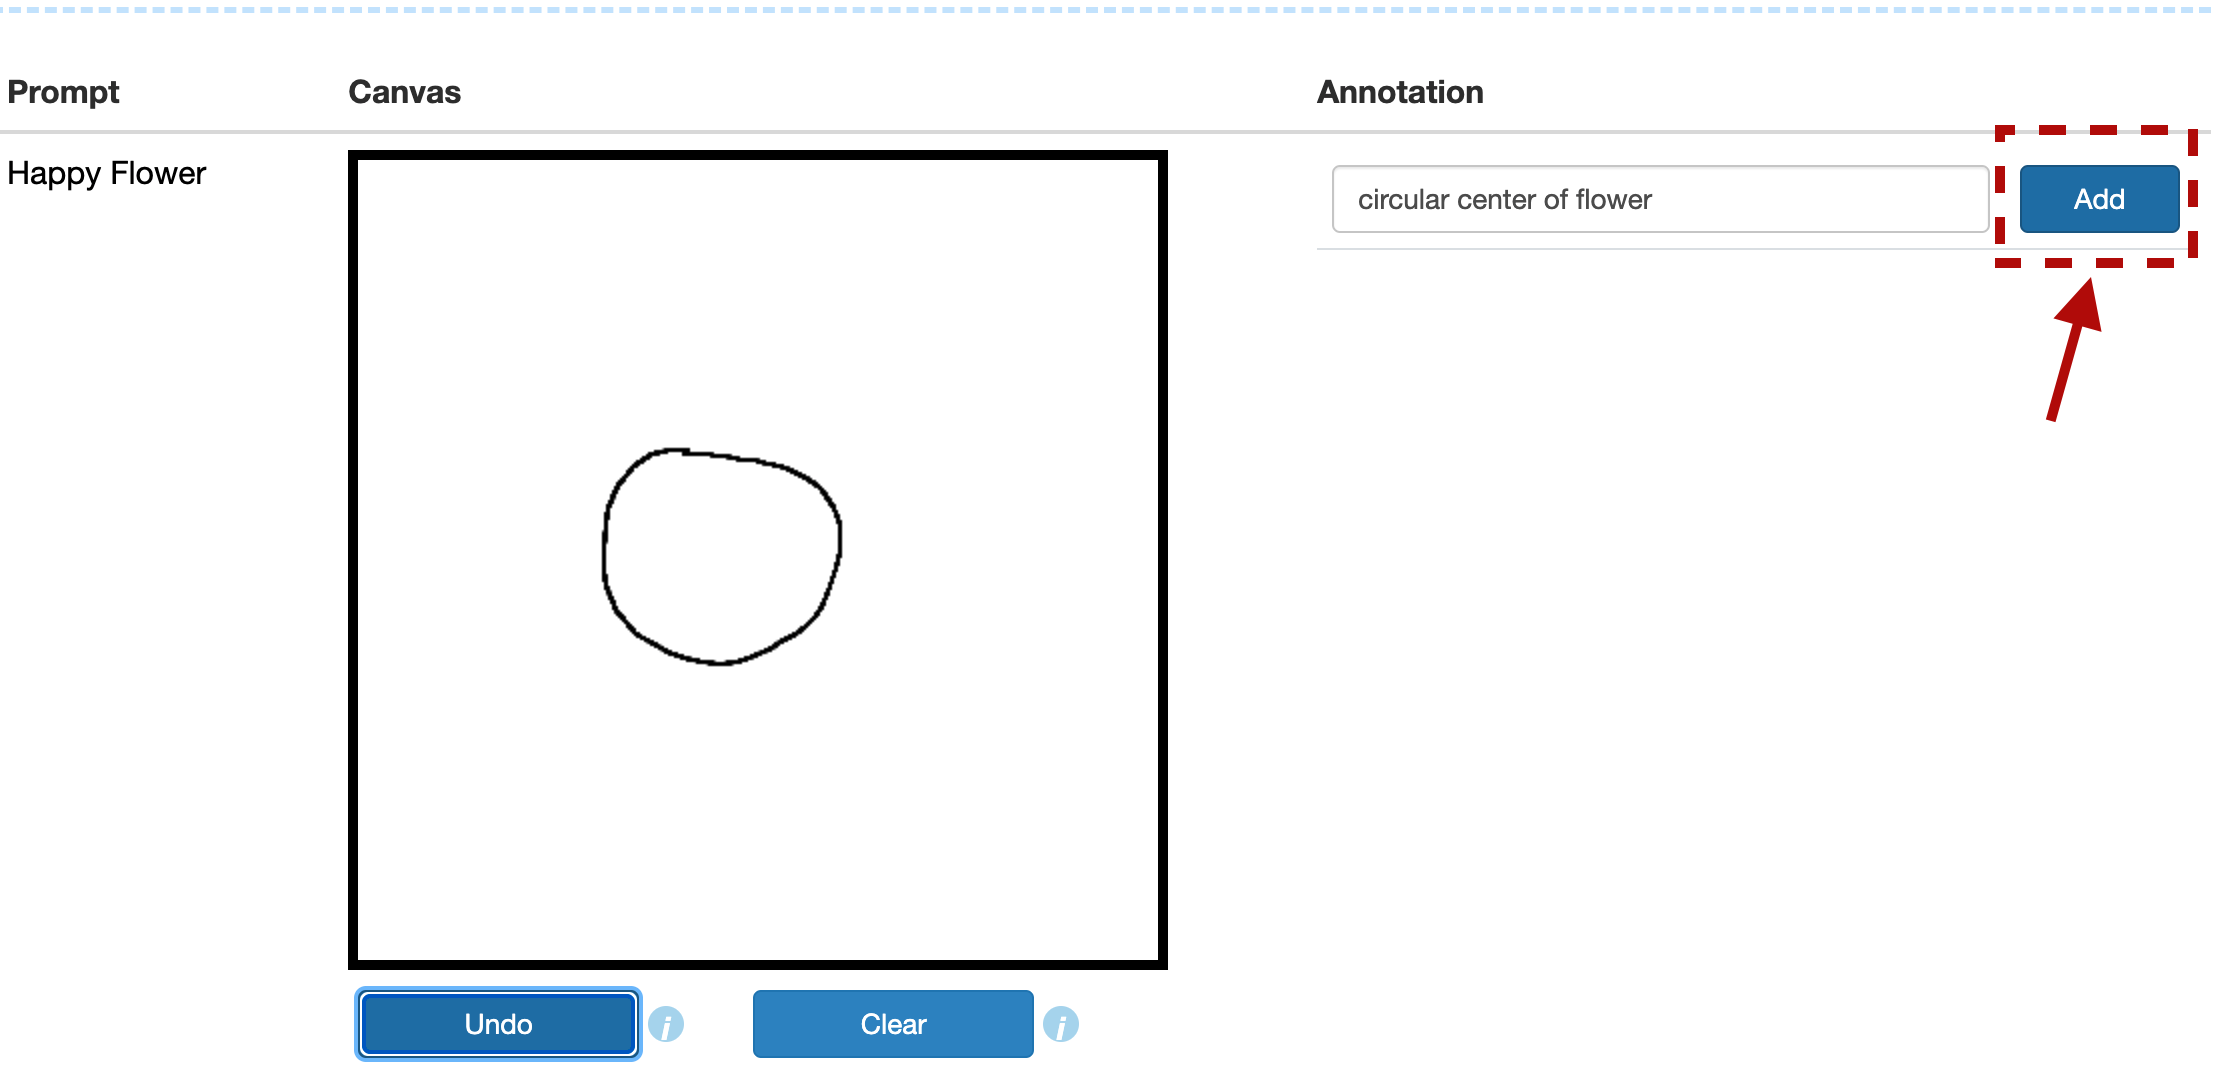
\includegraphics[width=.8\linewidth]{data_collection/v1_before_enter_text.png}  
    \caption{Main task interface before adding text descriptions for the drawing in the given step. Red arrow and box show where to click to add the text.}
    \label{v1.main_task.1.b}
\end{subfigure}
\end{figure*}

\begin{figure*}[!htb]
\ContinuedFloat
\begin{subfigure}{\textwidth}
    \centering
    % include third image
    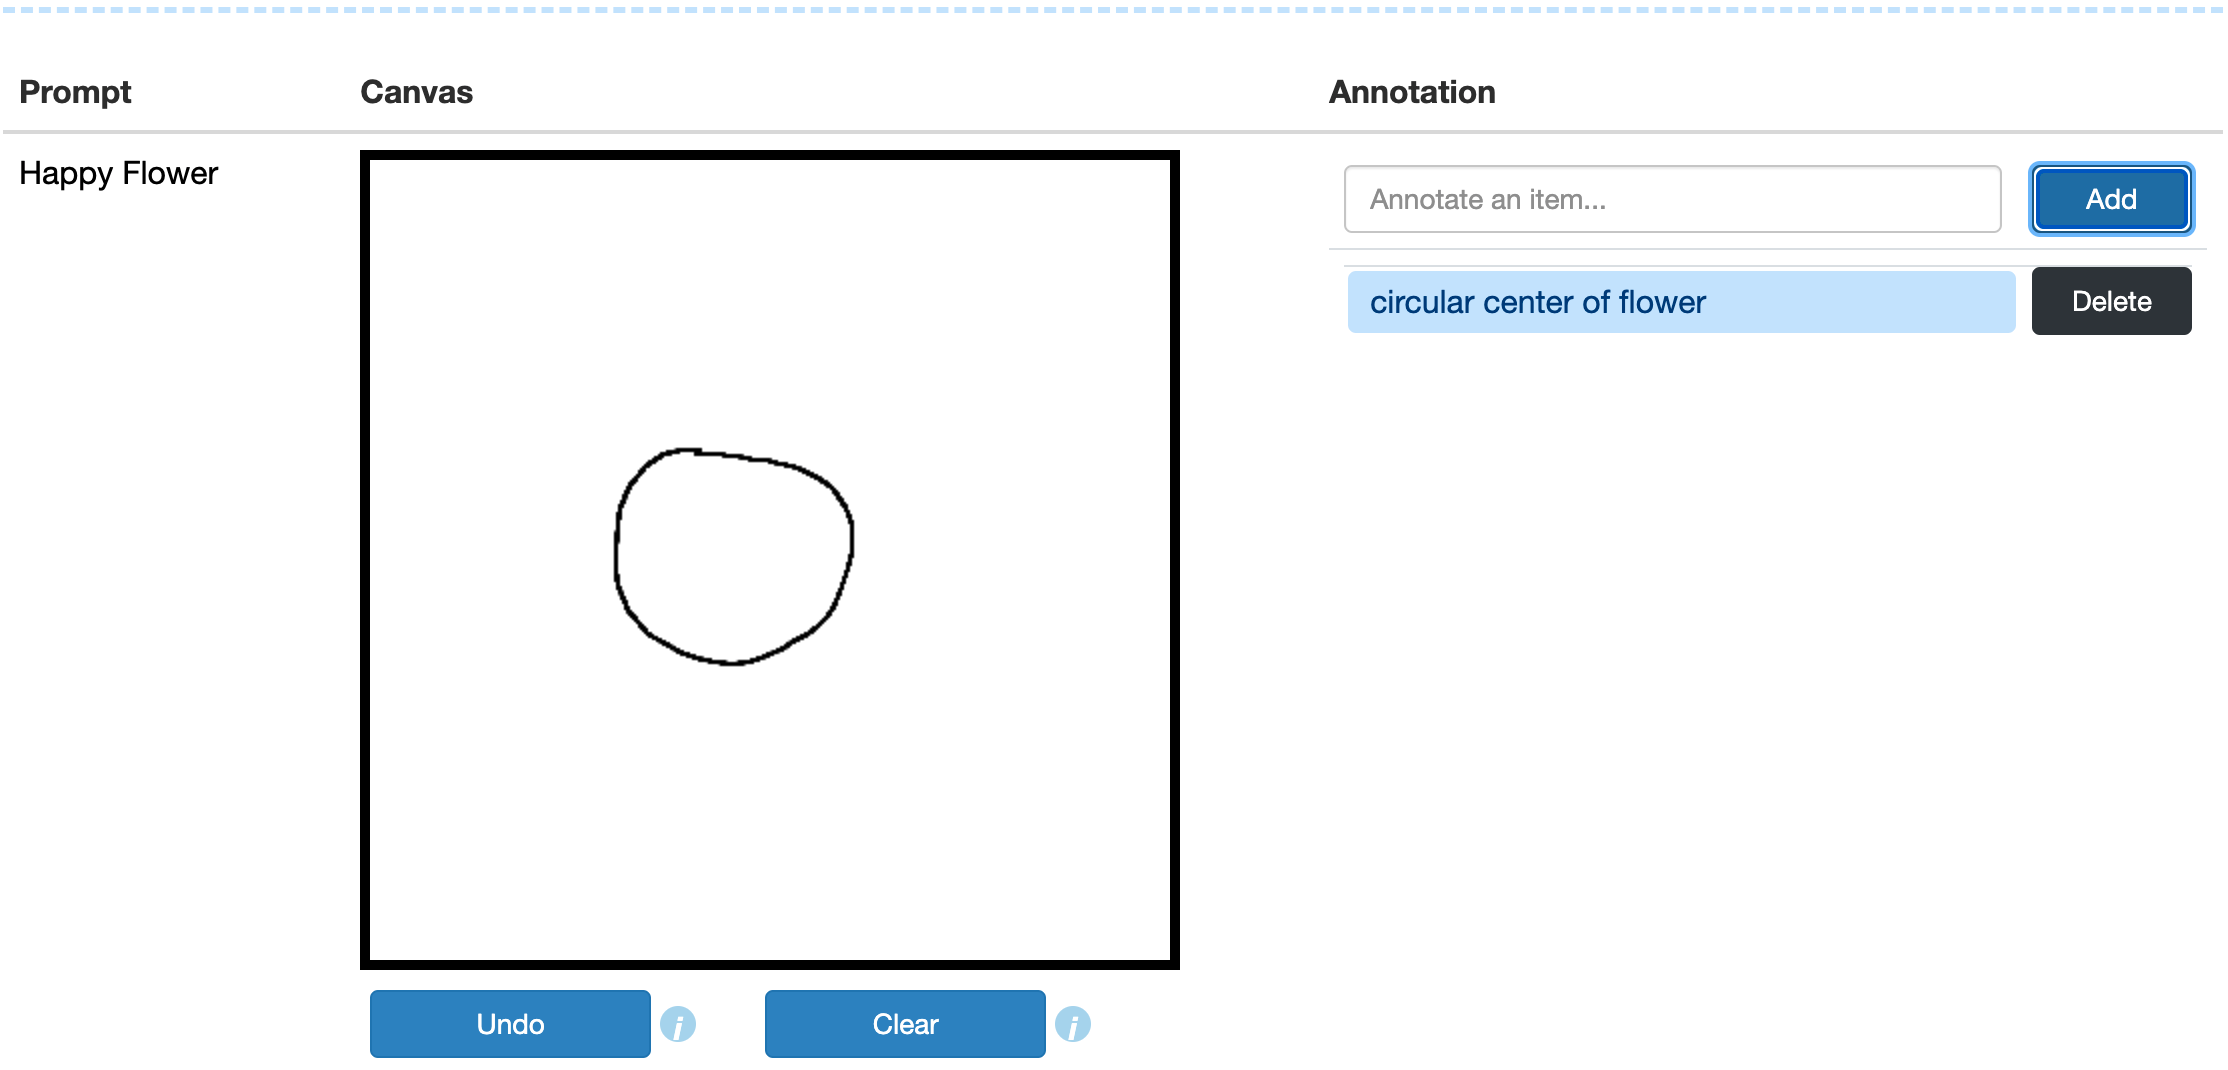
\includegraphics[width=.8\linewidth]{data_collection/v1_after_enter_text.png}  
    \caption{Main task interface after adding text descriptions for the drawing in the given step.}
    \label{v1.main_task.1.c}
\end{subfigure}
\caption{The ``drawing-and-adding'' functionality in Version 1. Repeat the above process for each step in a sketch.}
\label{v1.main_task.1}
\end{figure*}

We illustrate a typical annotation process with Version 1's interface in Figure \ref{v1.main_task.1}. 
The annotator starts with an empty canvas and empty table for textual descriptions, as shown in Figure \ref{v1.main_task.1.a}. For the annotator's convenience, we include a \textit{Undo} button and a \textit{Clear} button for erasing strokes and clearing the entire canvas.  
Then, the annotator draws a step in the sketch, and they would need to enter the text description for this step into the \textit{Annotation} column and hit \textit{Add} to display it as a new row in the annotation table. (Figure \ref{v1.main_task.1.b} and \ref{v1.main_task.1.c} show what the annotation table looks like before and after adding the texts for a given step.) If the annotator wants to remove an entire step, the objects in the drawing and the text description, they can use the \textit{Delete} button next to the texts to do so. An example is shown in Figure \ref{v1.main_task.delete}.
Repeat the drawing-and-adding process until the drawing is done. 
The design of a table for adding and deleting text annotations intends to encourage turkers to break their drawing into a series of semantically meaningful parts, responding to principal \ref{data_design_2} and \ref{data_design_3}.  Enabling users to be able to delete each component is also demonstrative of these two principals. 


\begin{figure*}[!htb]
\begin{subfigure}{\textwidth}
    \centering
    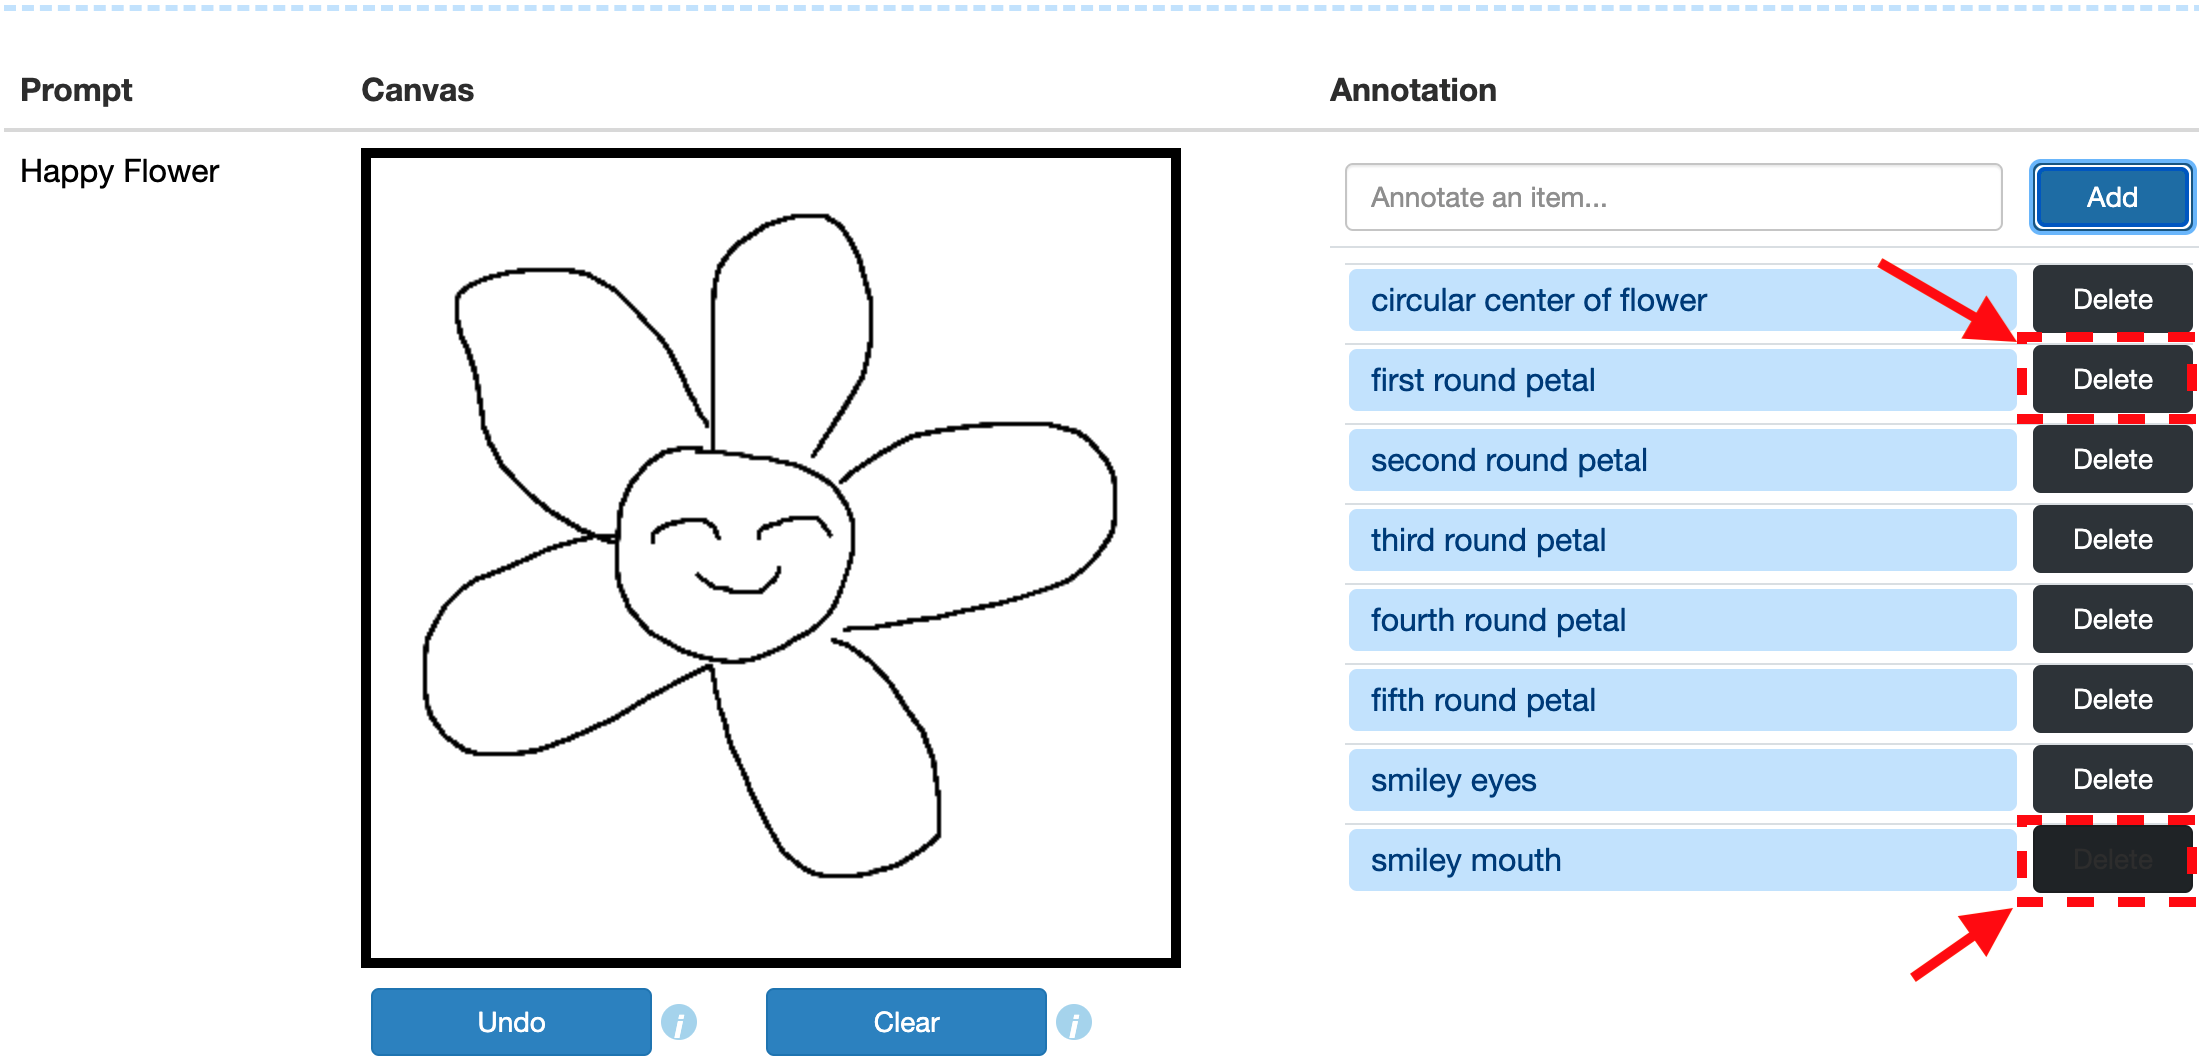
\includegraphics[width=.8\linewidth]{data_collection/v1_before_delete.png}  
    \caption{A complete annotation for the prompt \textit{Happy Flower}. Red arrows and boxes point to \textit{Delete} buttons that can be used to delete the steps associated with the textual annotaitons, if the annotator is not satisfied with the steps.}
    \label{v1.main_task.delete.a}
\end{subfigure}
\newline
\begin{subfigure}{\textwidth}
    \centering
    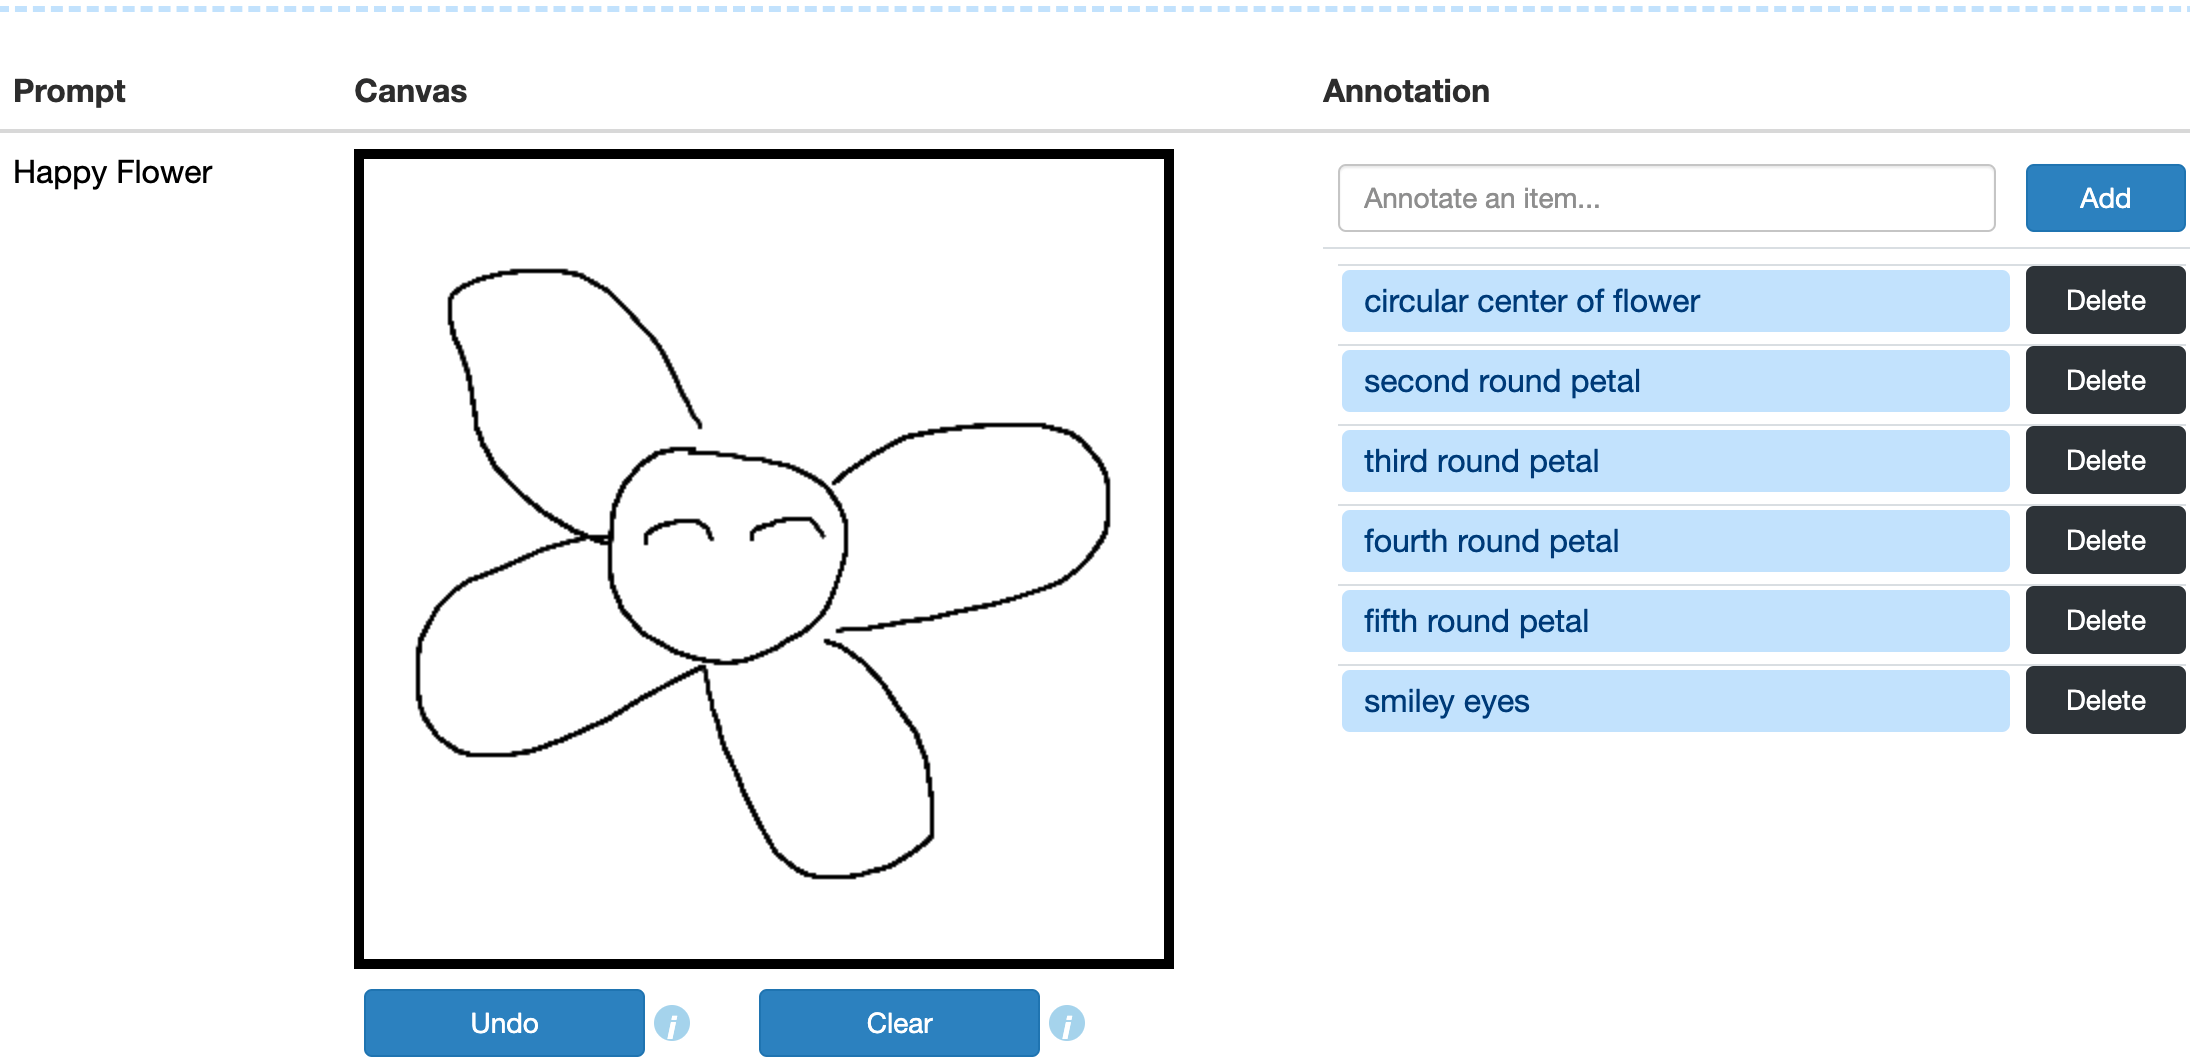
\includegraphics[width=.8\linewidth]{data_collection/v1_after_delete.png}  
    \caption{Main task interface after the two steps associated with \textit{first round petal} and \textit{smiley mouth}, respectively.}
    \label{v1.main_task.delete.b}
\end{subfigure}
\caption{Demonstrating the functionality of the \textit{Delete} button.}
\label{v1.main_task.delete}
\end{figure*}

We encountered some difficulties when implementing the \textit{Delete} functionality. At the beginning, we treated erasing strokes as drawing the same strokes but in white color; however, when strokes overlap each other, overwriting with white strokes would break other strokes into segments. Therefore, we designed the drawing canvas to use layers like Photoshop, so that deleting strokes would be the same as deleting an entire layer, thus leaving other strokes intact.   

\subsubsection{Instruction and Requirement}

\begin{figure*}[!htb]    
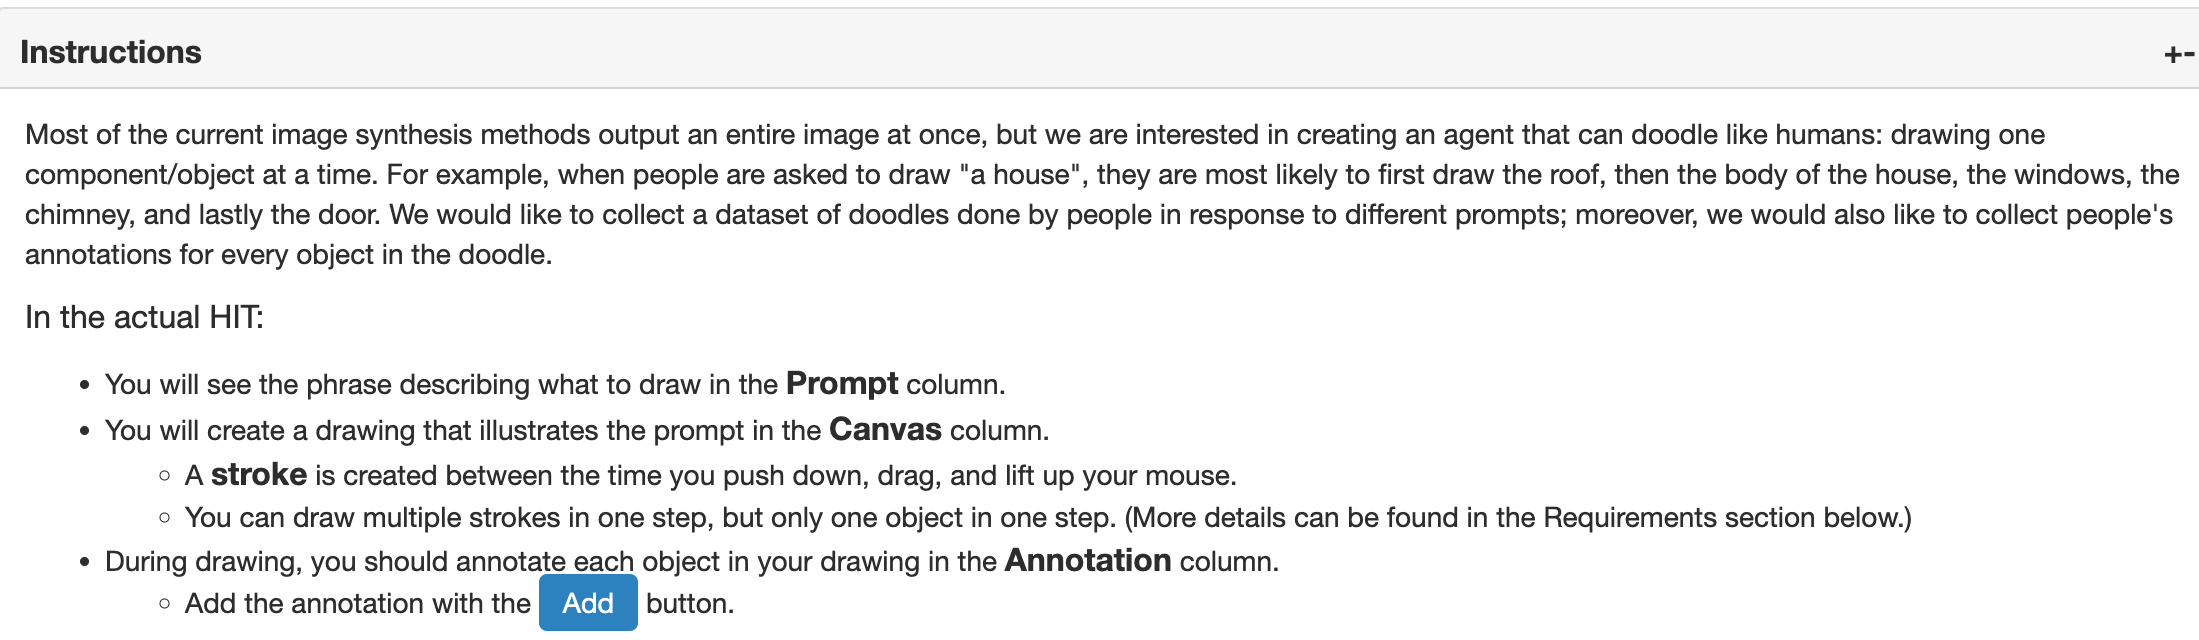
\includegraphics[width=\linewidth]{data_collection/v1_instruction.png} 
\caption{Instruction section of Version 1.}
\label{v1.instruction}
\end{figure*}

We show the layout of the instructions in Figure \ref{v1.instruction}. We begin the instruction by giving a short explantion on the motivation behind collecting this dataset to prime turkers for good-quality annotations, since they would understand more about what the purpose for collecting this dataset. What we struggled the most when drafting the requirements was deciding what would be a single \textit{step} in drawing and how do we clearly explain this definition to the turkers? In Version 0, we relied on common geometric shapes to decompose a drawing into a sequence of steps. In Version 1, we considered asking turkers to annotate for each stroke in the drawing, but we quickly ruled out this option since it was time-consuming, and it did not align with how the instructor taught the child in the \textit{How To Draw a Cute Ice-Cream Cone} video. We decided that turkers should annotate for each \textit{object} in the drawing. The ambiguity around the word \textit{object} has posed the biggest challenge in defining a clear set of requirements. For example, when drawing for the prompt \textit{Happy Face}, one reasonable decomposition is annotating for 4 steps: face, eyes, mouth, and the face contour. However, for someone who draws very detailed eyes, they might want to annotate for the shape of the eye socket and the length of the eye lashes. So what level of specificity should be allowed?  
There is a wide spectrum of allowed annotations depending on how a person approaches drawing for the give prompt. Indeed, the great variation and uncertainty that comes from individuality and personal styles demonstrated through drawings would eventually drive us to not collect drawings and simply ask for text annotations for sketches found in existing datasets.  
At the time, we resorted to repeatedly testing the interface with lab mates to refine the requirements. Here is an excerpt from an old version of the instructions, in which we tried to explain a single \textit{step} of the annotation:
\begin{quotation}
In each task, we show \textbf{1 prompt} from which we would like to get
\begin{enumerate}
    \item A drawing containing 1 \textbf{entity} that you think illustrates the prompt.
    \item Text annotation for every \textbf{``component''} that makes up the entity.
    The word ``component'' is intentially vague, and it depends on how you compose your drawing. For example, in the above example, the prompt is ``smiley face'', and during the process of creating a ``smiley face'' entity, we used 4 components: a face, a left eye, a right eye, and a mouth. For each component, you can annotate with ``face'', ``left eye'', ``right eye'', ``mouth'', respectively; you can also annotate with more details describing the shapes of each component: ``face that looks like an arc opening downwards'', ``a left eye that is an arc'', ``a right eye that looks exactly like the left eye'', ``an arc-like mouth''. Try to use creative and descriptive languages. You can draw a component using multiple strokes.
\end{enumerate}
\end{quotation}
We also need to come up with examples explaining each requirement. We select a few major sub-versions of the requirements resulted from circulating the interface within our lab.  

Requirements and selected examples used in the first release in lab (Item 1 to 3 meant to enforce principal \ref{data_design_1}; Item 4 to 6 for \ref{data_design_2} and \ref{data_design_3}):
\begin{enumerate}
\item Do not draw entity that does not respond to the prompt. For example, given the prompt \textit{Smiley Face}, the drawing should not contain irrelevant objects like a house. 
\item Do not draw more than one entity that responds to the prompt. For example, One should not draw two \textit{Smiley Face} entities, although each \textit{Smiley Face} entity is good. However, you can draw multiple tree objects to illustarte the prompt \textit{Forest}.  
\item \label{v1_requirement1_3} Do not draw entity that is ambiguous in terms of illustrating the prompt. For example, the drawing (Figure \ref{v1.requirement_1.1}) looks more like a \textit{Sad Face} than \textit{Smiley Face}.
\item Do not draw one component that contains more information/content than what the annotation for that component describes. (A counterexample is illustrated in Figure \ref{v1.requirement_1.2}.)
\item Do not split the drawing of a component into multiple steps, unless you can annotate each step separately. (A counterexample is illustrated in Figure \ref{v1.requirement_1.3}.)
\item Do not annotate a component more than once.
\end{enumerate}

\begin{figure*}[!htb]
\begin{subfigure}{0.5\textwidth}
    \centering
    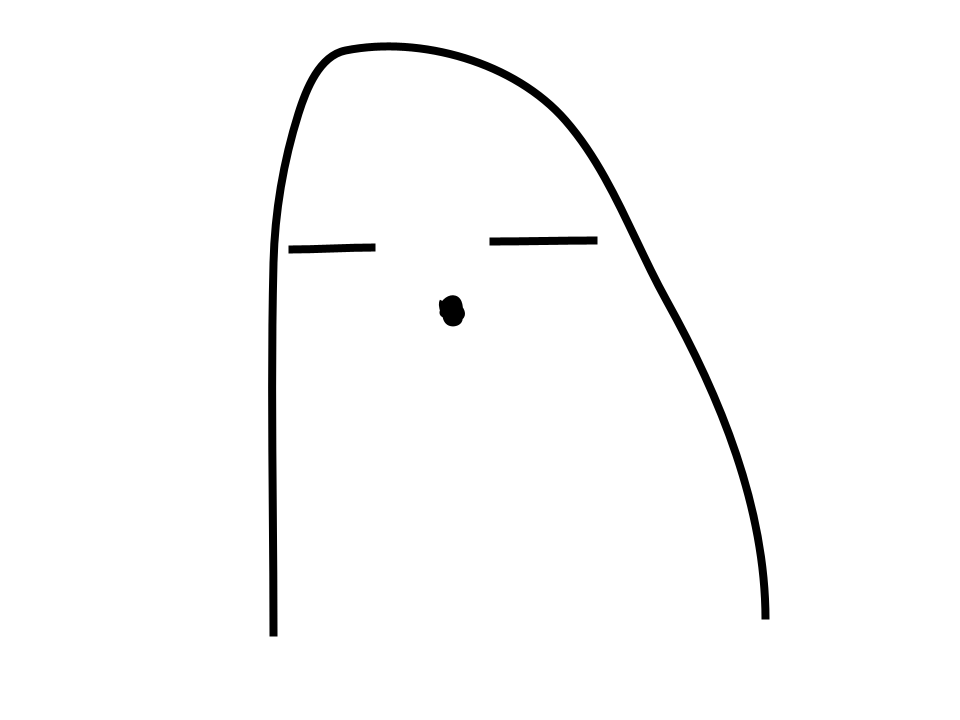
\includegraphics[width=.4\linewidth]{data_collection/host_amazon/hit_1/bad_smiley_face_ambiguous_face.png}  
    \caption{An example included in the first version of the requirements, explained in more details in item \ref{v1_requirement1_3}.}
    \label{v1.requirement_1.1}
\end{subfigure}
\end{figure*}

\begin{figure*}[!htb]
\ContinuedFloat
\begin{subfigure}{\textwidth}
    \centering
    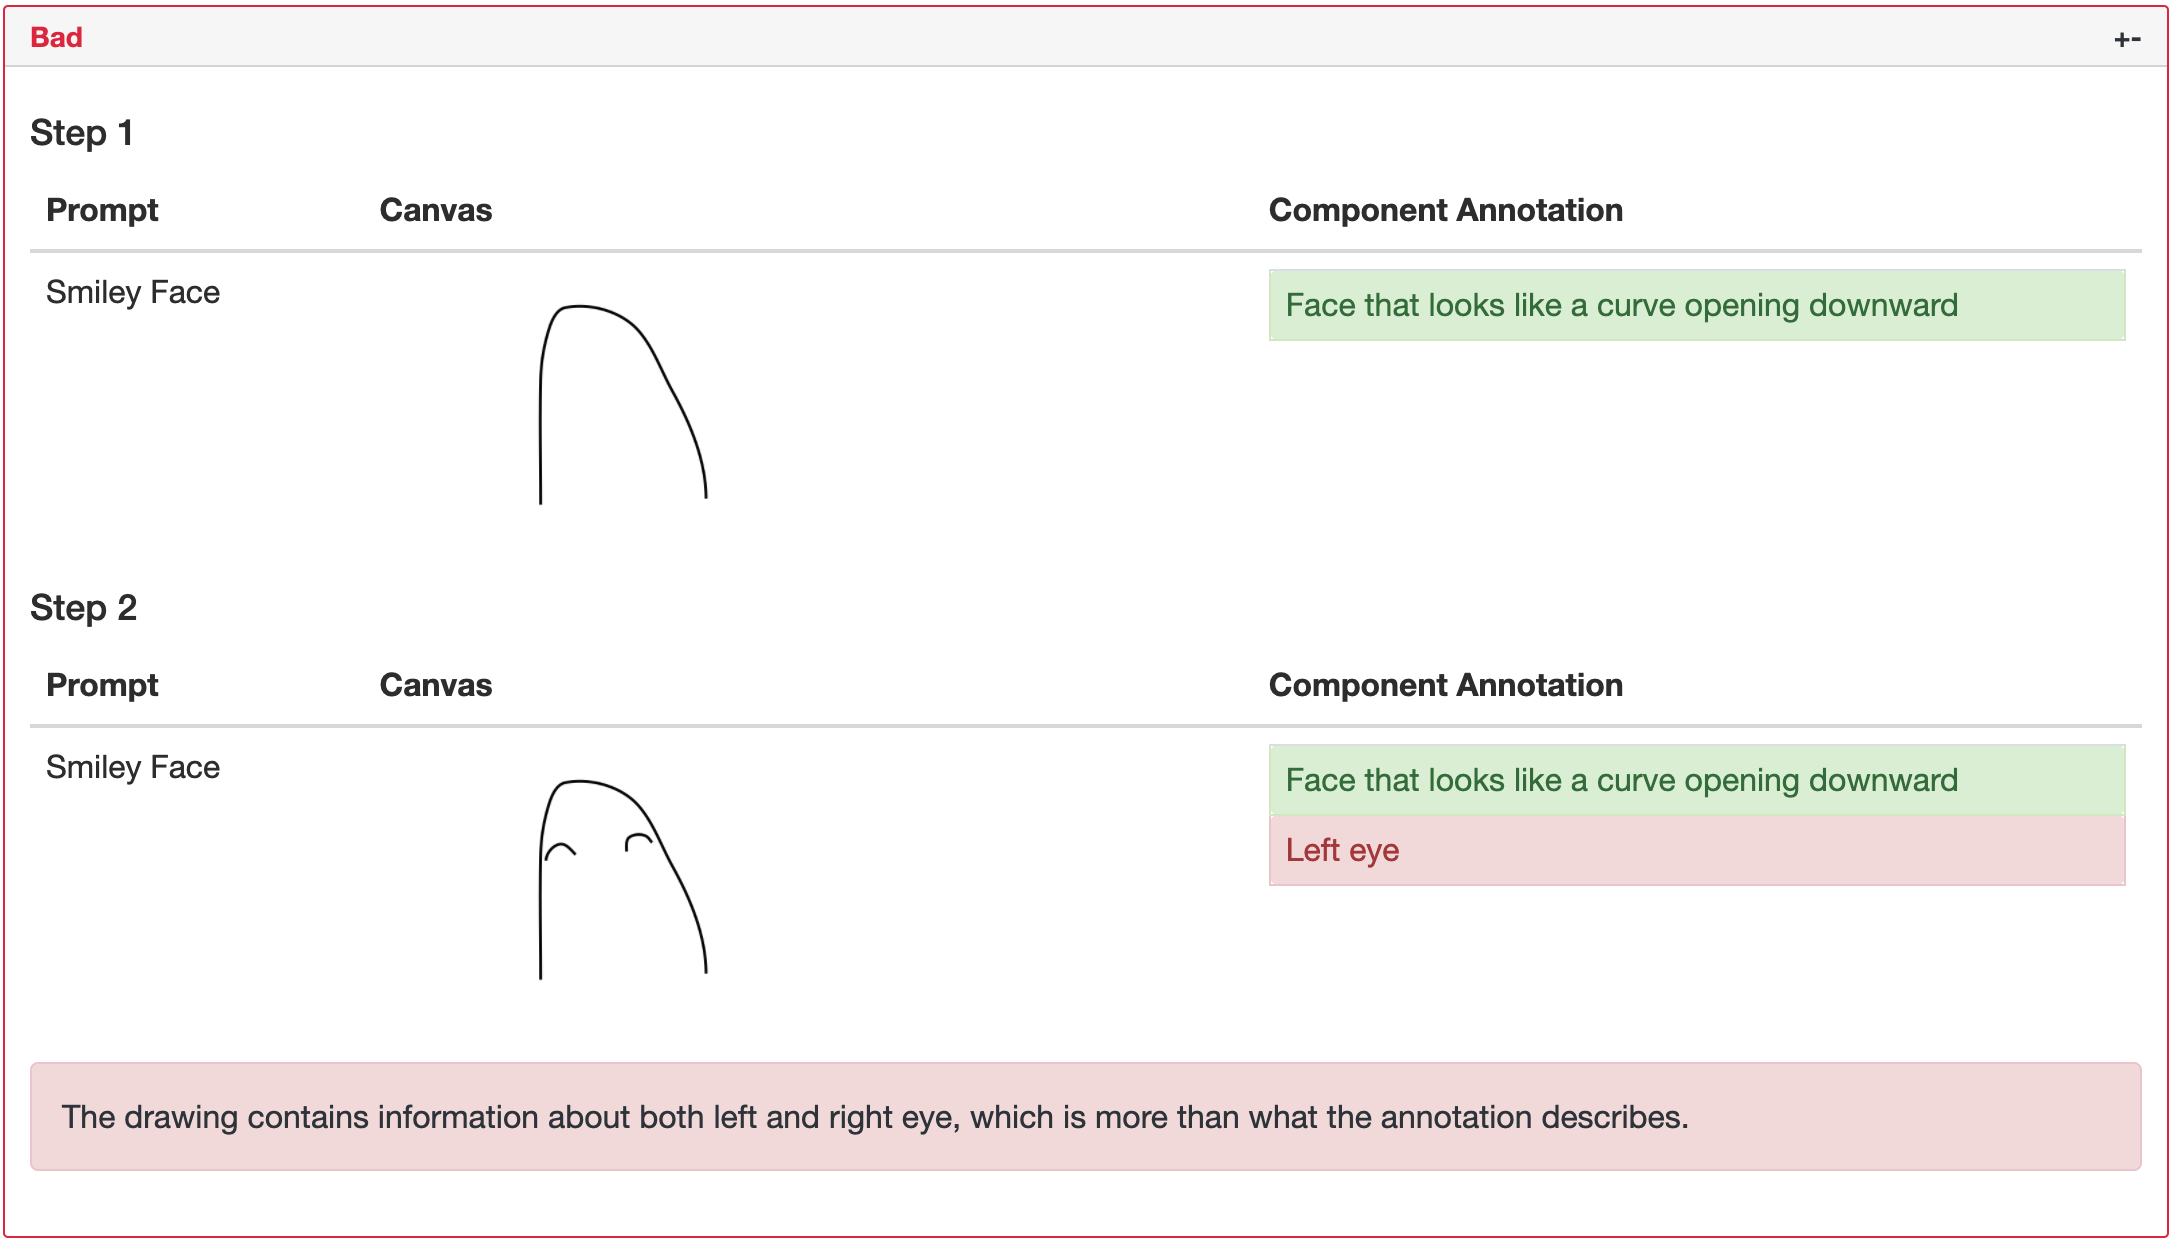
\includegraphics[width=.8\linewidth]{data_collection/v1_requirement1_bad1.png}  
    \caption{Unaligned drawing and text description.}
    \label{v1.requirement_1.2}
\end{subfigure}
\newline
\begin{subfigure}{\textwidth}
    \centering
    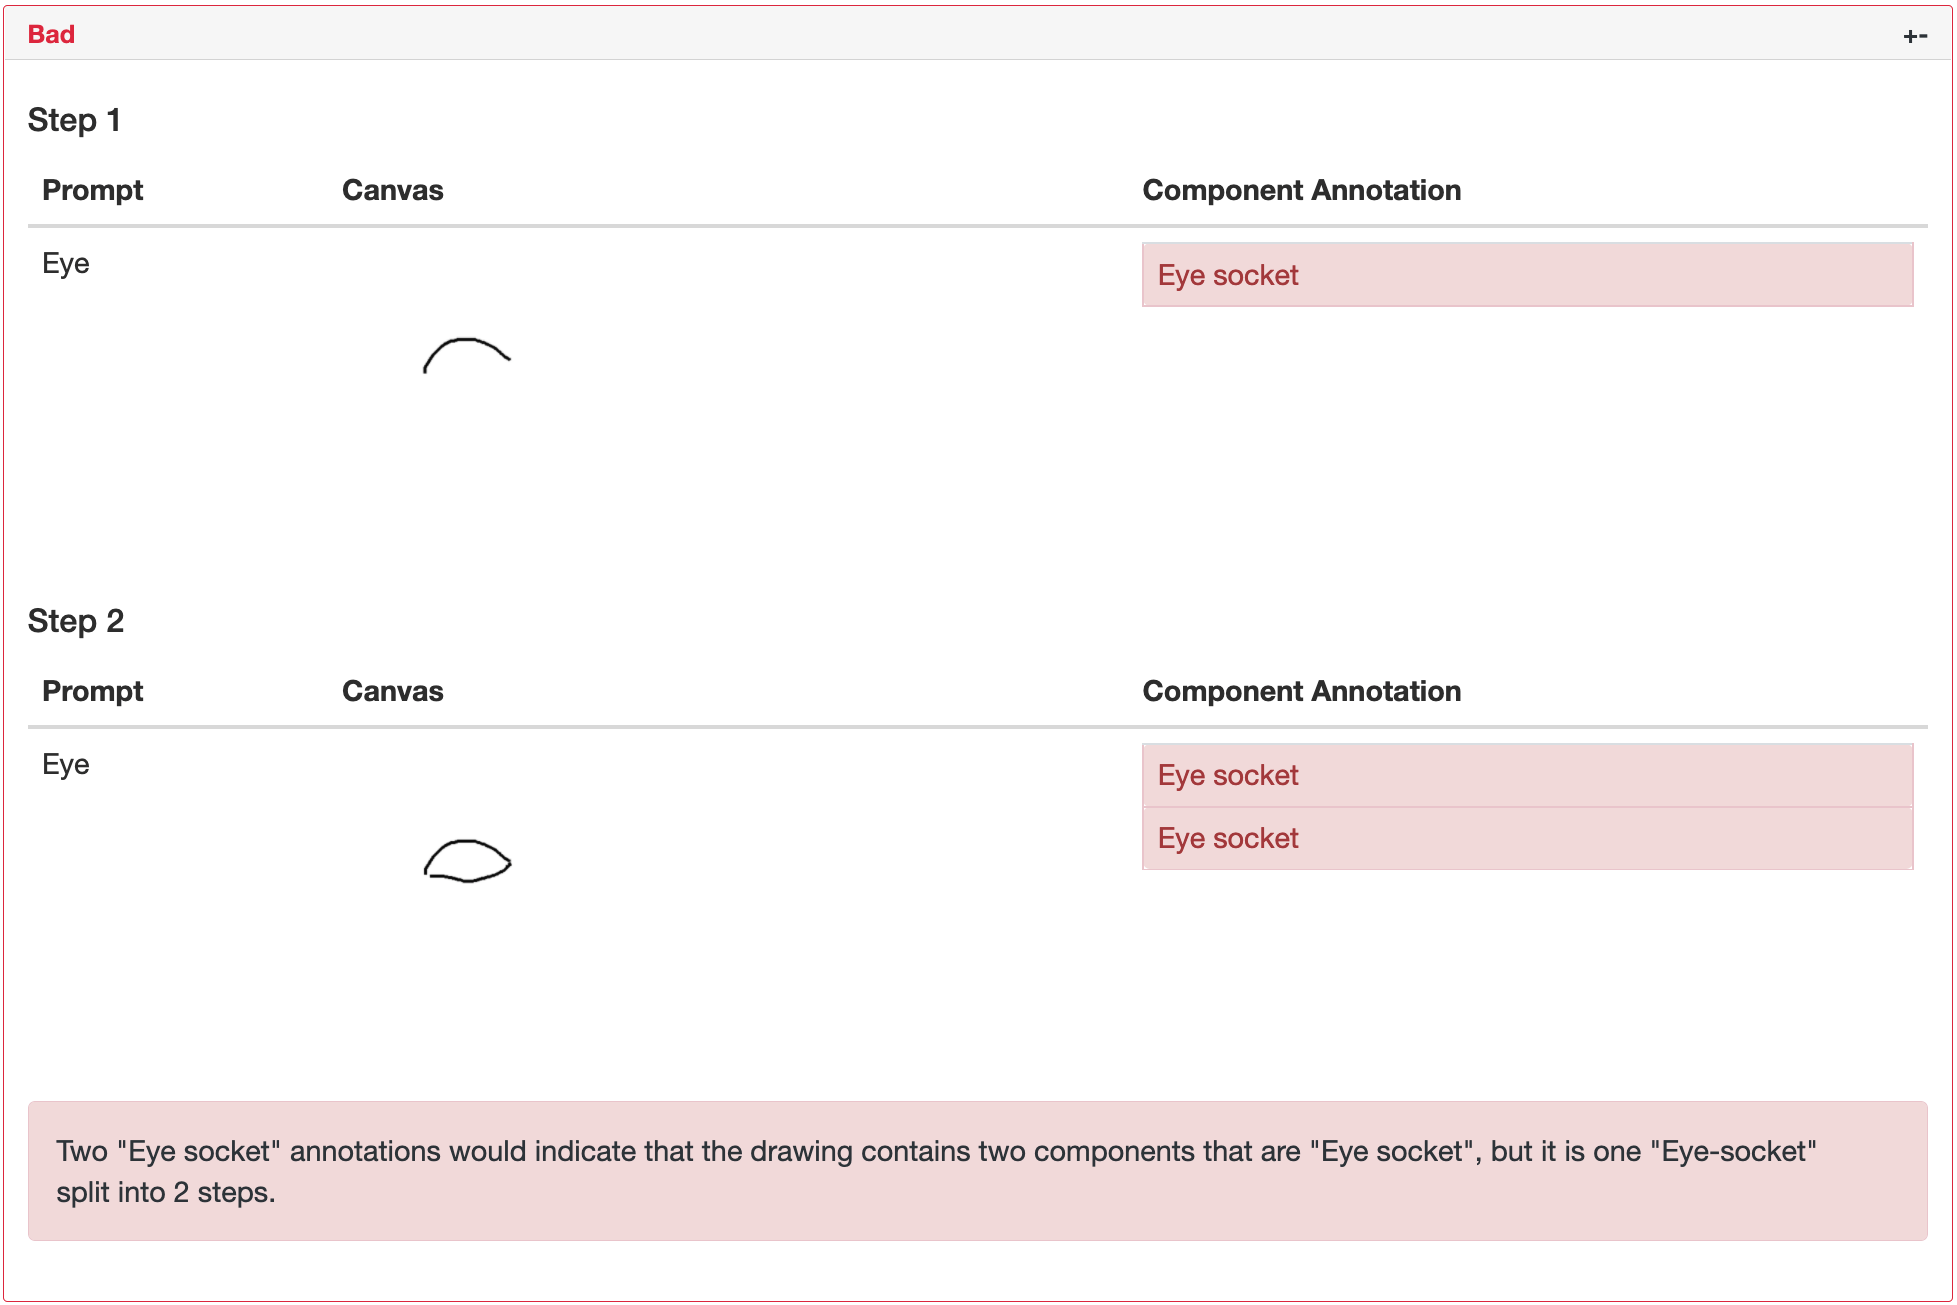
\includegraphics[width=.8\linewidth]{data_collection/v1_requirement1_bad2.png}  
    \caption{An example of misalignment: text description \textit{overflow} into multiple steps.}
    \label{v1.requirement_1.3}
\end{subfigure}
\caption{Screenshots of counterexamples used in first version of the requirements in Version 1.}
\label{v1.requirement_1}
\end{figure*}
% Figure 3x.a and 3x.b show some previous versions of the requirements. We eventually decided that  

% There is even more effort that went into defining the requirements of the task. This is really the section that we want to use to enforce all the DQ's. The final set of instructions is displayed in Figure x4.
% [Figure x4: final requirements]

% Comparing examples in requirements format:

% Methods to help understand the requirements. 
% Specifying which examples demonstrate which requirements, add next to the questions which requirement the question is testing. 

Requirements and selected examples used in the second release in lab (Item 4 is meant to enforce principal \ref{data_design_1}; the other items for \ref{data_design_2} and \ref{data_design_3}):
\begin{enumerate}
\item Draw \textit{one} item at a time and provide its corresponding annotation. For example, the text annotation says ``left eye'', but two items are drawn: a left eye and a right eye.
\item The annotation should describe its corresponding item in the drawing \textit{entirely}.
\item The annotation should name the item.
\item Desired properties of good drawings:
\begin{itemize}
    \item Contain as many items as possible, but be sure that they all contribute to illustrating the prompt. For example, draw more than just two eyes for a face.
    \item Use shapes creatively. For example, draw a triangle for the left eye, and annotate accordingly with ``triangular left eye that shows suspicion''.
\end{itemize}
\item Desired properties of good annotations:
\begin{itemize}
    \item Use descriptive languages. For example, ``a left eye that looks an arc facing downward''.
    \item Include the intention/purpose of drawing an item. Explain in the annotation reasons for drawing the item. For example, ``thumbs-up next to the face that really shows how happy the face is''.
\end{itemize}
\end{enumerate}

Requirements and selected examples used in the third release in lab (Item 1 is meant to enforce principal \ref{data_design_1}; the other items for \ref{data_design_2} and \ref{data_design_3}):
\begin{enumerate}
\item Each drawing should contain at least 2 steps.
\item Annotation of each step should include at least the name of the drawn object(s).
\item If draw multiple copies of the same object, draw each object in a separate step and give different annotations by using, for example, cardinal or ordinal numbers. (An example shown in Figure \ref{v1.requirement_3})
\item Differentiate between plural and singular forms.
\item The name of the whole should not be used for its parts. (An example shown in Figure \ref{v1.requirement_3})
\item The word "right" always refers to this side: $\Longrightarrow$
\end{enumerate}

\begin{figure*}[!htb]
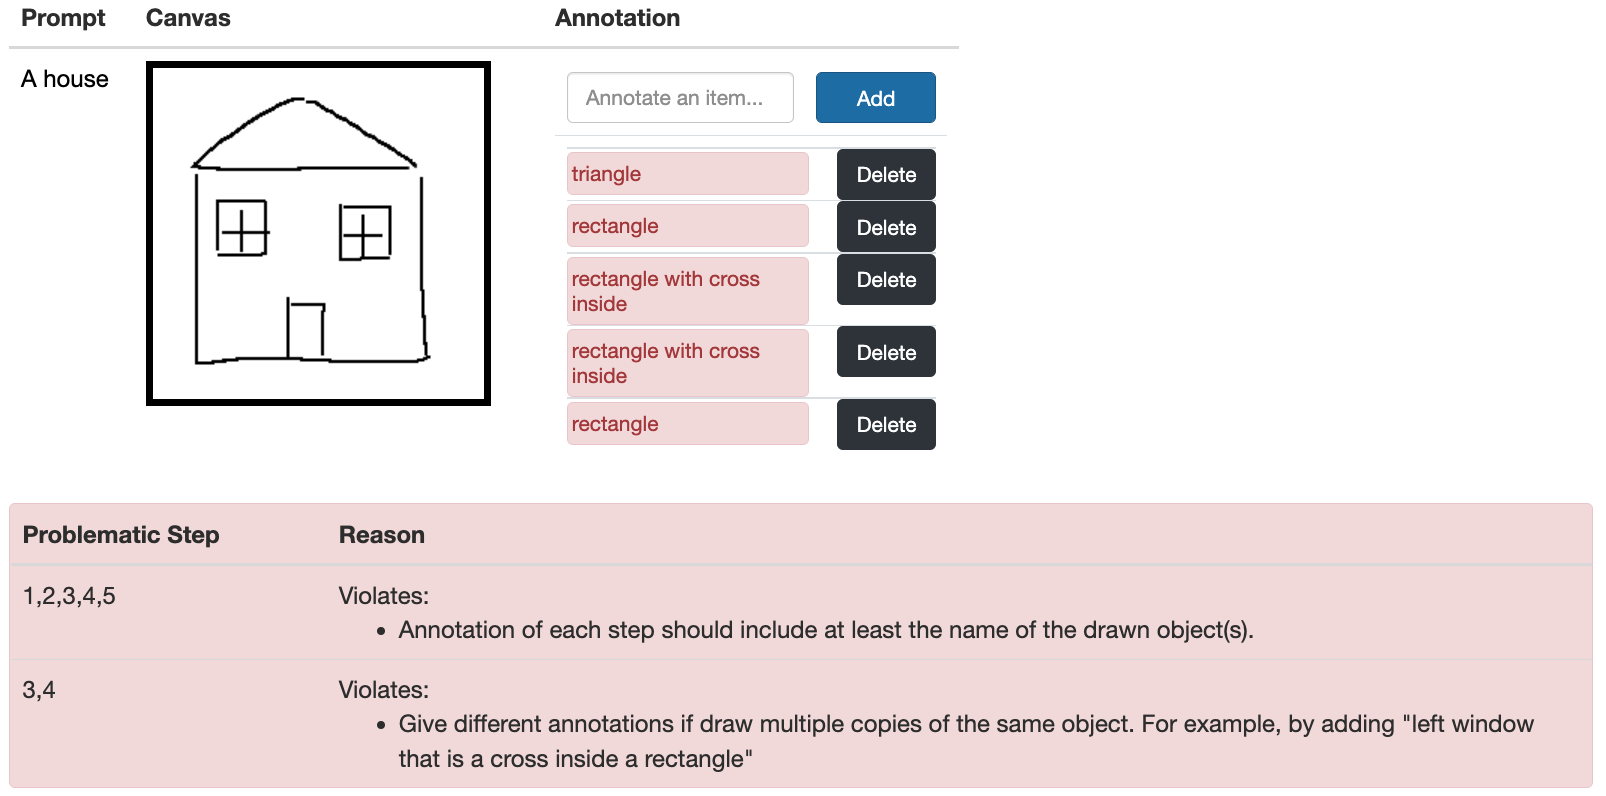
\includegraphics[width=.8\linewidth]{data_collection/v1_requirement3_bad1.png}  
\caption{Screenshots of counterexamples used in third version of the requirements in Version 1.}
\label{v1.requirement_3}
\end{figure*}

After a series of smaller changes, we eventually arived at the final version of the requirements for Version 1, as shown in Figure \ref{v1.requirement}. Most of the requirements are dedicated to ensure principle \ref{data_design_2} and \ref{data_design_3}. Requirement 1 ensures that no irrelevant sketches and trivial annotations are provided, and we resort to good faith that the annotators would provide a sketch that illustrates the given prompt. As expected, problems related to ambiguous sketches and unaligned text annotations surfaced after the deployment on AMT, eventually resulting in a complete change in format and lead to Version 2.     

\begin{figure*}[!htb]
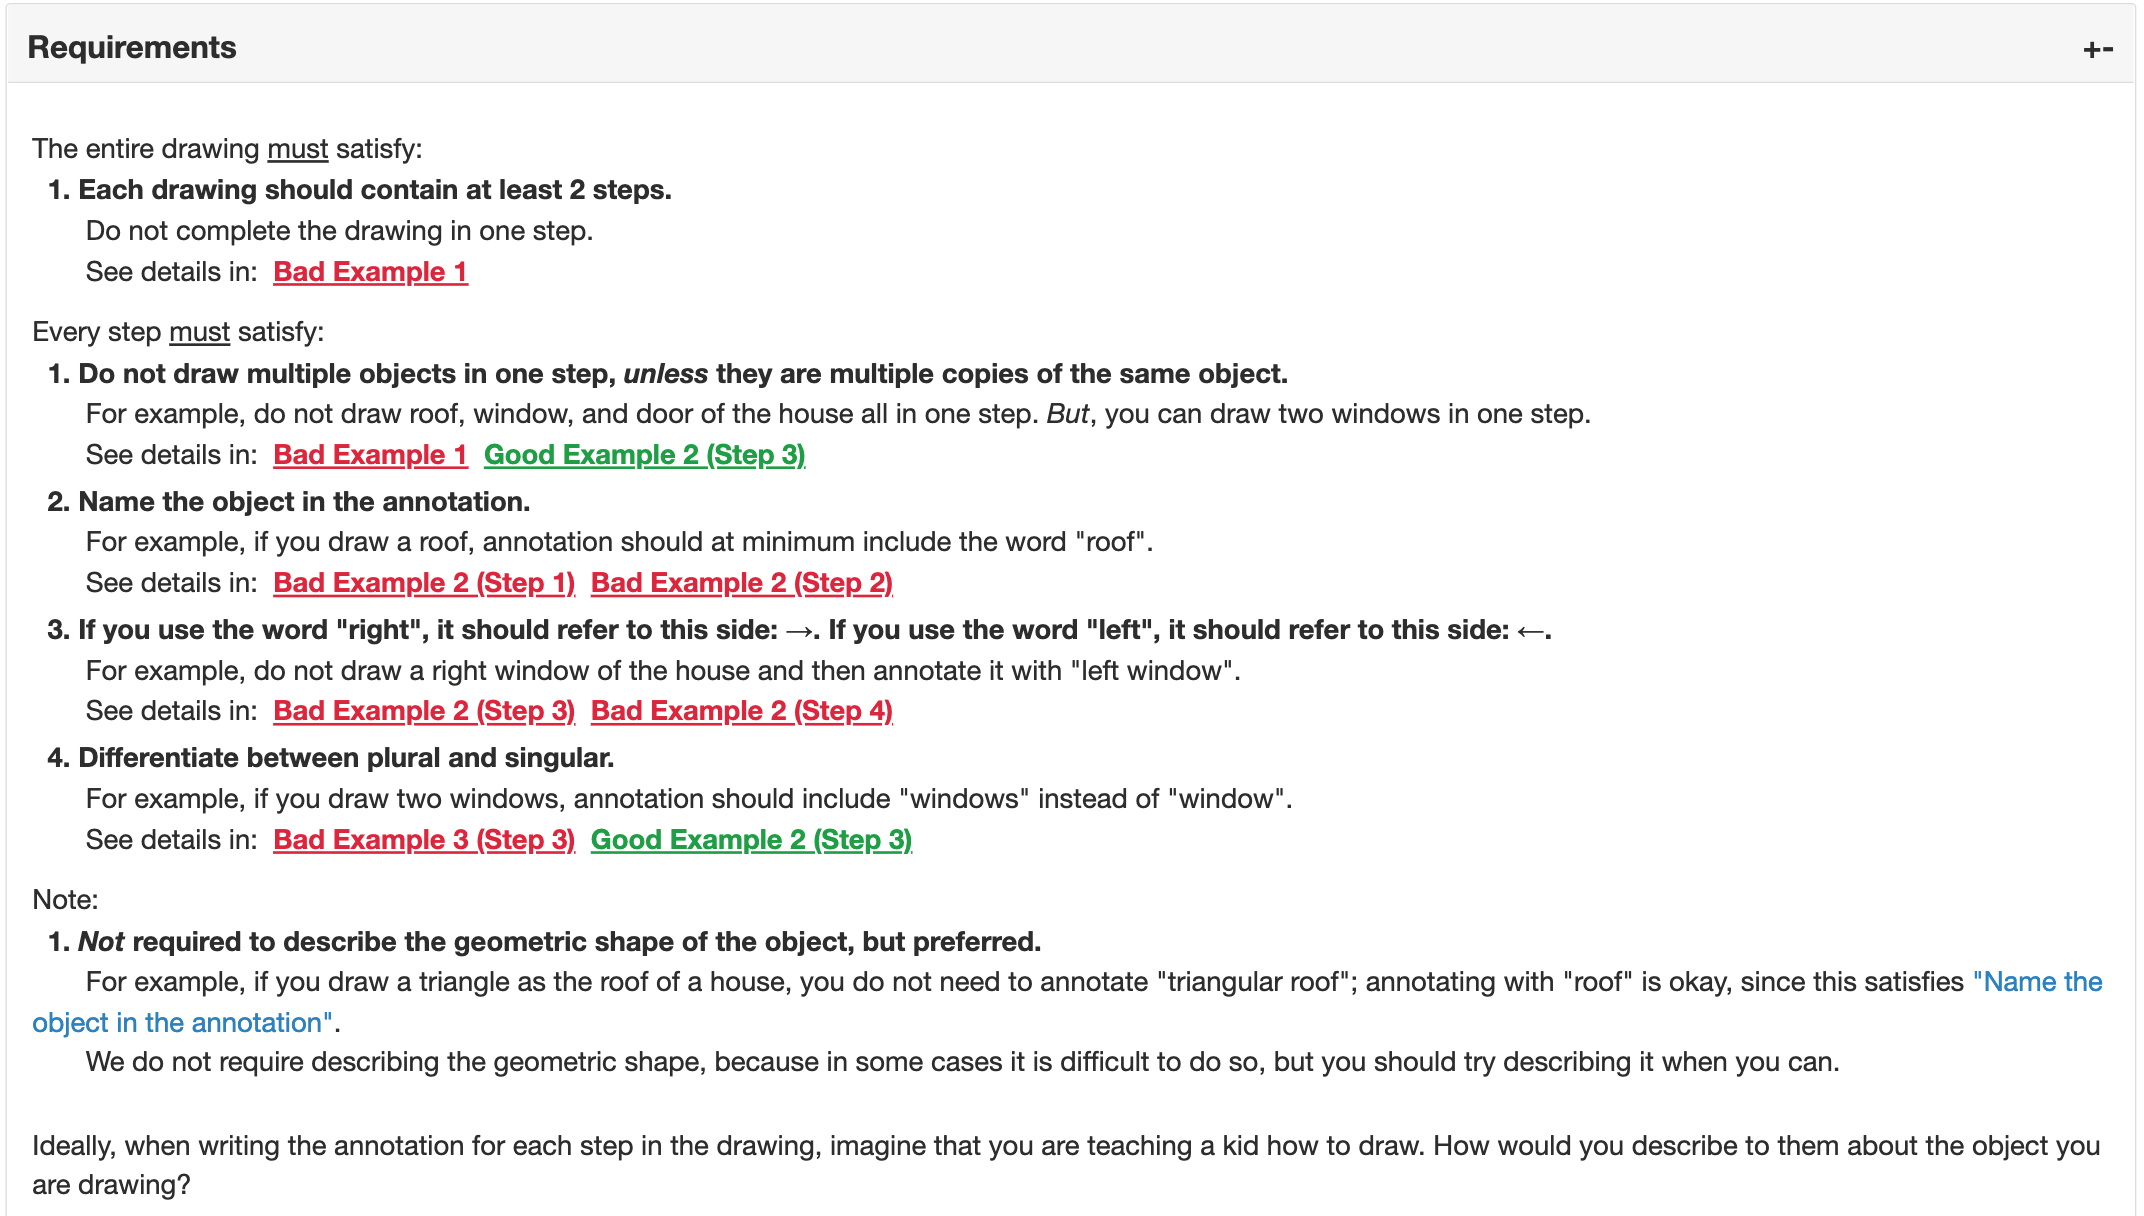
\includegraphics[width=\linewidth]{data_collection/v1_requirement.png}  
\caption{Screenshots of final version of the requirements in Version 1. The \textcolor{red}{\underline{Bad Example}} links to counter-examples of the requirements, and \textcolor{green}{\underline{Good Example}} links to good examples. When turkers click on the links, they are directed to the examples illustrating the corresponding requirement.}
\label{v1.requirement}
\end{figure*}

\begin{figure*}[!htb]
\begin{subfigure}{\textwidth}
\centering
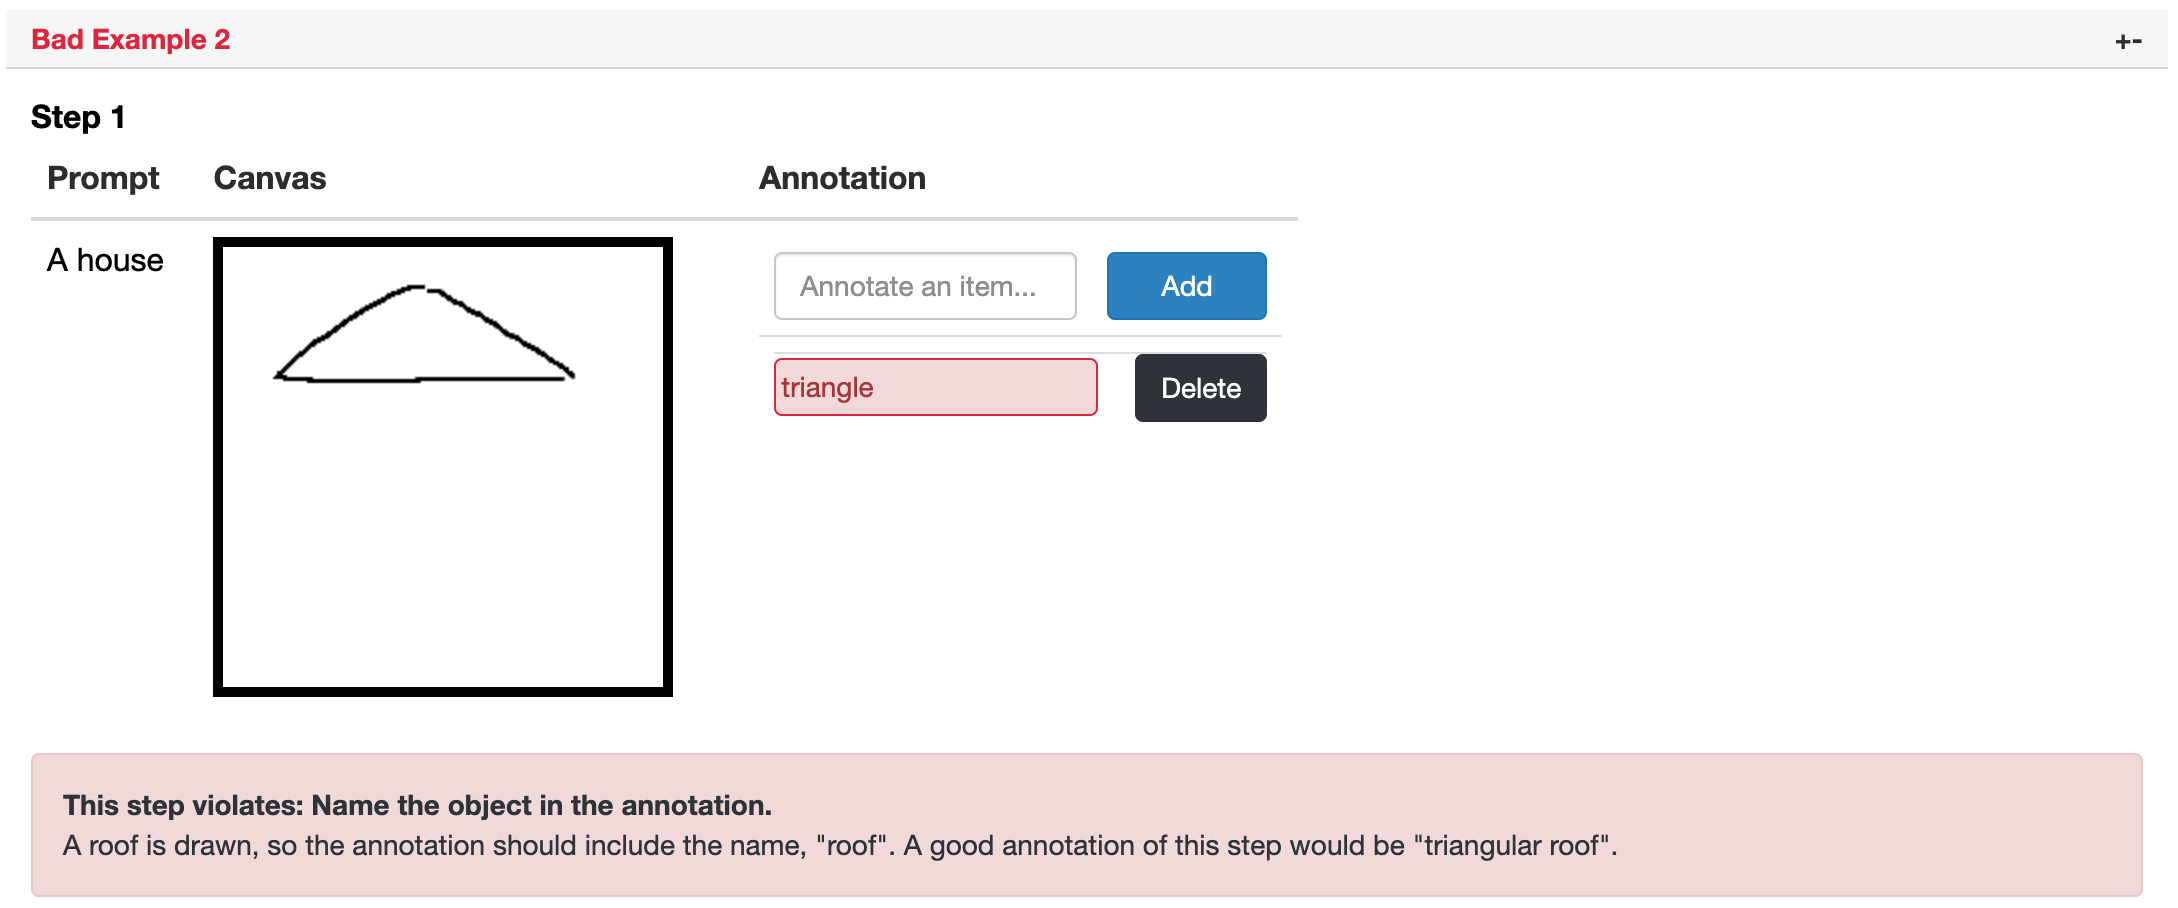
\includegraphics[width=.8\linewidth]{data_collection/v1_badeg_1.png}  
\end{subfigure}
\newline
\begin{subfigure}{\textwidth}
\centering
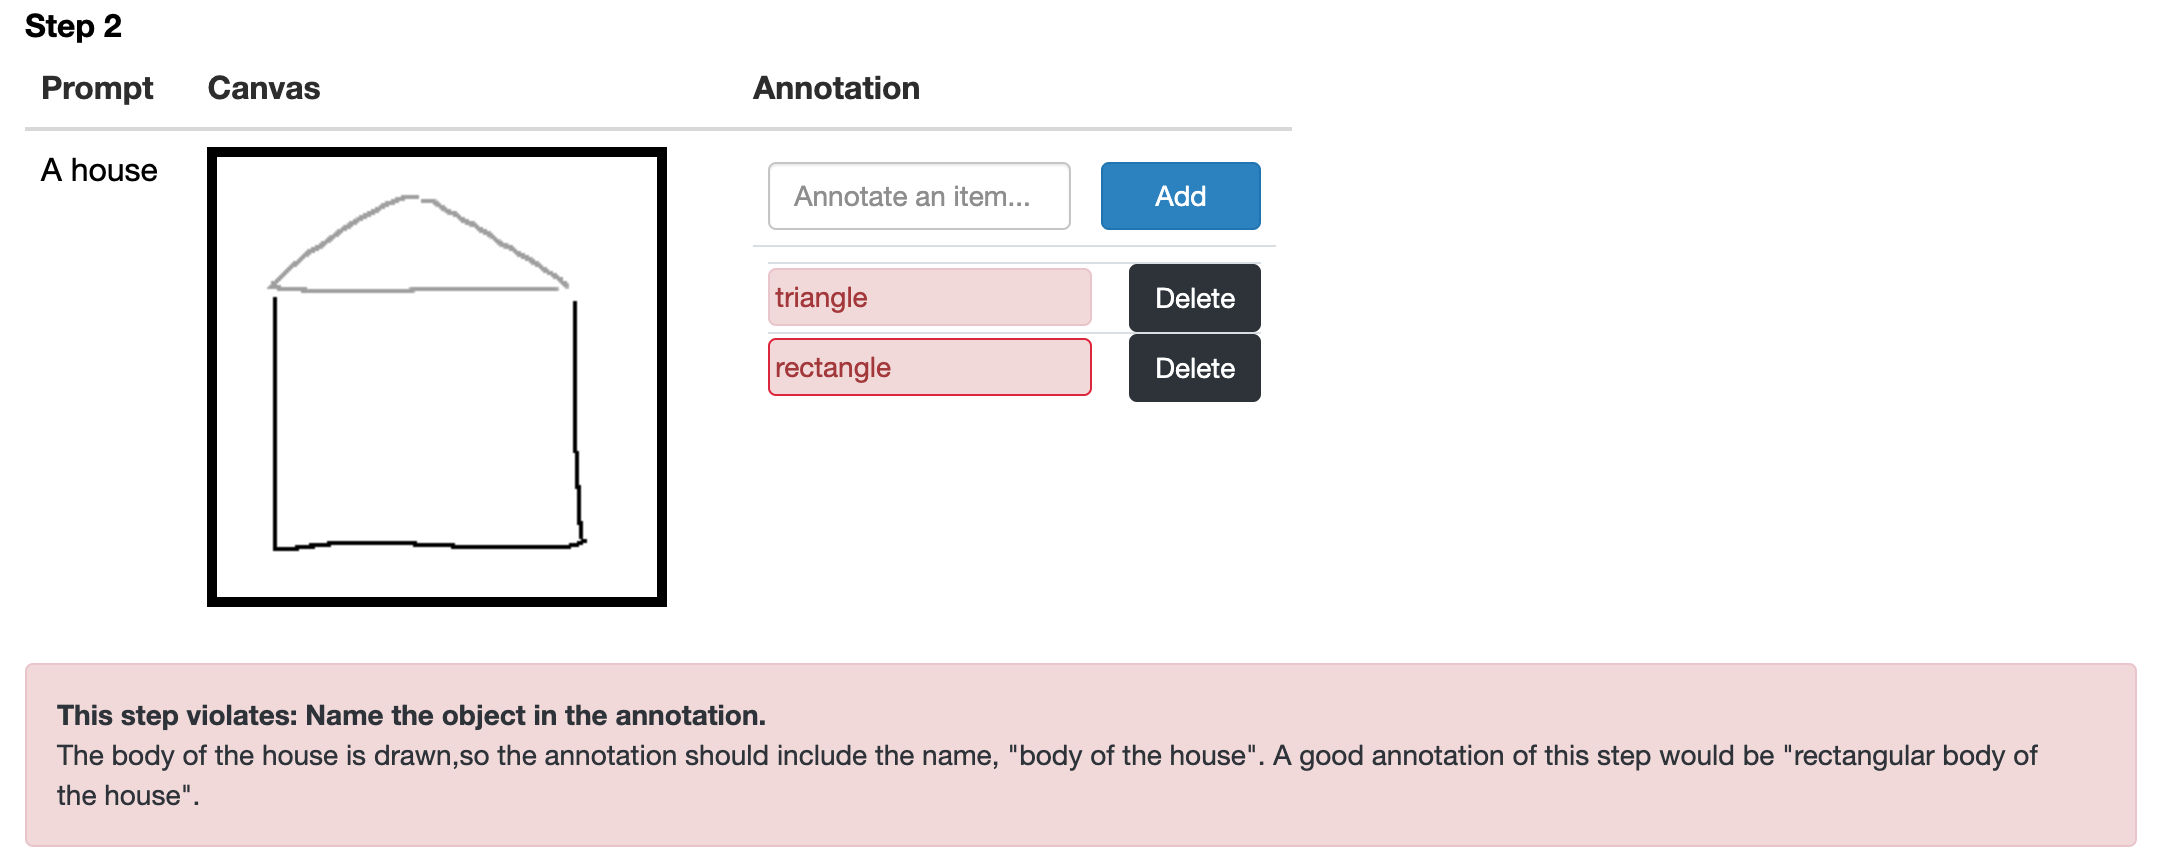
\includegraphics[width=.8\linewidth]{data_collection/v1_badeg_2.png}  
\end{subfigure}
\newline
\begin{subfigure}{\textwidth}
\centering
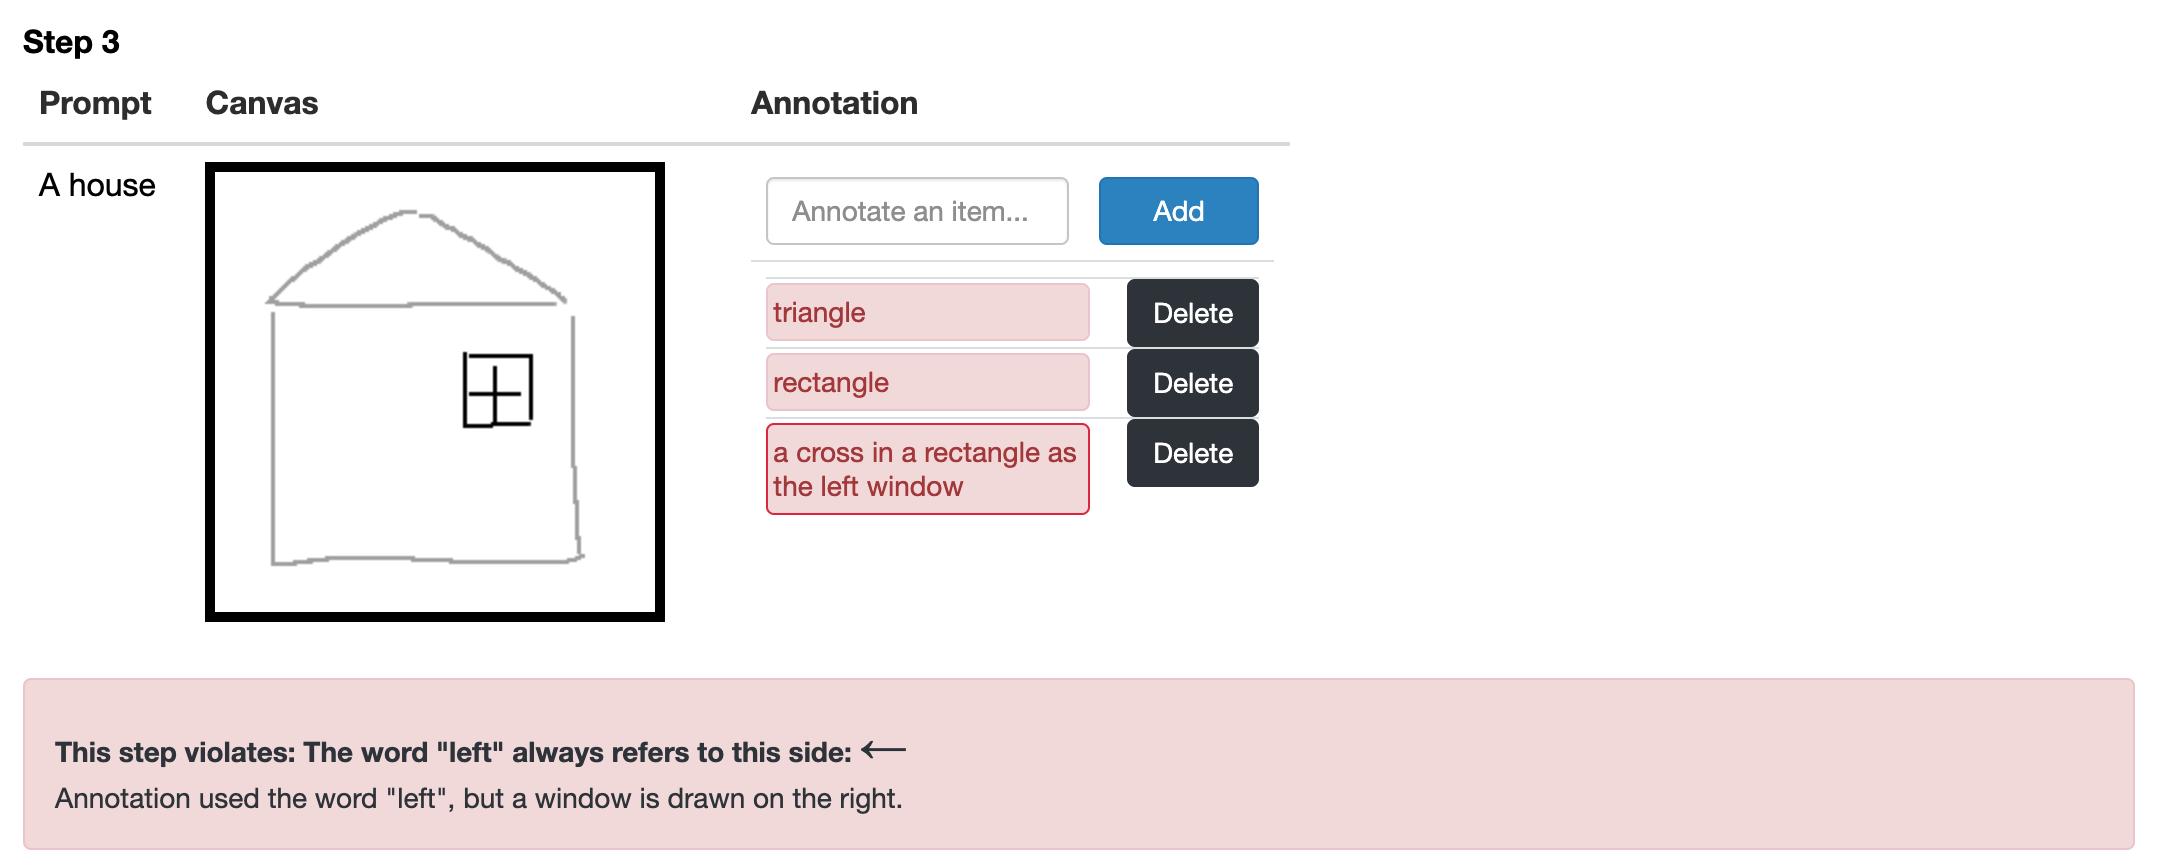
\includegraphics[width=.8\linewidth]{data_collection/v1_badeg_3.png}  
\end{subfigure}
\newline
\begin{subfigure}{\textwidth}
\centering
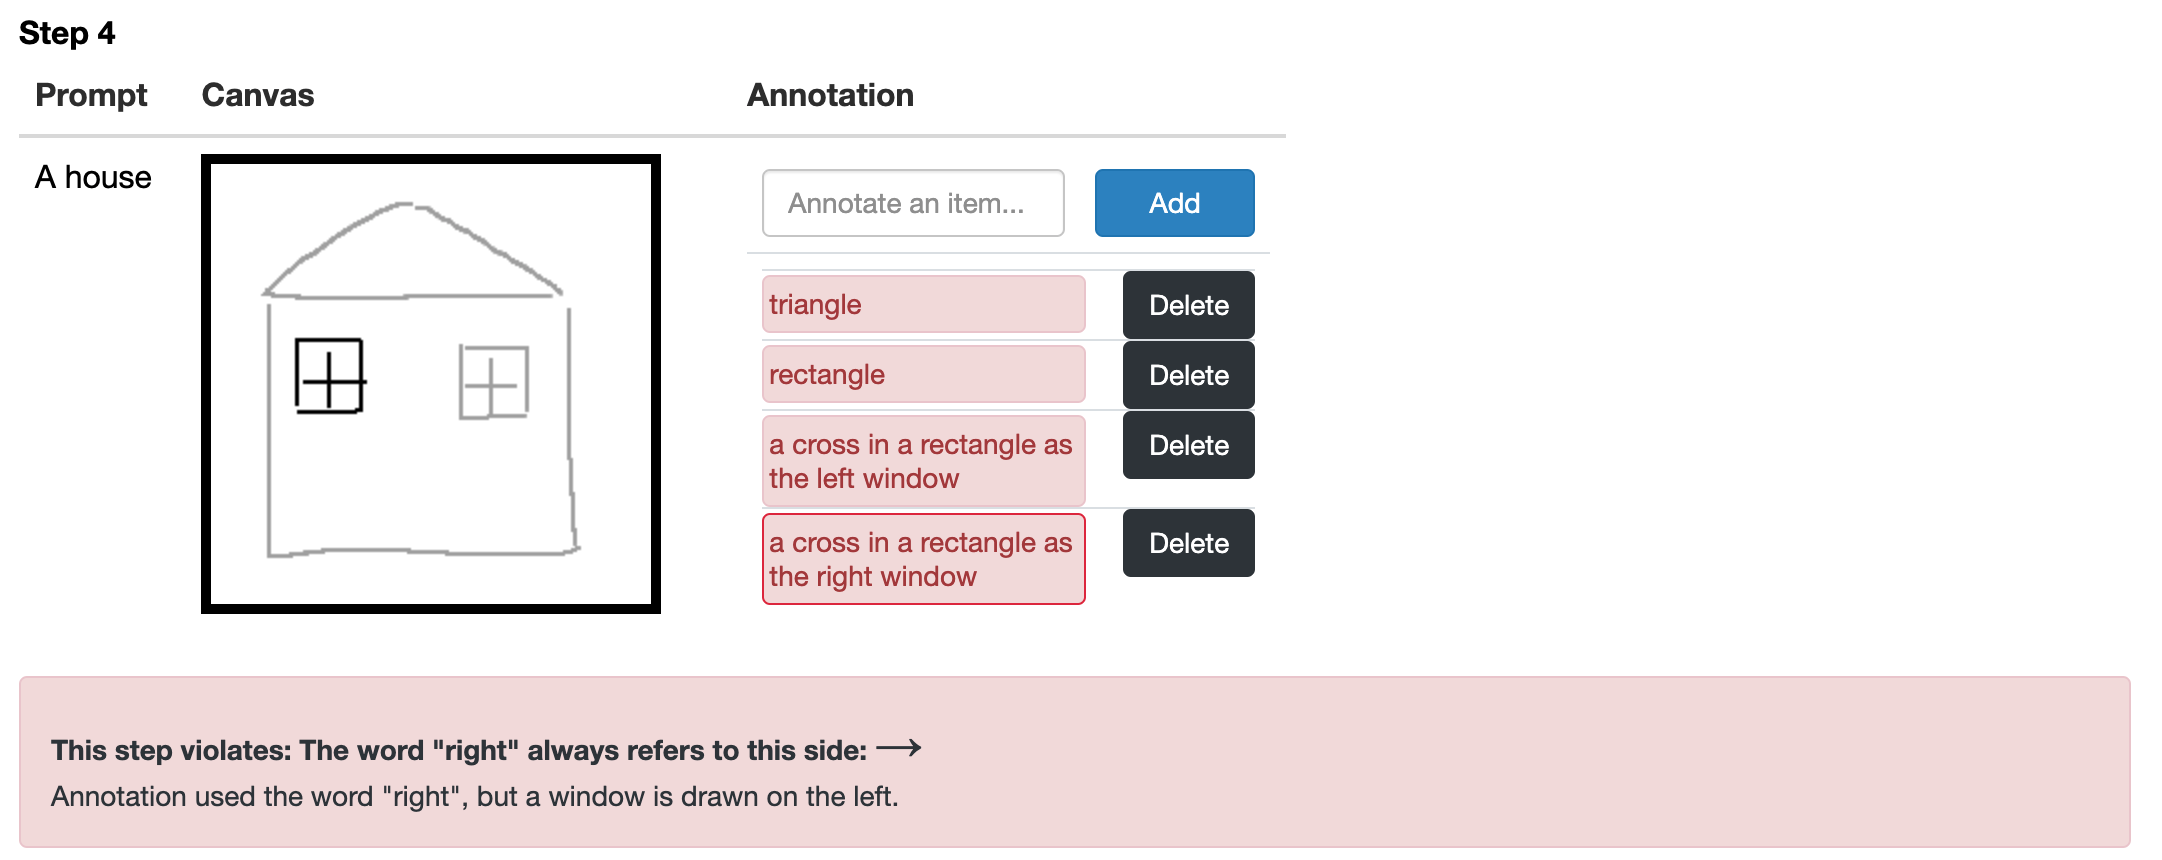
\includegraphics[width=.8\linewidth]{data_collection/v1_badeg_4.png}  
\end{subfigure}
\caption{Screenshots of an example in final version of the requirements in Version 1.}
\label{v1.badeg}
\end{figure*}

We also show \textcolor{red}{\underline{Bad Example 2}} in Figure \ref{v1.badeg} as an instance of the examples used in the final requirements. To view all the examples, refer to: \url{https://erinzhang1998.github.io/portfolio/amazon_anno}. 

\subsubsection{Qualification}

\begin{figure*}[!htb]
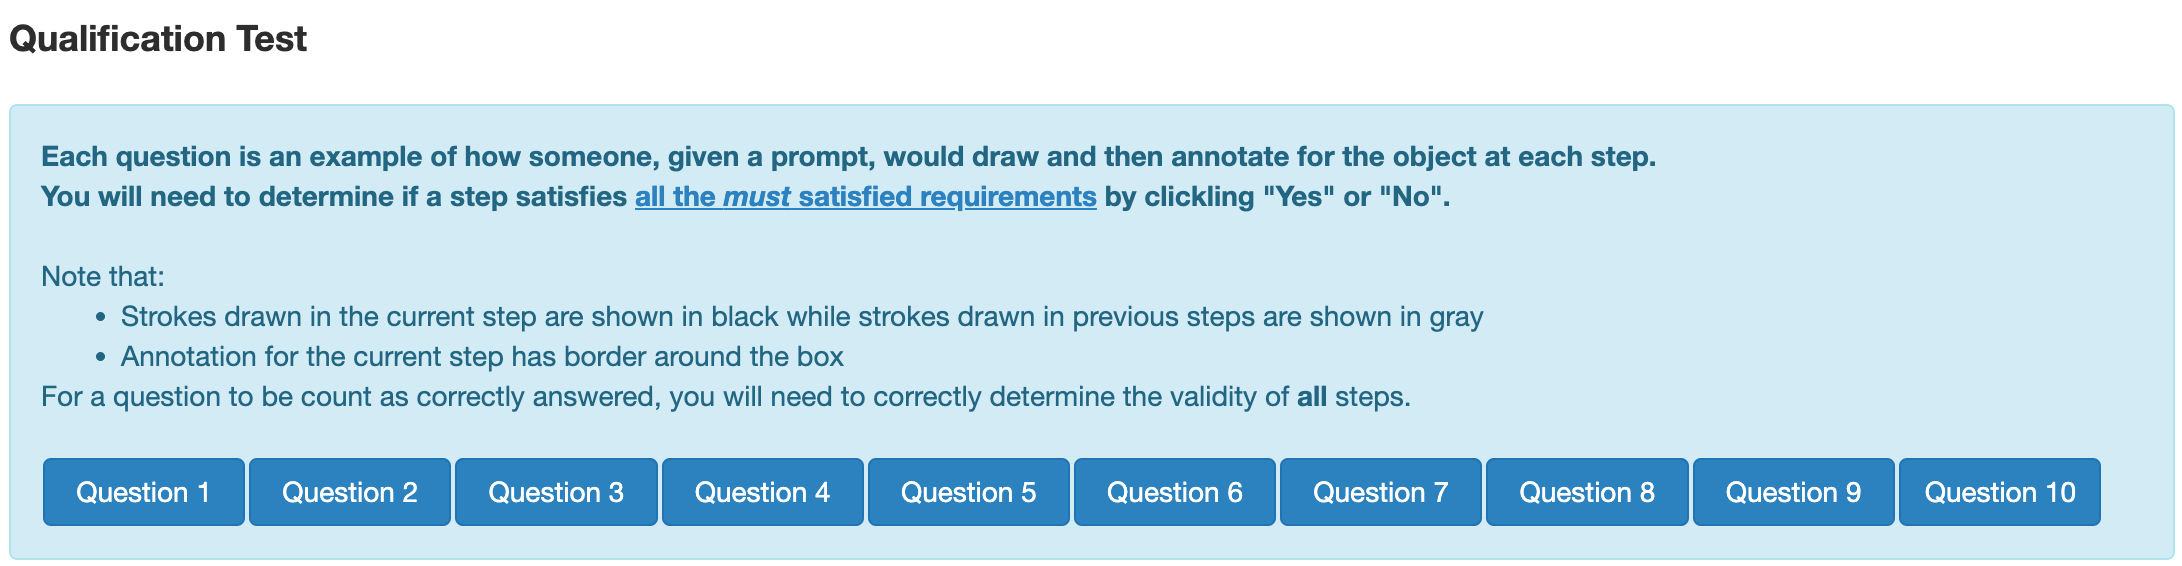
\includegraphics[width=\linewidth]{data_collection/v1_qual_header.png}  
\caption{Screenshots of the navigation bar in the qualification test of Version 1.}
\label{v1.qualification.nav}
\end{figure*}

\begin{figure*}[!htb]
\begin{subfigure}{\textwidth}
\centering
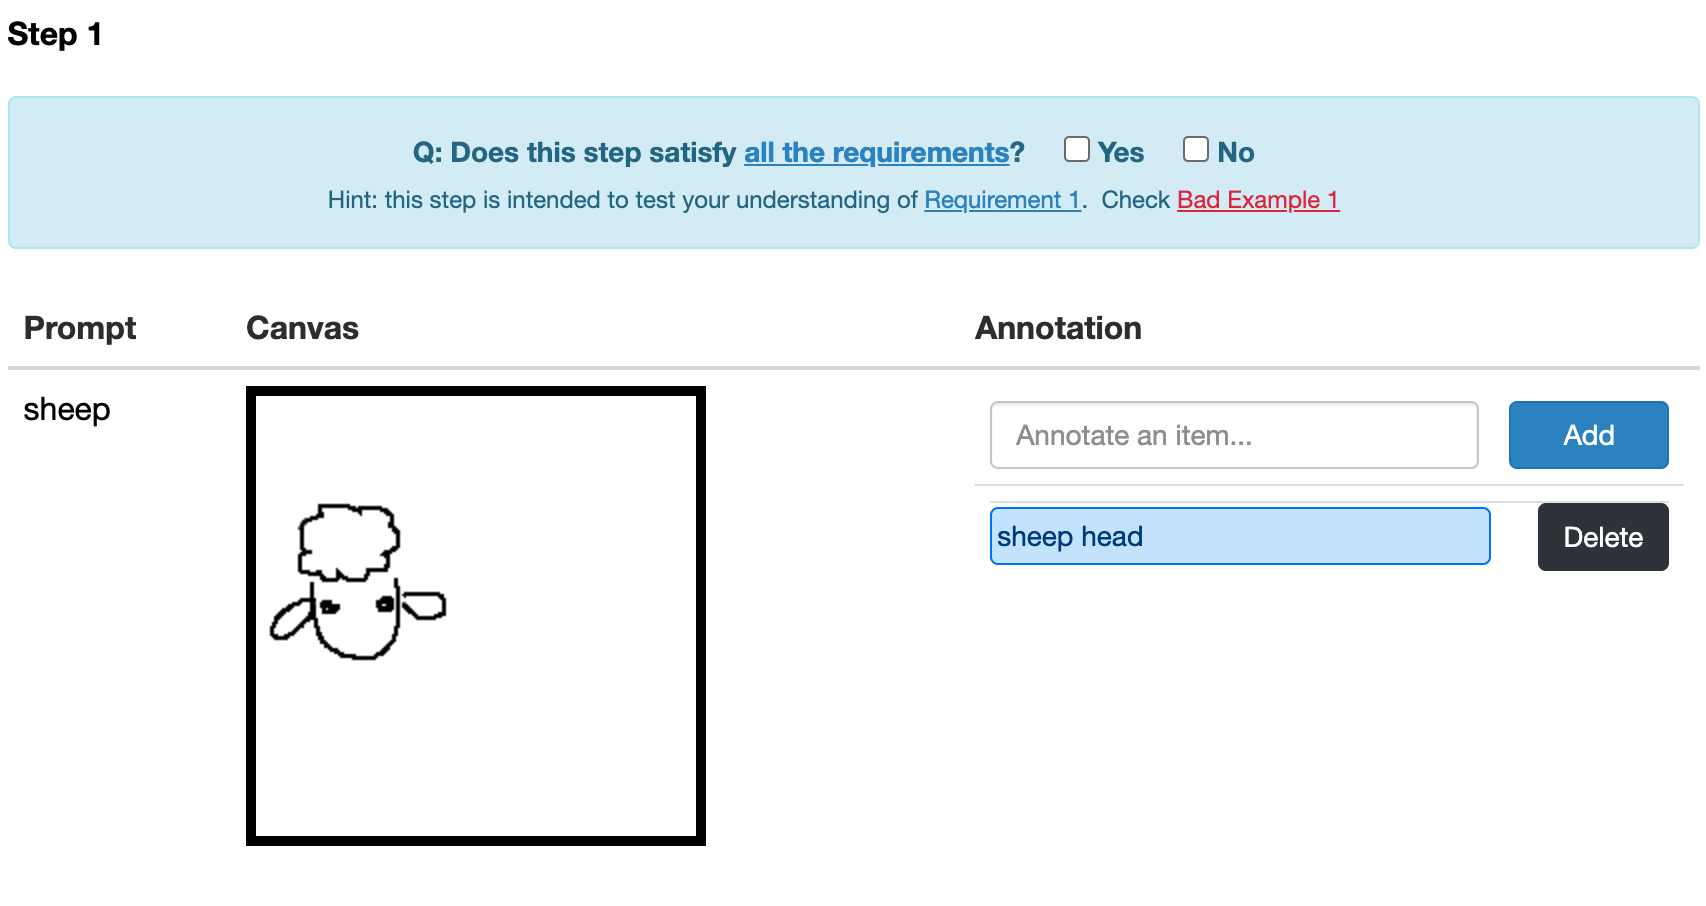
\includegraphics[width=.8\linewidth]{data_collection/v1_qual_q9_1.png}  
\end{subfigure}
\newline
\begin{subfigure}{\textwidth}
\centering
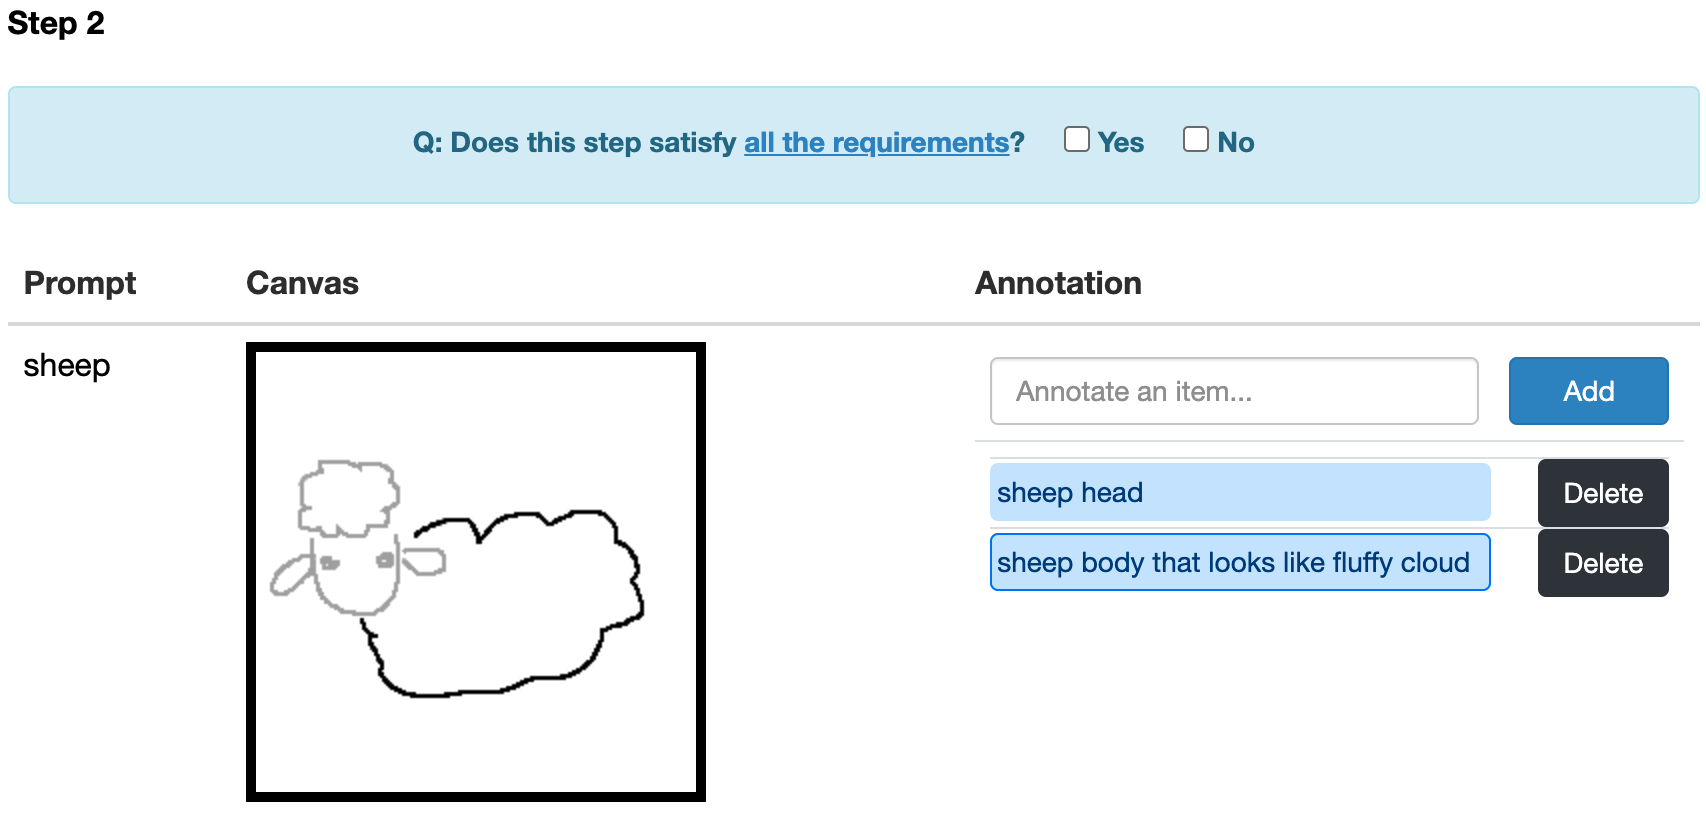
\includegraphics[width=.8\linewidth]{data_collection/v1_qual_q9_2.png}  
\end{subfigure}
\caption{Screenshots of question 9 in the qualification test of Version 1.}
\label{v1.qualification.q9}
\end{figure*}

We setup a qualification test on AMT to (1) train turkers to have better understanding of the task and (2) to select turkers who can provide annotations that satisfy all the requirements. Similar to the process of writing the requirements, we went through several rounds of testing with students in the lab to come up with a set of questions that have good correspondence with the requirements. The qualification test starts with the same instruction and requirements that will be used in the final HIT, thus allowing turkers to familiarize themselves with the requirements; moreover, this give them a chance to ask for clarifications before the final HIT. The test leads with a navigation bar (Figure \ref{v1.qualification.nav}) to make it convenient for turkers to switch between questions; originally, we displayed all questions in one page, but some people found it time-consuming to scroll from the later questions back up to the instructions, so we decided to display one question at a time. 
% We have refined the format of the qualification as we gathered feedback from people in the lab; we show a subset of the intermediate versions in Figure.
We show one question from the final qualification in Figure \ref{v1.qualification.q9}. We replicate the exact main task interface in the qualification test, and turkers need to determine whether every step of the mock annotation satisfies all the requirements; we also include hints on which requirement the question is testing for to encourage turkers to revisit the requirements and form better understanding of the task.  
To see the full test, refer to: \url{https://erinzhang1998.github.io/portfolio/amazon_qual}.

% [Figure x5: final qualification test]
%  At first, we asked the annotators to select which steps of the annotations satisfy the requirements (Figure x6.a); in order to use repetition to ensure deep understanding of the requirements, we changed to asking a yes/no question for every step, as shown in Figure x6.b.  

\subsection{Deployment Results}

% In order to determine how feasible the task is, we first deployed a version among lab members, and we obtained 55 drawings along with their annotations. All 55 drawings are shown in Figure v1.results.2. Some examples of step annotations are shown in Figure v1.results.3.  

% [Figure v1.results.2: 55 drawings from lab deployment (see jupyter notebook oct\_28\_trial\_analysis)]
% [Figure v1.results.3: 3 examples?]
To deploy our first pilot, we need to come up with a set of prompts that are in the forms of \textit{adjective}$\times$\textit{noun}. The list of adjectives includes: 
\textit{happy, sad, surprised, sleepy, lovestruck, evil};
% \textit{happy}, \textit{sad}, \textit{surprised},\textit{sleepy},\textit{lovestruck},\textit{evil}; 
the list of nouns includes: 
\textit{person, kid, cat, bear, dog, sheep, jellyfish, cup of boba, apple, burger, sun, moon, star}.
% \textit{person}, \textit{kid}, \textit{cat}, \textit{bear}, \textit{dog}, \textit{sheep}, \textit{jellyfish}, \textit{cup of boba}, \textit{apple}, \textit{burger}, \textit{sun}, \textit{moon}, \textit{star}. 
We hope to test what drawings and text descriptions annotators would provide for prompts that ask for imaginative beings not in this world, such as \textit{evil apple} or \textit{lovestruck moon}. Our first reason for doing so was that current text-to-image synthesis models, such as DALL-E and GPT-3, can produce creative artwork from abstract prompts that include novel compositions of unrelated concepts; we want to create a dataset that has the capacity to support learning models that can similarly respond to these imaginative prompts through interactive drawing. 
[!] Moreover, if we backtrack to version 0 for a second, the reason why we considered basic geometric shapes was because we are interested in how humans are able to transfer the usage of a circle to different context: a large circle could be a face, an eye, a big piece of cherry, or a moon, so transferring the same visual concept to different sketches. Also there is an aspect of transferring the same language to different context, such as in what ways the adjectives demonstrate the same concept across different object and in what ways they adapt and show different visual qualities when used on different objects.   
% The compositional nature of language allows us to put together concepts to describe both real and imaginary things. We find that DALL·E also has the ability to combine disparate ideas to synthesize objects, some of which are unlikely to exist in the real world. We explore this ability in two instances: transferring qualities from various concepts to animals, and designing products by taking inspiration from unrelated concepts.

[Figure v1.results.4: drawings from the amt pilot]

What surprised us was the amount of time turkers spent on the task. Histograms of time each annotator spent on the task is illustrated in Figure v1.results.1. Statistics of the distributions are shown in Table v1.results.1. The discrepancy might be caused by the fact that lab members with their background in computer science have an implicit understandings of what kind of quality data are needed to train ML models.   

[Figure v1.results.1: a: oct 28 lab deployment. b: dec 28 amt deployment]
[Table v1.results.1: comparing the statistics of lab vs. amt deployment]

In violation of DQ \ref{data_design_1}. Drawing does not illustrate the prompt well. The quality of the drawings are greatly influenced by how well the annotator can understand the prompts. Drawing is by its nature very subjective, so when we were examining through the sketches that we collected, we were not able to understand in what ways some sketches convey the prompts. 
[Figure v1.results.4: some examples of sketches that cannot illustrate the prompt from our perspective]

In violation of DQ \ref{data_design_2} and \ref{data_design_3}. Another problem was that annotators often fail to describe every parts they drew in one step, or the descriptions miss some parts in the step, or the description does not align well with the drawings.   
[Figure v1.results.5: some examples of mis-aligned descriptions]

\section{Contrastive Sketch Text Dataset} \label{datav2}

\subsection{Overview}
In response to the pilot results, we reconsider the data collection pipeline. 
We examined existing sketch datasets to see how their annotations could facilitate our data collection (dataset details are explained in Section \ref{relatedWorkChapter}).    
To shorten the time spent on sketching, we no longer asked annotators to sketch and instead only asked them to describe sketches in the QuickDraw dataset. 
Although we could no longer design text prompts ourselves and collect creative sketches like the ones in the previous pilot, we solved the problem that it was difficult to understand how some sketches illustrated the given prompts. 

The most important objective that this dataset should fulfill is allowing us to study how sketches share similar semantic parts and descriptions that are adapted to be used for different objects. We must resolve the issue that some text descriptions in the pilot do not match the drawing.  
% To solve this problem of misaligned text descriptions and drawings, 
Therefore, we use semantic part annotations from the Sketch Perceptual Grouping (SPG) dataset, which provides semantic part labels for each stroke in $20,000$ sketches from the QuickDraw dataset. In this way, annotators did not need to spend time thinking about how to segment sketches into parts themselves. 
Moreover, to help annotators coming up with creative ways to describe the semantic parts, in each task, we present a pair of sketches with contrasting features, implicitly priming them to describe the visual differences. (Note that all sketches in figures from this section on come from the QuickDraw dataset \citep{ha2017neural}.)
% Between  and SketchSeg, both containing annotaiton for semantically meaningful parts in sketches, 
% SPG annotates for QuickDraw sketches while SketchSeg collects its own sketches. We picked SPG, since it will be easier in the future to extend our datasets given the large QuickDraw reservoir of sketches. 
% Moreover, SketchSeg dataset contains a \textit{fourleg} category that includes many different kinds of animals, such as horse, sheep, and cow, but the QuickDraw categories are more fine-grained, so form a model learning perspective, SPG will also be more generalizable.  

\subsection{Interface Design}


\subsubsection{Main Task Interface}
When collecting the previous prompt-guided dataset, we relied on testing the interface with students in the lab to determine our design, but we observed performance differences between the students and turkers, such as amount of variety in the sketches, amount of time spent on the task, and common confusions related to understanding the requirements. 
Therefore, when collecting the contrasting sketch text dataset, we deployed several pilots on AMT to design the new interface.  
In Figure \ref{v2.main_task.1}, we show how the main task interface progressed from the first pilot to the final version used to collect the entire dataset. 

To better study how similar words are used differently across sketches, we changed to collect adjective phrases (Figure \ref{v2.main_task.1.b}, \ref{v2.main_task.1.d}) from collecting whole sentences (Figure \ref{v2.main_task.1.a}).  
We juxtaposed two sketches and highlighted the parts to be annotated in different colors to help annotators notice the contrasting features. 
Moreover, this design expedited the annotation process, since it was easier for people to perform contrasting tasks than to generate descriptions from a single sketch. 

\begin{figure*}[!h]
\begin{subfigure}{\textwidth}
\centering
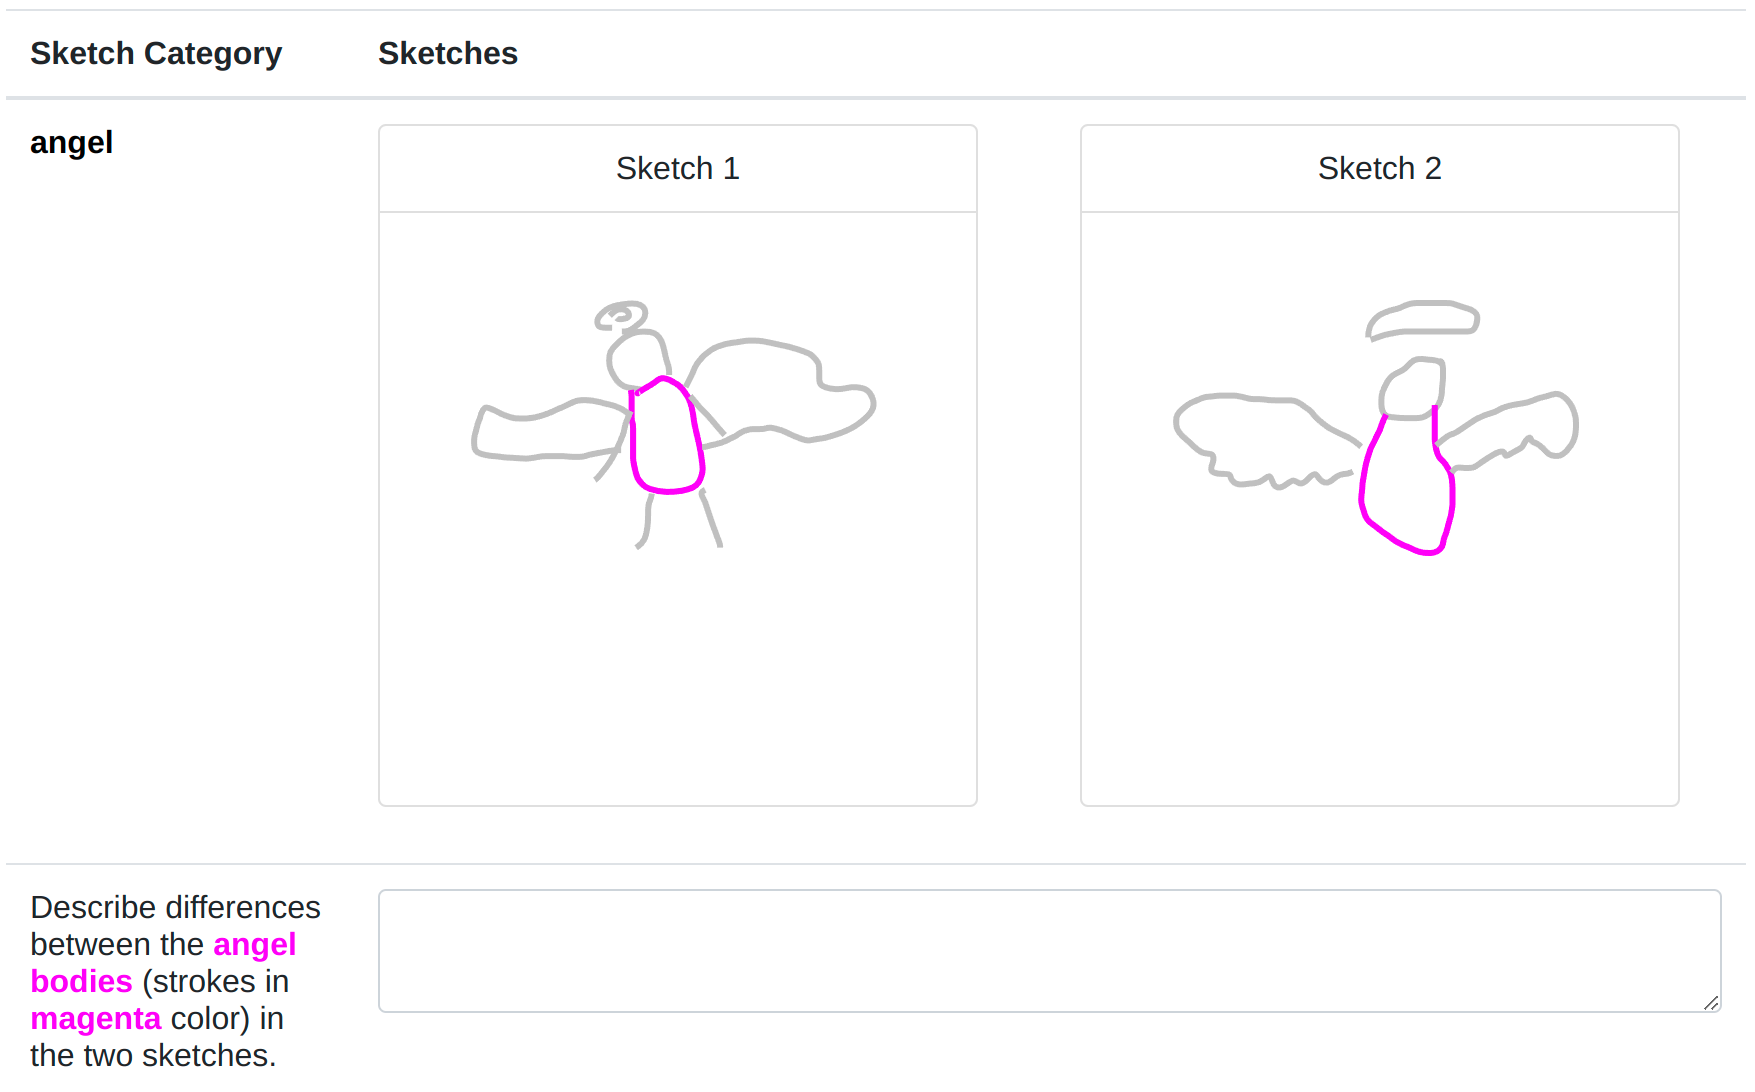
\includegraphics[width=.8\linewidth]{data_collection/version2/v2annofeb1.png}  
\caption{In the first pilot, we ask annotators to describe differences between the two sketches in full sentence.}
\label{v2.main_task.1.a}
\end{subfigure}
\newline
\begin{subfigure}{\textwidth}
\centering
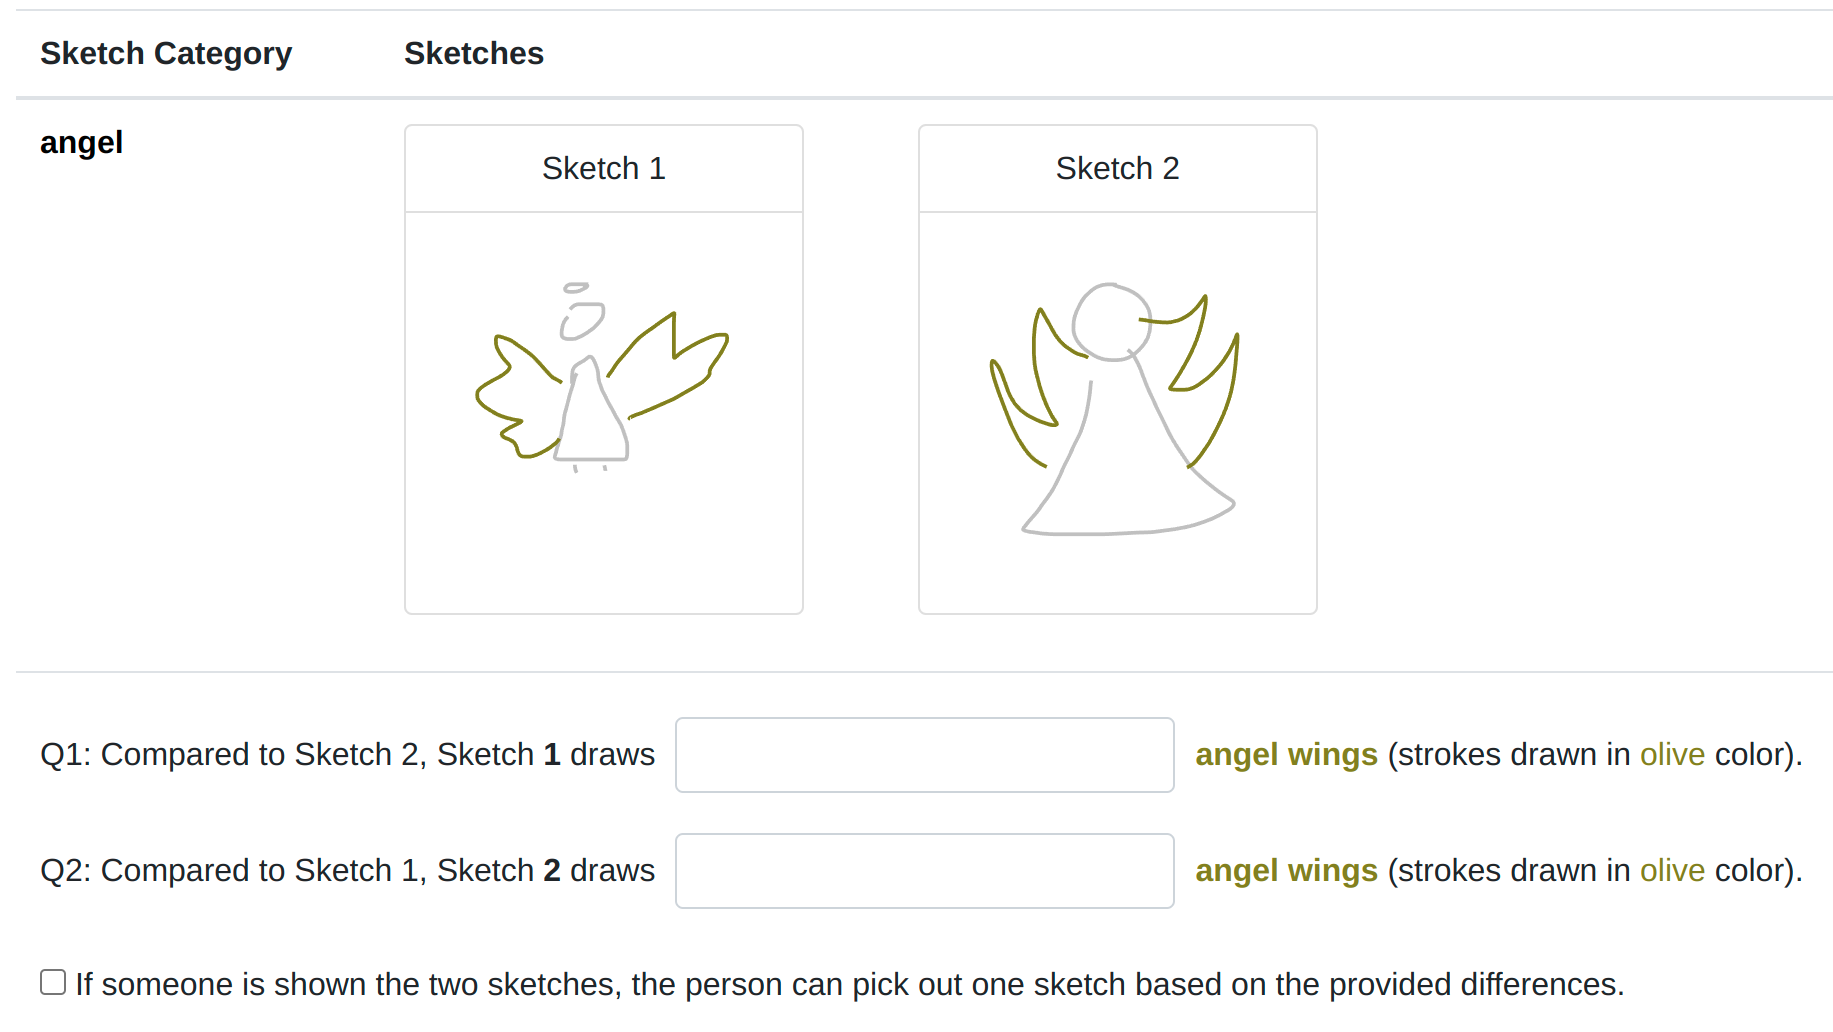
\includegraphics[width=.8\linewidth]{data_collection/version2/v2annofeb4.png}  
\caption{Compared to the previous pilot (\ref{v2.main_task.1.a}), we still ask explicitly the differences between the sketches but limit annotations to adjective phrases.}
\label{v2.main_task.1.b}
\end{subfigure}
\end{figure*}
  
\begin{figure*}[!h]
\ContinuedFloat
% \begin{subfigure}{\textwidth}
% \centering
% 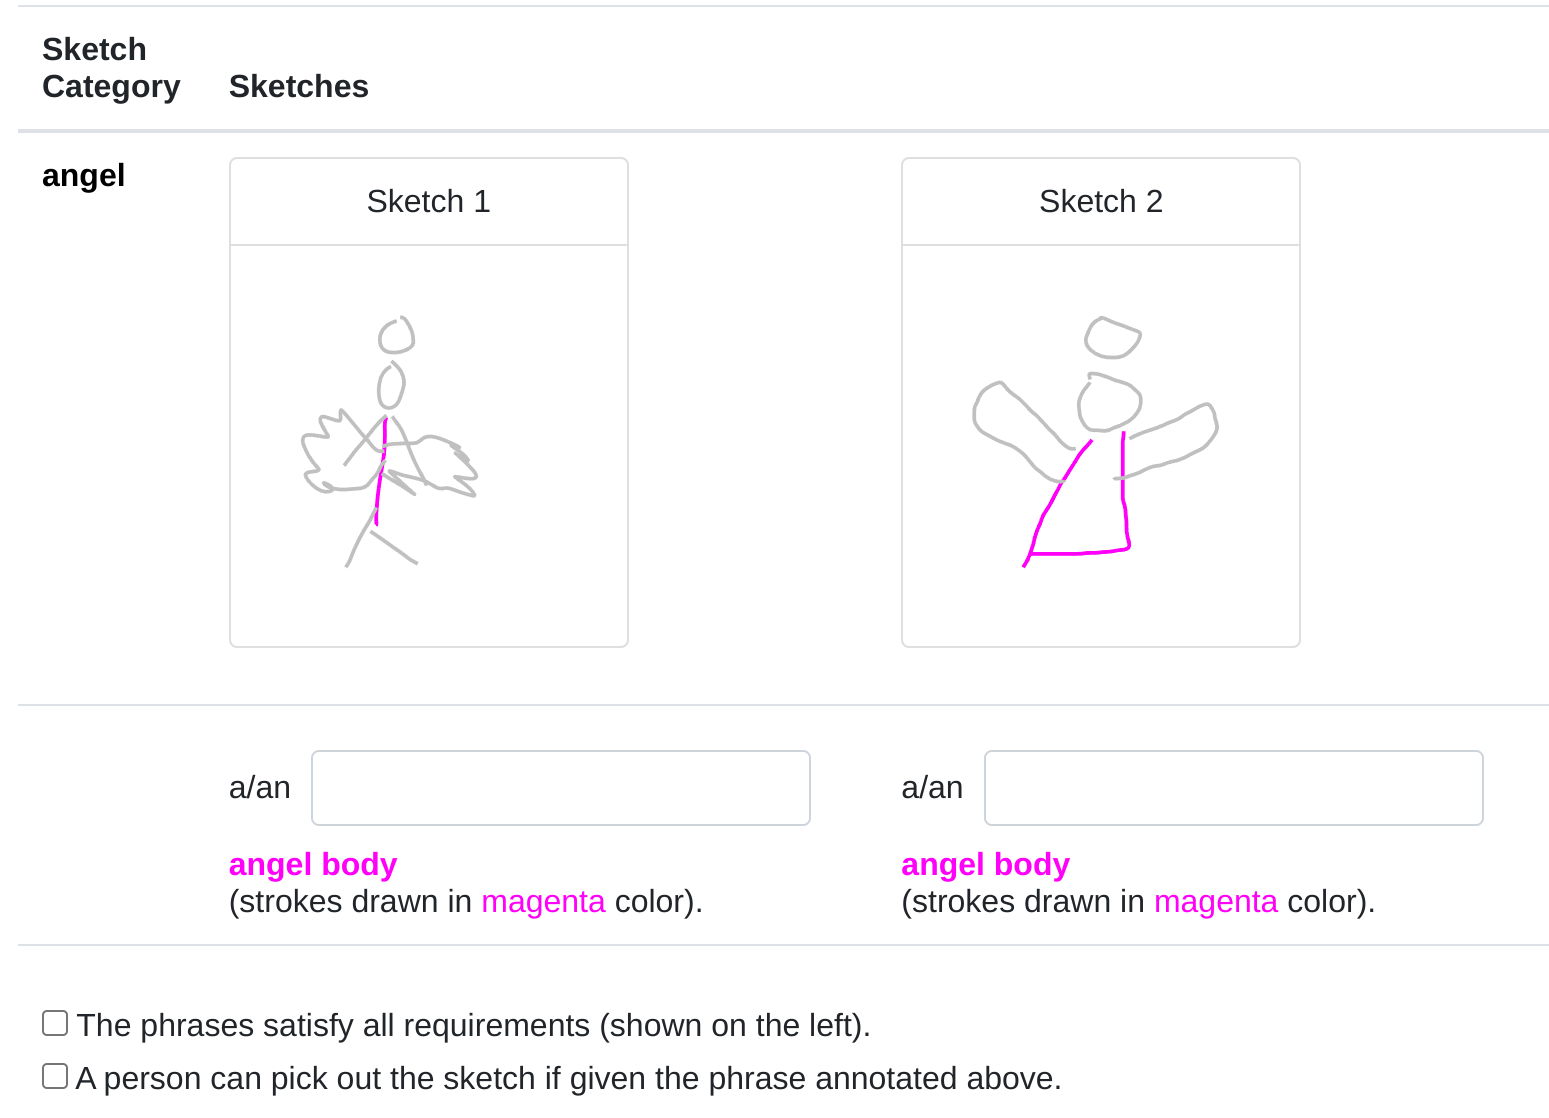
\includegraphics[width=.8\linewidth]{data_collection/version2/v2annofeb8.png}  
% \caption{Design of main task for third pilot.}
% \label{v2.main_task.1.c}
% \end{subfigure}
% \newline
\begin{subfigure}{\textwidth}
\centering
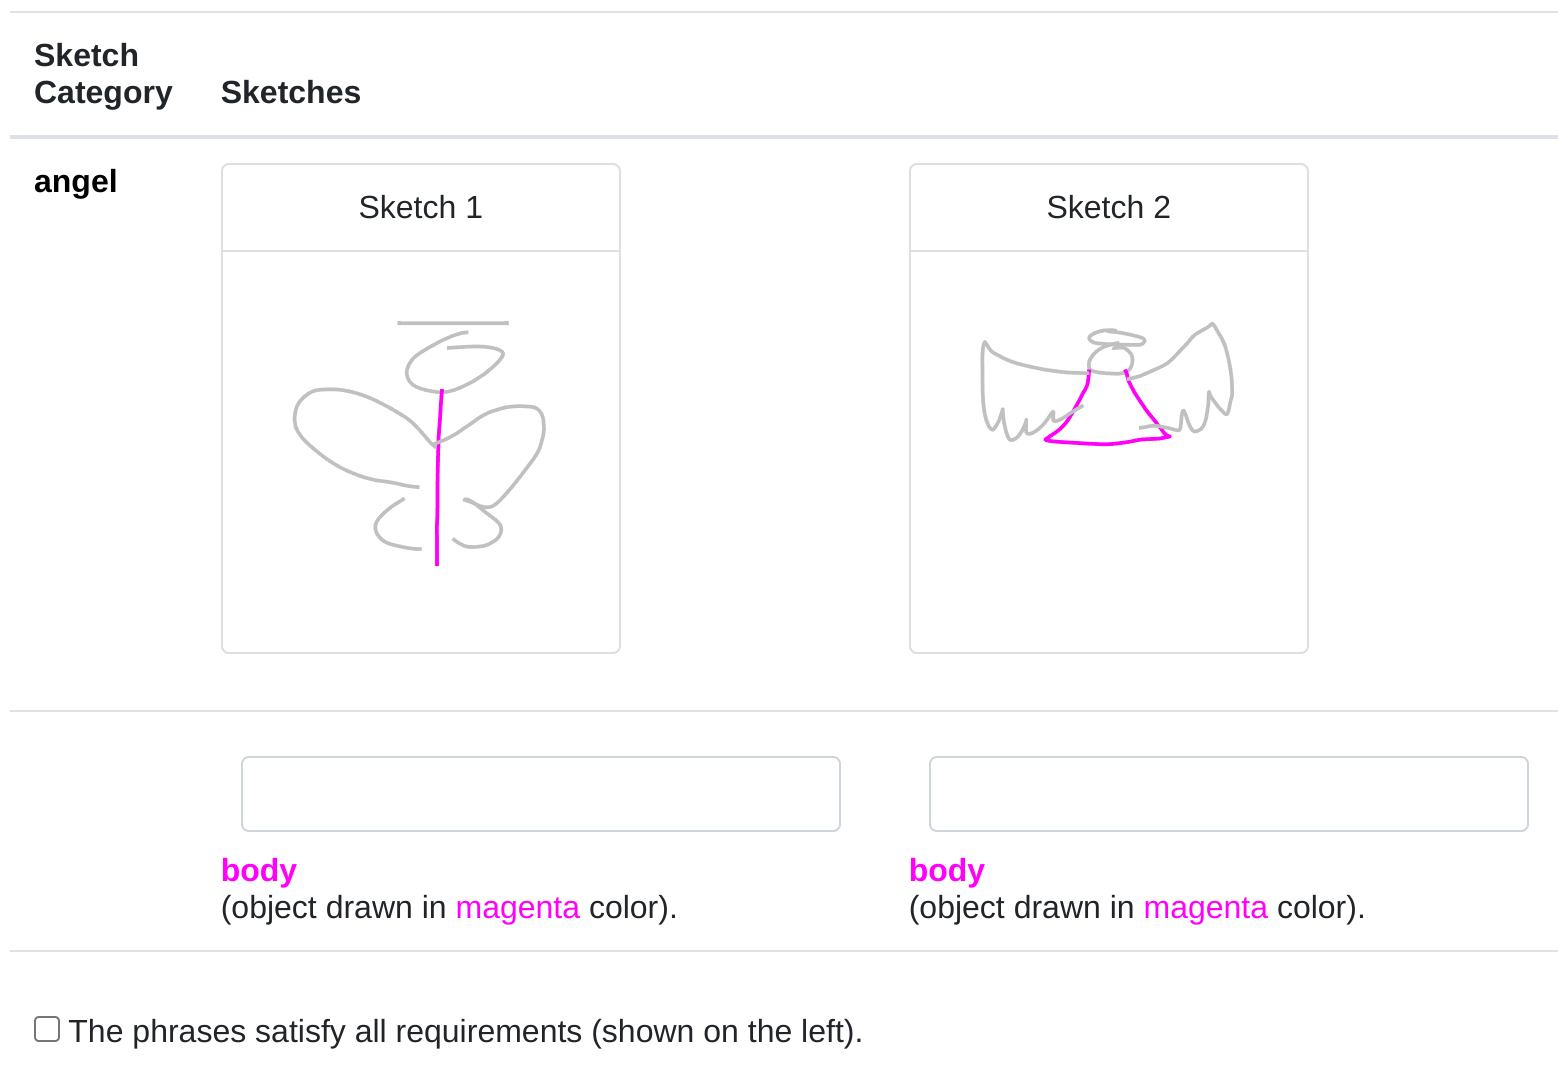
\includegraphics[width=.8\linewidth]{data_collection/version2/v2anno.png}  
\caption{Similar to the last pilot (\ref{v2.main_task.1.b}), the final version asks for adjective phrases, but we do not state explicitly that annotators should describe the visual differences to allow for more creativity.}
\label{v2.main_task.1.d}
\end{subfigure}
\caption{Different versions of the main task interface in chronological order. Final version used to collect the entire dataset is \ref{v2.main_task.1.d}.}
\label{v2.main_task.1}
\end{figure*}

We chose the contrasting pairs by rendering each part in the sketches and encode the parts into image features using CLIP. For every part type, we iterate through the features and pair features that are the most distinct in terms of cosine distance. For example, to select a pair of sketches with contrasting \textit{body}, we render the strokes that depict the \textit{body} in all angel sketches; all these angel body sketches are encoded by CLIP, and pairs of bodies that are the most distinct are presented to the annotators in the format shown in Figure \ref{v2.main_task.1.d}.  
  
% At the beginning, we stated explicitly that annotators should describe the differences between the sketches (\textit{Describe differences} in \ref{v2.main_task.1.a} and \textit{Compared to Sketch 1/2} in \ref{v2.main_task.1.b}), but we received many annotations that contain comparative and superlatives, so we eventually only have a blank without any introductory phrases to overly emphasize that the goal of the tasks is to create a dataset of contrastive pairs of descriptions, and the juxtaposition is meant only as a mental hint to ease annotation.

\subsubsection{Instruction and Requirement}

\begin{figure*}[!h]
\centering
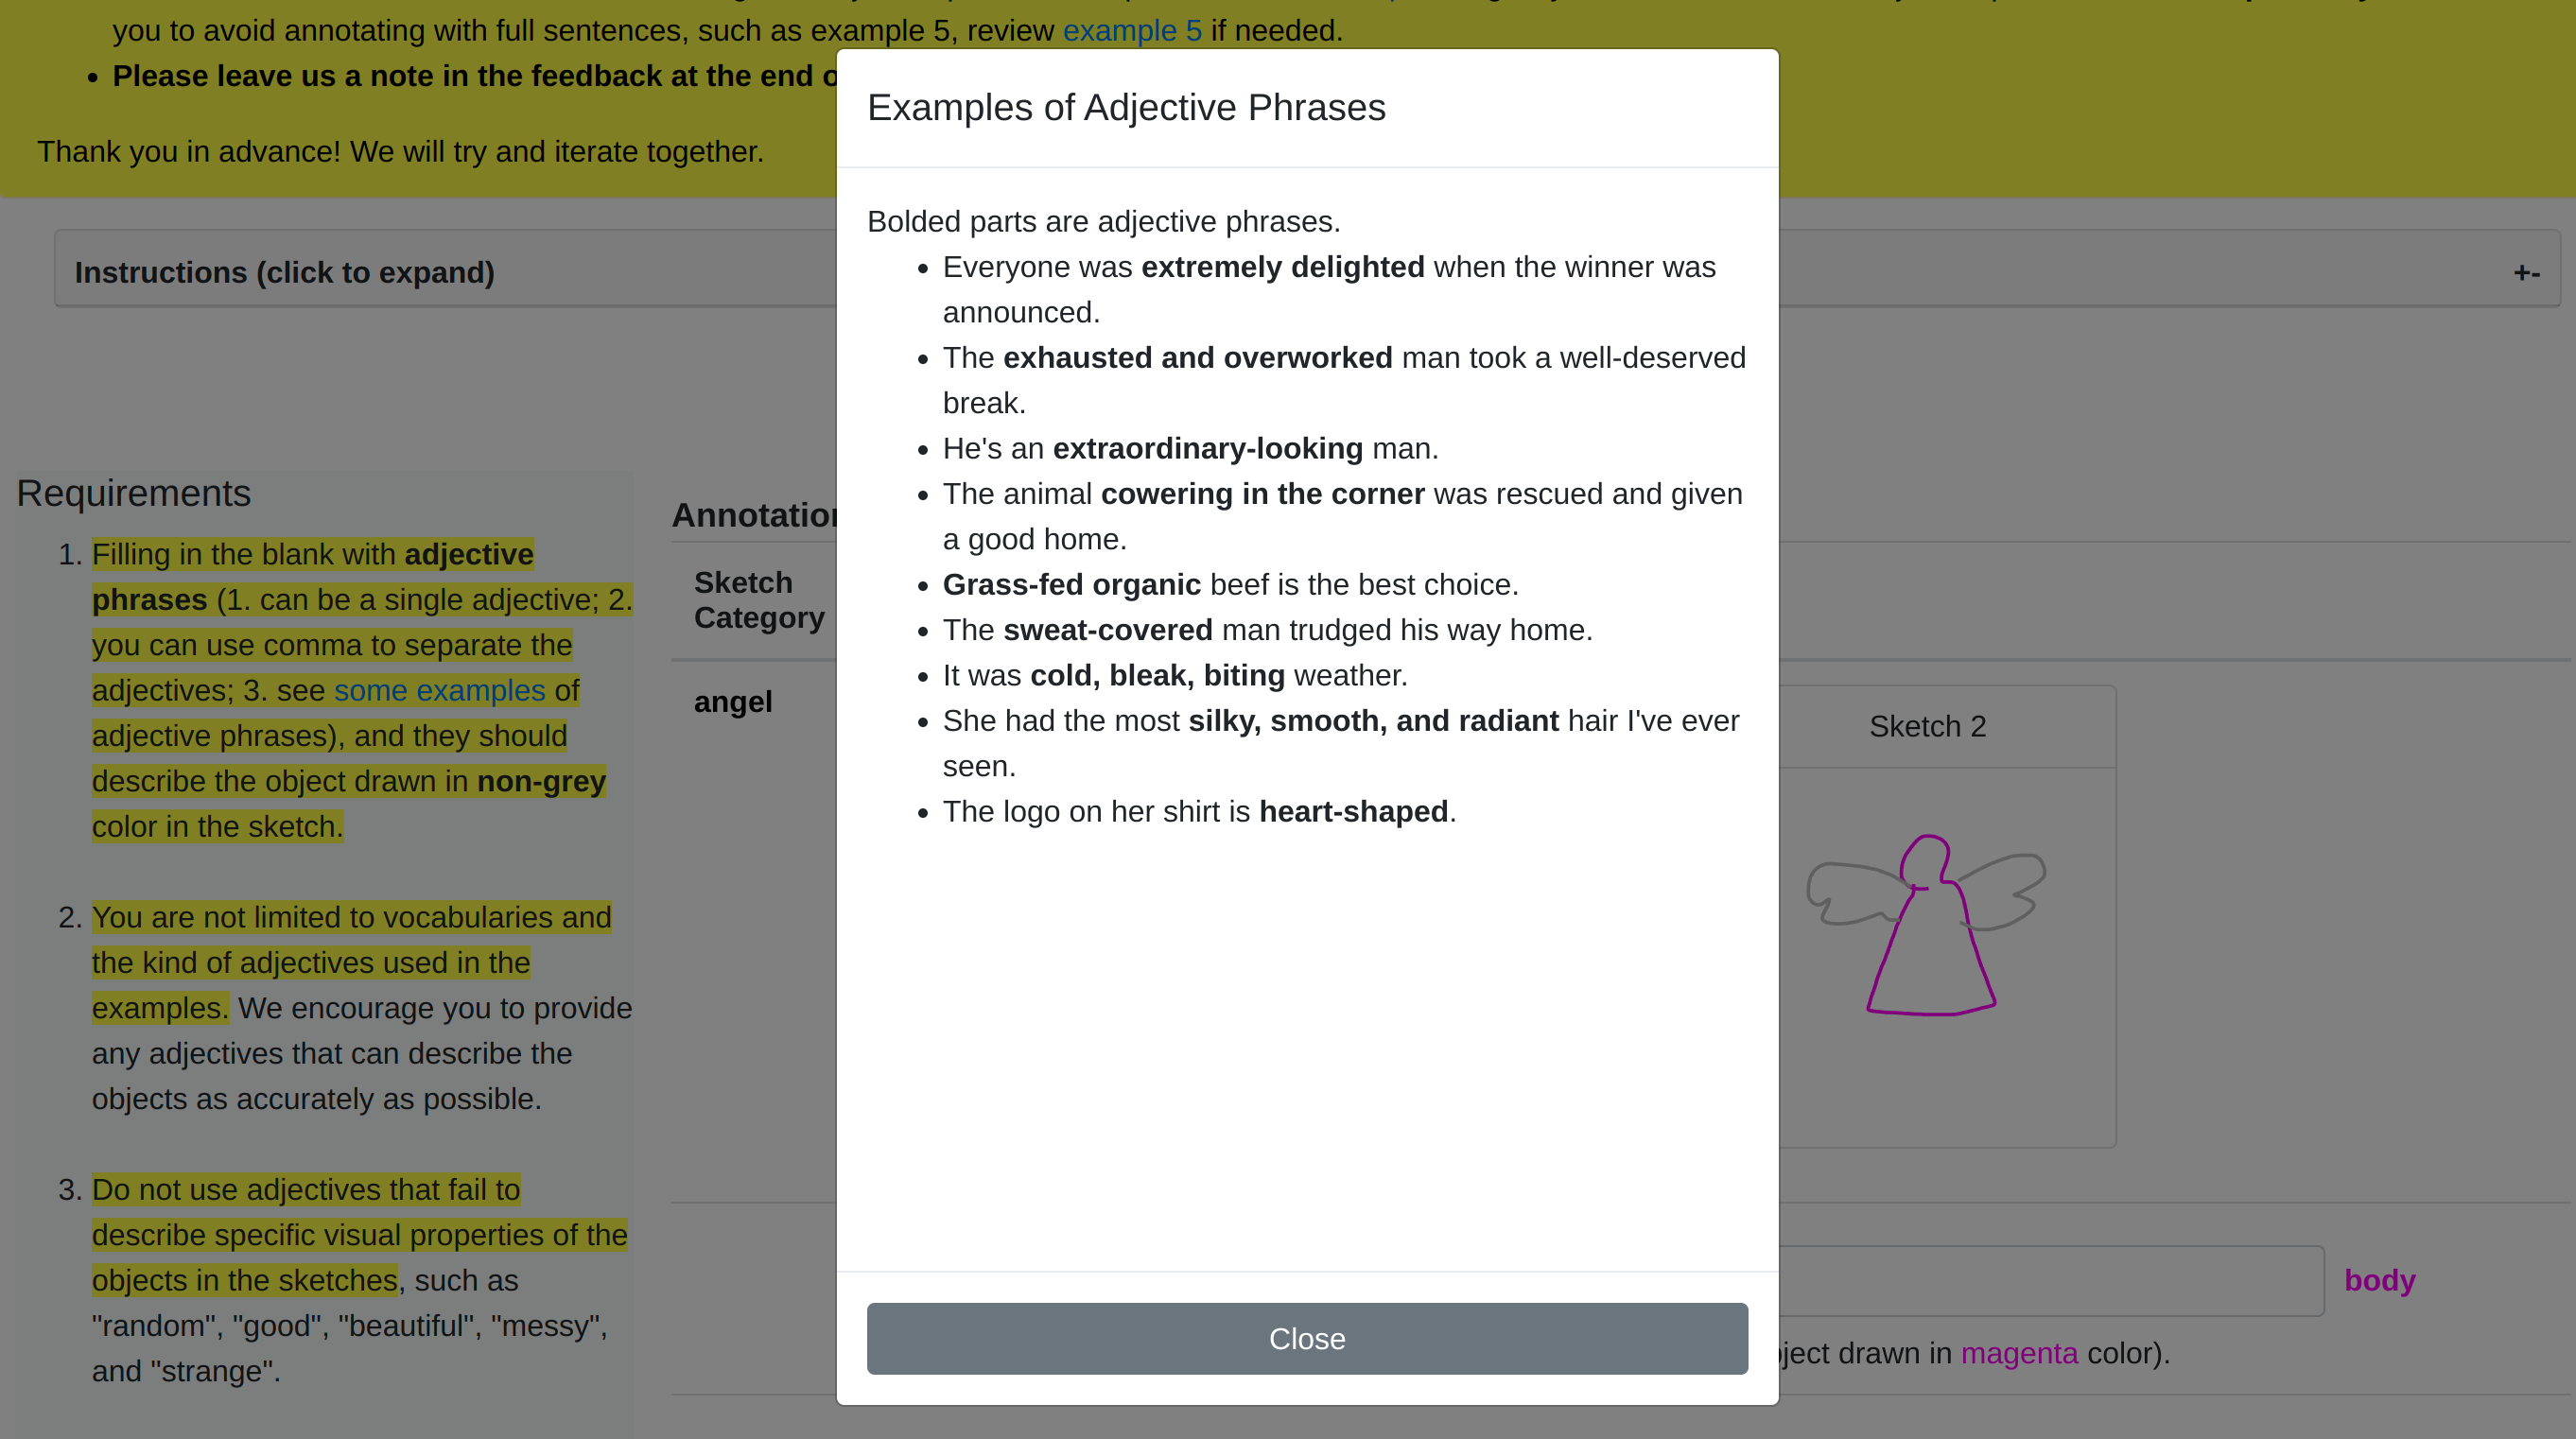
\includegraphics[width=\linewidth]{data_collection/version2/v2annoPop.png}  
\caption{A pop-up window containing examples of adjective phrases, used in collecting contrasting sketch text dataset in Section \ref{datav2}. It can be opened from the side panel by clicking on \textcolor{blue}{\it{some examples}}. Note that we used examples that are unrelated to our task on purpose, because annotators tended to repeat words in examples, so we tried to not bias them.}
\label{v2.adjective.phrases}
\end{figure*}

At the beginning, the instruction limited the annotators to provide three types of descriptions: shape, size, and position. 
However, in order to collect creative descriptions, we lifted restrictions on the type of words and only required annotators to fill in the blank with adjective phrases. We also provided some examples of adjective phrases in common sentences, unrelated to our task, for annotators to better understand their usage (Figure \ref{v2.adjective.phrases}). 

Since we simplified the HIT from 3 sub-tasks, sketching for the prompt, segmenting the sketches, and describing each step, to only asking for part descriptions, the requirements are much easier to write. 
We received less feedback from the annotators on being confused about the kind of sketches we wanted and the definition of semantic parts, which are now automatically highlighted in the sketches.   

\begin{figure*}[!h]
\centering
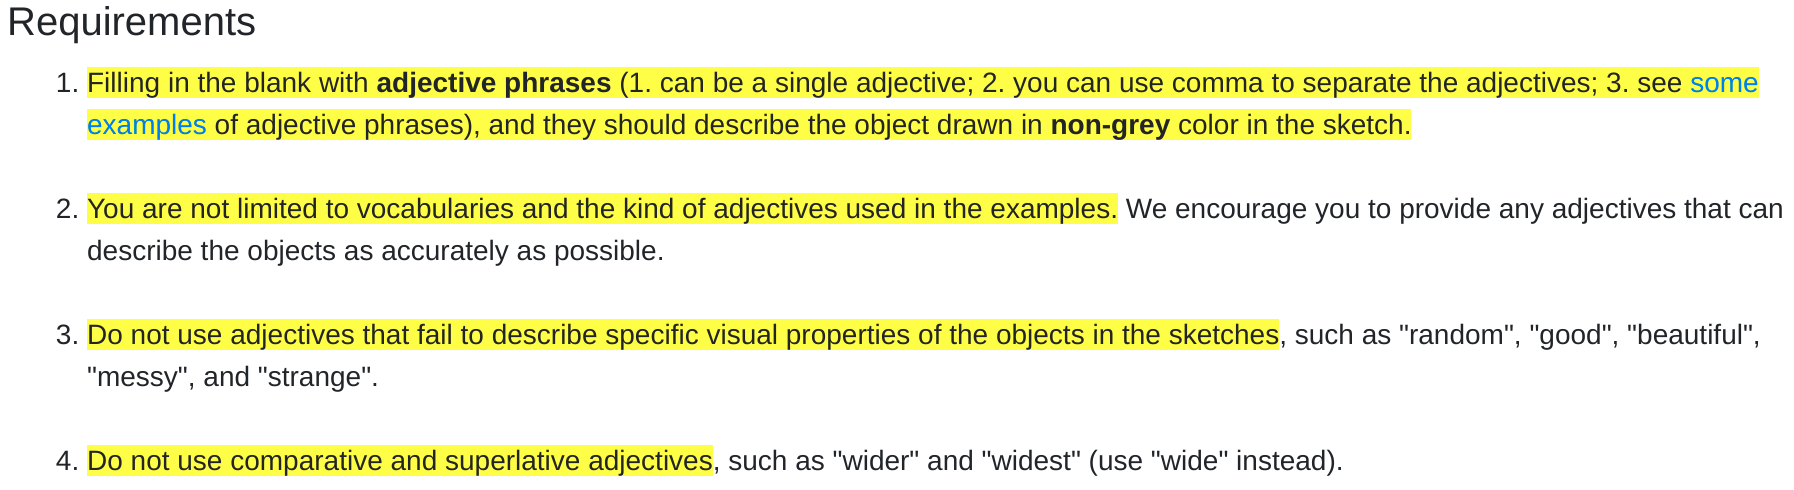
\includegraphics[width=\linewidth]{data_collection/version2/v2requirement.png}  
\caption{Requirements used in collecting the contrasting sketch text dataset (Section \ref{datav2}).}
\label{v2.requirement.1}
\end{figure*}

\begin{figure*}[!h]
\begin{subfigure}{\textwidth}
  \centering
  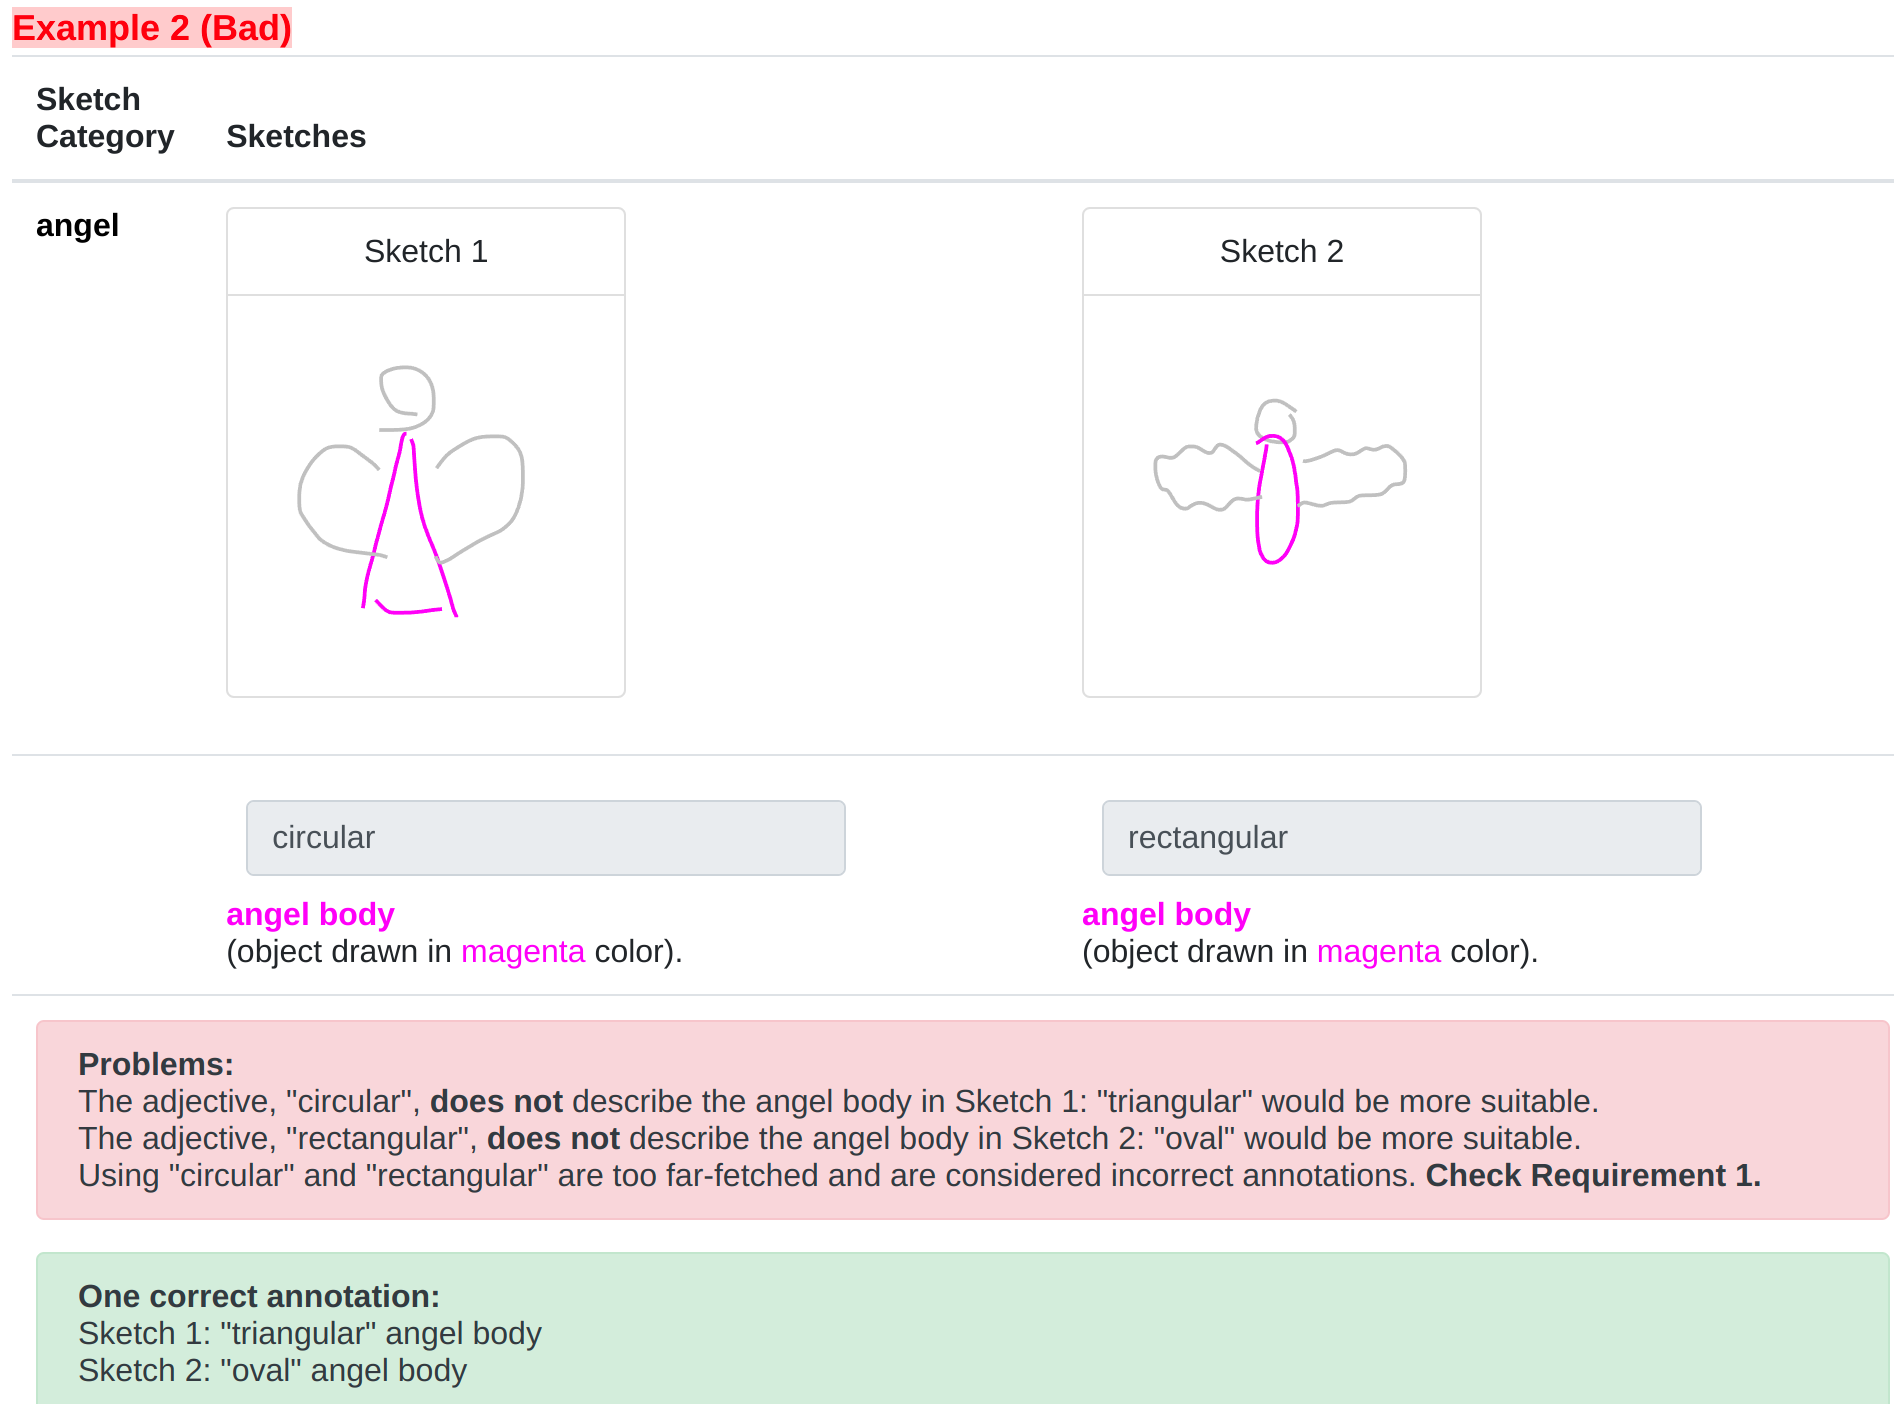
\includegraphics[width=0.8\linewidth]{data_collection/version2/v2example2.png}  
\end{subfigure}
\newline
\vspace{5mm}
\begin{subfigure}{\textwidth}
  \centering
  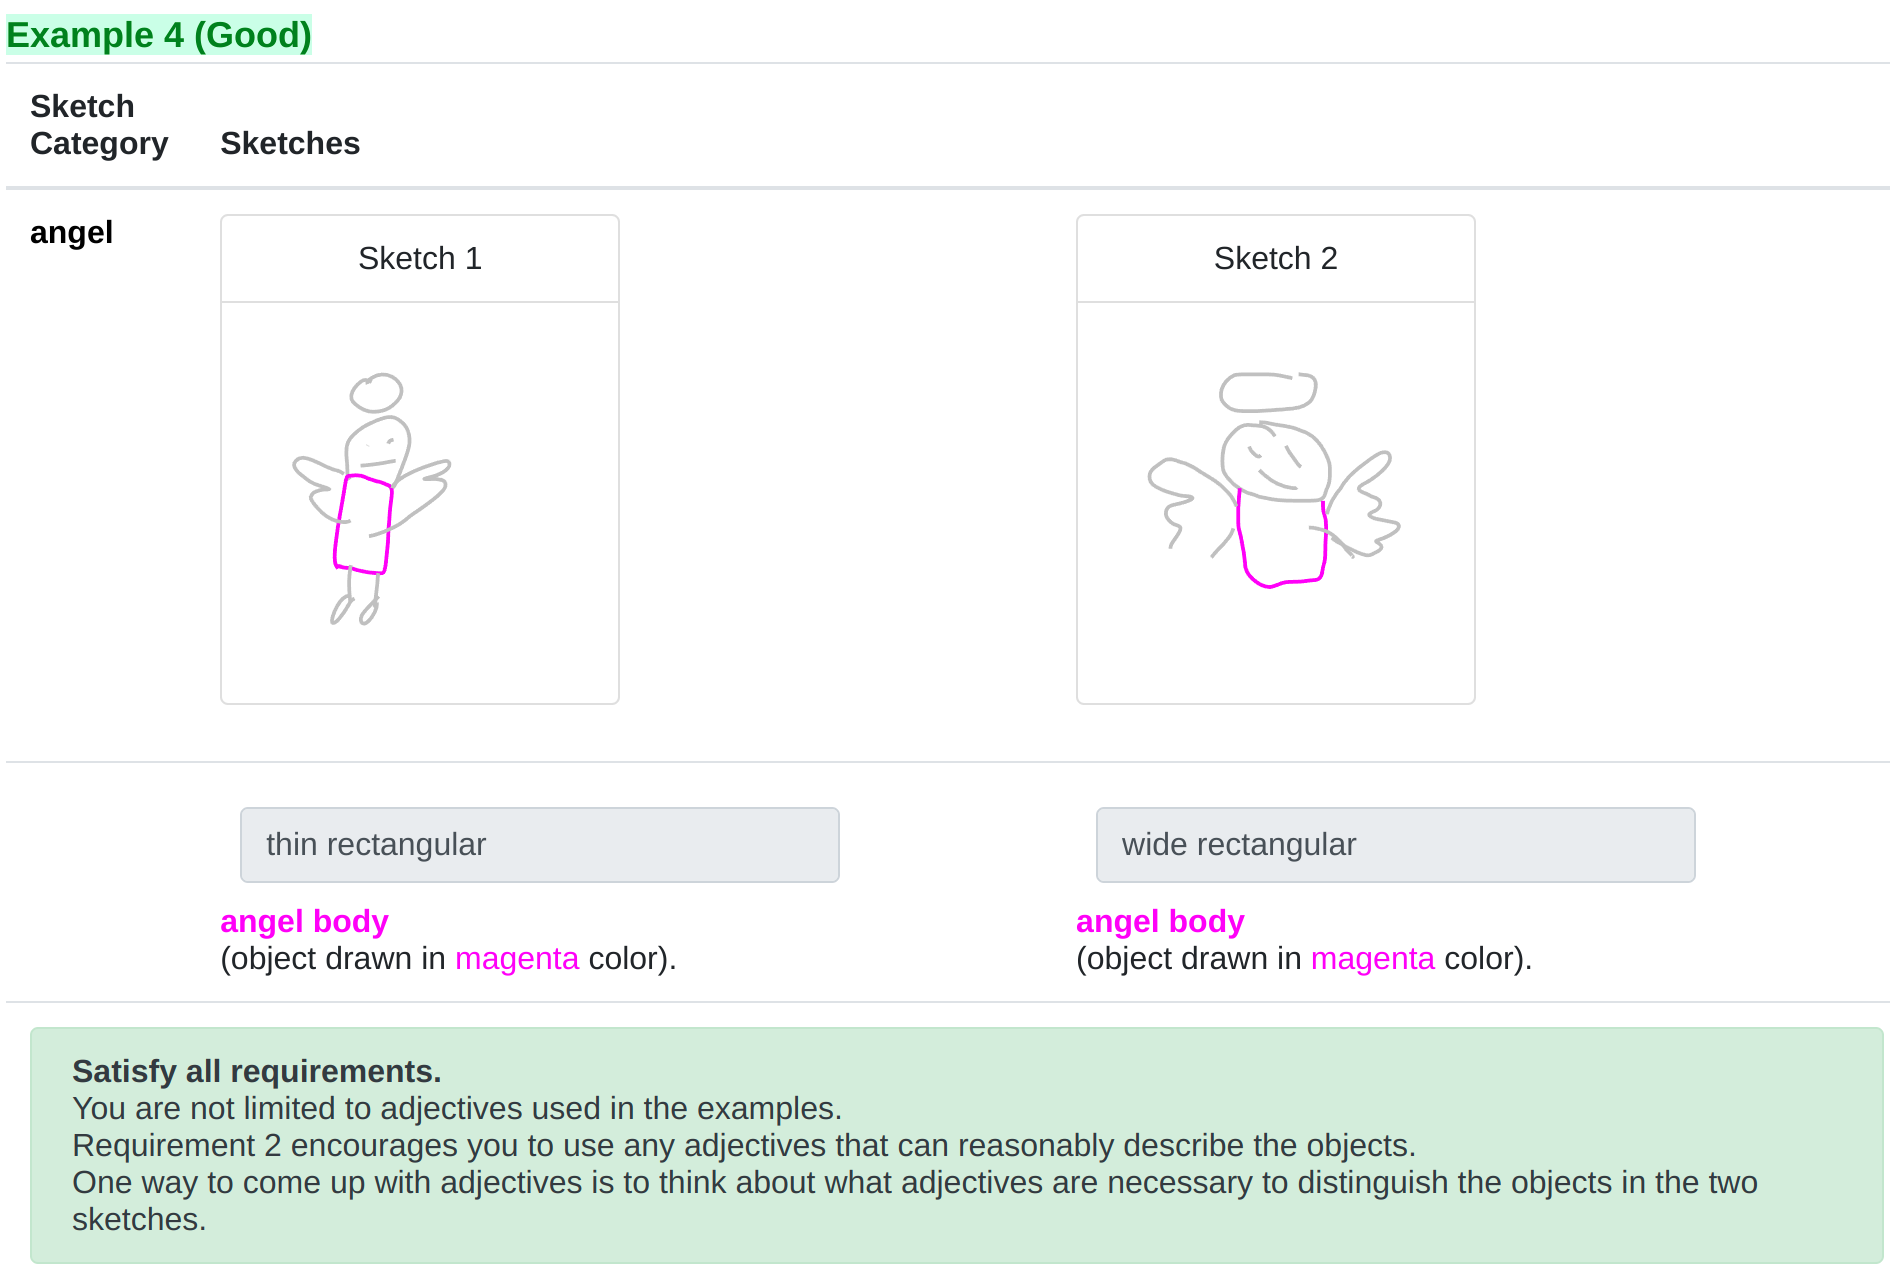
\includegraphics[width=0.8\linewidth]{data_collection/version2/v2example1.png}  
\end{subfigure}
\caption{2 examples used in the instructions to collect the contrasting sketch text dataset (Section \ref{datav2}).}
\label{v2.examples}
\end{figure*}

We relied on the examples in the instruction to give annotators an idea of what descriptions we wanted. 
Some examples that we used in the tasks are shown in Figure \ref{v2.examples}.
However, the downside was that, primed by the examples, annotators described the parts using words in the examples instead of coming up with a variety of descriptors, and we observed this behavior in the pilots. 
Therefore, we emphasized an additional requirement that asked the annotators to not limit themselves to words in the examples, and they should use any words that could illustrate the parts well. 

% The requirement that was a bit challenging for people to understand was the one regarding
% \textit{Do not use adjectives related to personal opinions, such as random, good, messy, beautiful, and strage, that are hard to achieve consensus if others were to validate your answers}. 
Since in the future we want to use our dataset to learn models that can generate sketch parts from text descriptions, the text should pertain to visual properties of the parts, so we required that \textit{Do not use adjectives that fail to describe specific visual properties of the objects in the sketches}. 
A caveat was that some annotators might consider descriptions about emotions expressed in the sketches unrelated to visual properties, since they are abstract compared to words like \textit{rectangular} and \textit{large}. 
We wanted to collect annotations for face sketches, and parts like \textit{eyes} and \textit{mouth} can be \textit{smiley} or \textit{sad}, so we added that adjectives describing emotions were allowed. 

The requirements used in the final version is shown in Figure \ref{v2.requirement.1}.

\subsubsection{Qualification}
We prepared 10 qualification questions; all are yes/no questions.
We used the qualification test to train turkers to understand the requirements better. 
Each question had a hint that stated which requirement and examples were helpful for solving the question. The purpose of the qualification test was not to trick annotators but to ensure speed and quality of the annotation. 
We show one question from the qualification in Figure \ref{v2.qualification.1}. 
To see the full test, refer to: \url{https://erinzhang1998.github.io/portfolio/v2qual}. 
At the end, we recruited 88 annotators to work on our task. 

\begin{figure*}[!htb]
\centering
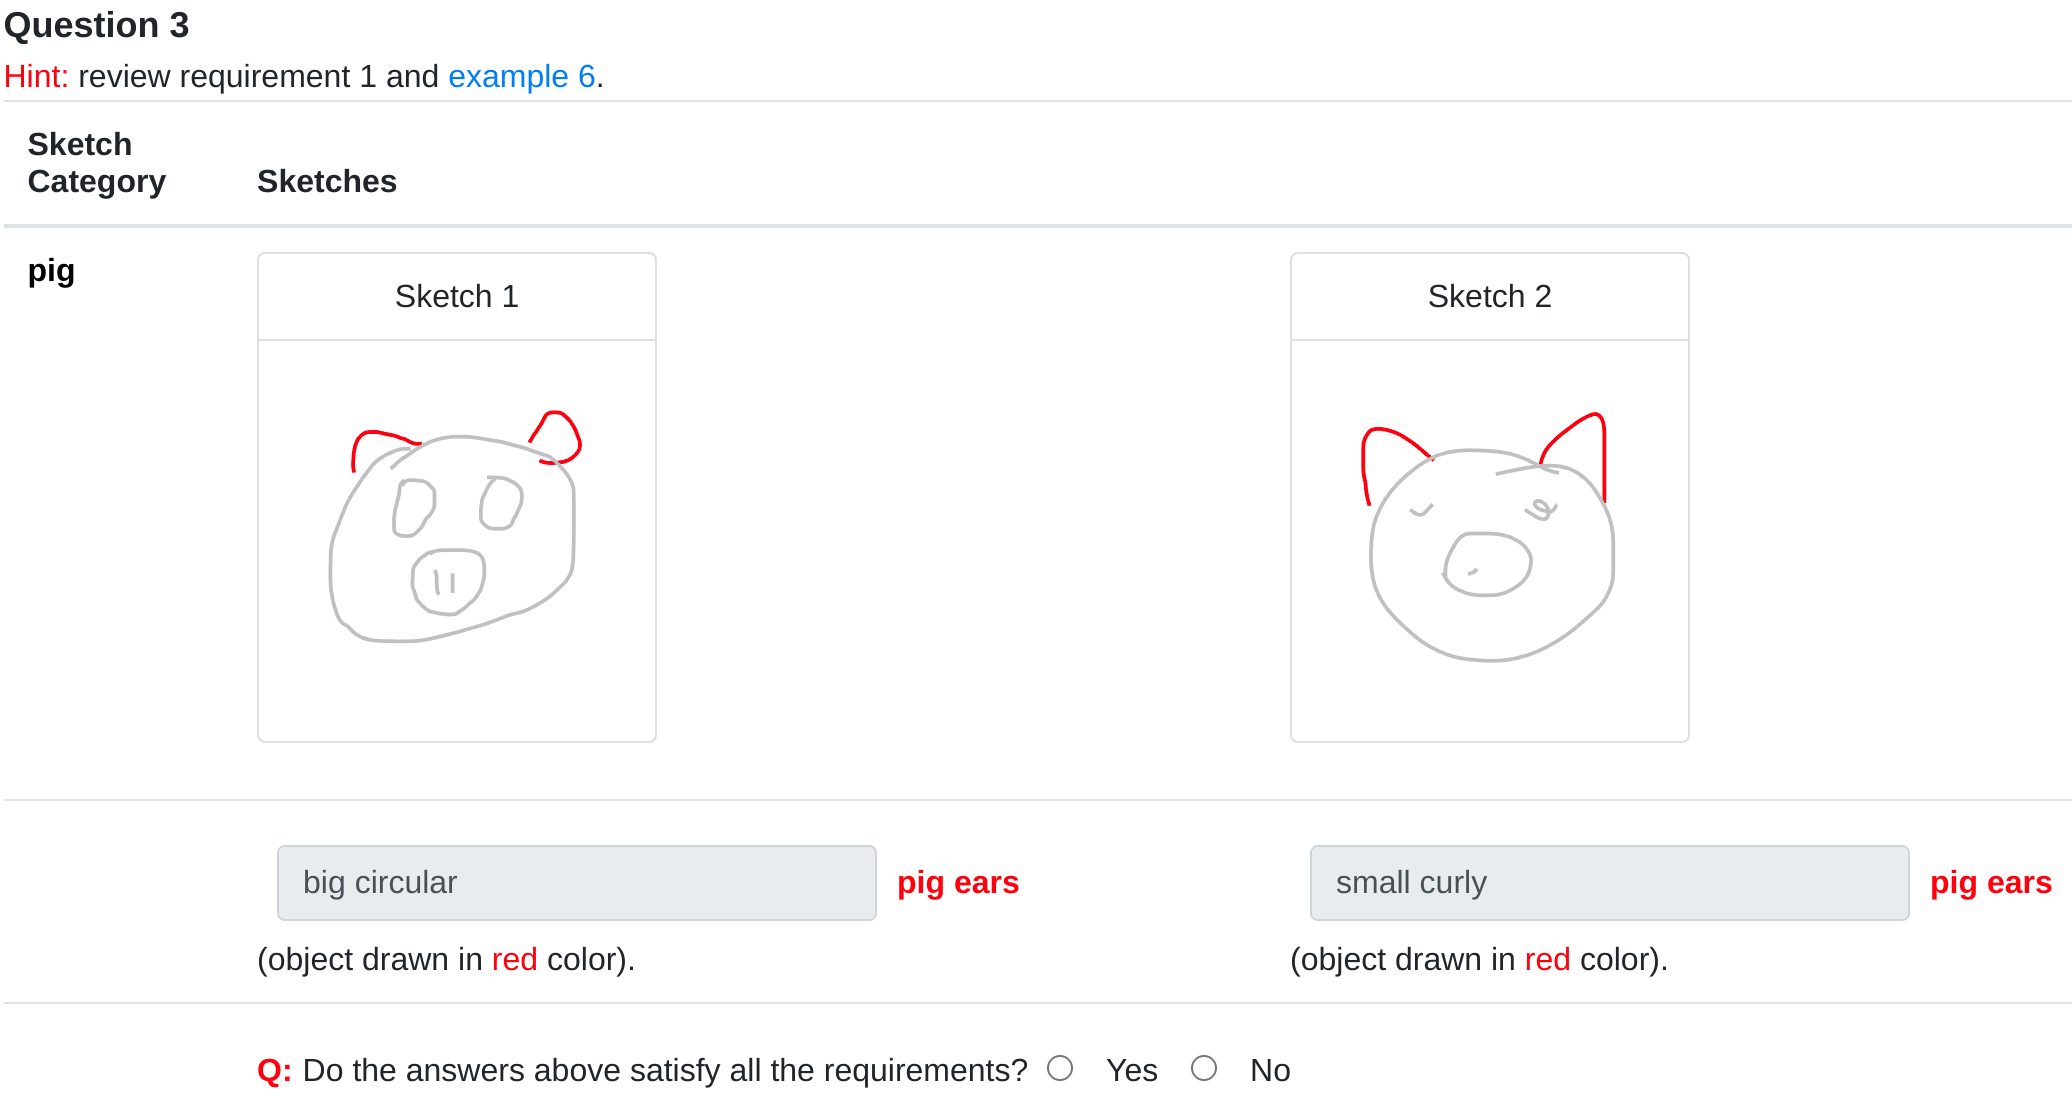
\includegraphics[width=\linewidth]{data_collection/version2/v2qualQ3.png}  
\caption{Question 3 from the qualification test used to collect the contrasting sketch text dataset (Section \ref{datav2}). We show a hint at the beginning of each question telling the annotators which requirement this question is testing. In this way, we encourage them to review the requirements so that they have a good understanding of the task and can provide high-quality annotations in the real HIT. The question interface is the same as main task interface that annotators will see when they annotate. The 1-to-1 mock-up helps them to be familiar with the workflow.}
\label{v2.qualification.1}
\end{figure*}

% \begin{table*}[!htb]
% \begin{minipage}[b]{1\textwidth}
% \centering
% \begin{tabular}{l|rrrrrrrrrr}
% \toprule
% Question Number  & 1 & 2 & 2 & 2 & 2 & 2 & 2 & 2 & 2 & 2  \\
% Correct Rate  & 1 & 2 & 2 & 2 & 2 & 2 & 2 & 2 & 2 & 2\\
% \bottomrule
% \end{tabular}
% \caption{Success rate of each question in the qualification test}
% \label{v2.qualification.success_rate}
% \end{minipage}
% \end{table*}
% We released $n$ copies of qualifications, and $n_2$ annotators scored $90$ or higher. The average score for the entire test is $x$, and the rate of correct answer for each question is shown in Table \ref{v2.qualification.success_rate}. Before releasing the qualification, we have tested the test on 


% 
\subsection{Results}

\subsubsection{Pilot 1}
In order to work out the data collection process, we chose the angel category and try to manually examine the sketches and categorize them based on 


One purpose of the pilot is to estimate the amount of money that we need to spend for each task, and from Table \ref{v2.workertime}, we see that []
\begin{table*}[!htb]
\begin{minipage}[b]{1\textwidth}
\centering
\begin{tabular}{l|rrrrr}
\toprule
~ & Max. & Min. & Mean & Med. & Std. \\
\midrule
Feb 01 Pilot  & 1 & 2 & 2 & 2 & 2   \\
Feb 04 Pilot  & 1 & 2 & 2 & 2 & 2  \\
Feb 08 Pilot  & 1 & 2 & 2 & 2 & 2  \\
Official Collection  & 1 & 2 & 2 & 2 & 2  \\
\bottomrule
\end{tabular}
\caption{Comparing time statistics of pilot task}
\label{v2.workertime}
\end{minipage}
\end{table*}

For the data collection process, we decide to collect for the face category of the QuickDraw dataset, and the reason for it was mainly to echo the choice of many SOTA generative modeling works that are done on the CelebA dataset. It seems that face generation is quite a starting point for many of the generative modeling work. We have also surveyed some text-to-image synthesis methods that use datasets like (1) CUB dataset (2) MNIST (3) Omniglot. Several sketch datasets include the one from DoodlerGAN and SketchBirds. A lot of the datasets focus on one or two categories, so we decide to do the same to ensure that with our budge, we can collect a dataset that contains enough signal to train a generative ML model. 

Clustering the faces, we strive to present to the annotators pairs of faces that are distinct as possible in order help them to provide good annotations. It is easier for them to grasp and understand the features of the objects if two sketches are presented in a contrasting way. 



If we use CLIP to extract the visual features for the entire face sketch.



\section{Dataset Summary} \label{datasummary}
\section{Dataset Summary} \label{datasummary}
Our dataset contains sketches, their semantic part annotations, and descriptions for every part in a sketch. 
The sketches comes from the QuickDraw dataset \citep{ha2017neural}, and the semantic part annotations come from the SPG dataset \citep{spg_paper}; both datasets are explained in details in Section \ref{relatedWorkChapter}.

We annotated for 2 categories of sketches: face and angel. 
For angel sketches, we annotate for the parts \textit{halo}, \textit{eyes}, \textit{nose}, \textit{mouth}, \textit{body}, \textit{outline of face}, and \textit{wings}. 
For face sketches, we annotate for the parts \textit{eyes}, \textit{nose}, \textit{mouth}, \textit{hair}, \textit{outline of face}. 


\begin{table}[!htb]
\begin{minipage}{1\textwidth}
\begin{center}
{\small
\begin{tabular}{lrrr}
\toprule
~ & Face & Angel \\
\midrule
Number of contrasting pairs & 2515 & 3060 \\
Number of distinct words & 833 & 1107 \\
Number of sketches & 572 & 787 \\
\bottomrule
\end{tabular}}
\caption{Dataset statistics by category.}
\label{table:dataset_stats1}
\end{center}
\end{minipage}
\end{table}

\begin{table}[!htb]
\begin{minipage}{1\textwidth}
\begin{center}
{\small
\begin{tabular}{p{9em} | p{1.5em}p{1.5em}p{2em}p{1.5em}p{1.5em} | p{1.5em}p{1.5em}p{1.5em}p{2em}p{1.5em}p{1.5em}p{1.5em} }
\toprule
~ & \multicolumn{5}{c}{Face} & \multicolumn{7}{c}{Angel}\\
~ & eyes & nose & mouth & hair & face & halo & eyes & nose & mouth & face & body & wings  \\
\midrule
Number of sketches & 
334 & 572 & 572 & 104 & 572 &
558 & 114 & 8 & 80 & 732 & 781 & 779 \\
Number of distinct words & 
228 & 360 & 325 & 152 & 314 & 
365 & 112 & 21 & 88 & 379 & 425 & 534 \\
Number of contrasting pairs &
689 & 401 & 687 & 126 & 612 &
559 & 114 & 8 & 80 & 733 & 785 & 781 \\
\bottomrule
\end{tabular}}
\caption{Dataset statistics by sketch parts. The phrase \textit{contrasting pair} refers to a pair of sketches with contrasting features that are presented to the annotators for descriptions of their parts.}
\label{table:dataset_stats_byparts}
\end{center}
\end{minipage}
\end{table}

\begin{figure*}[!htb]
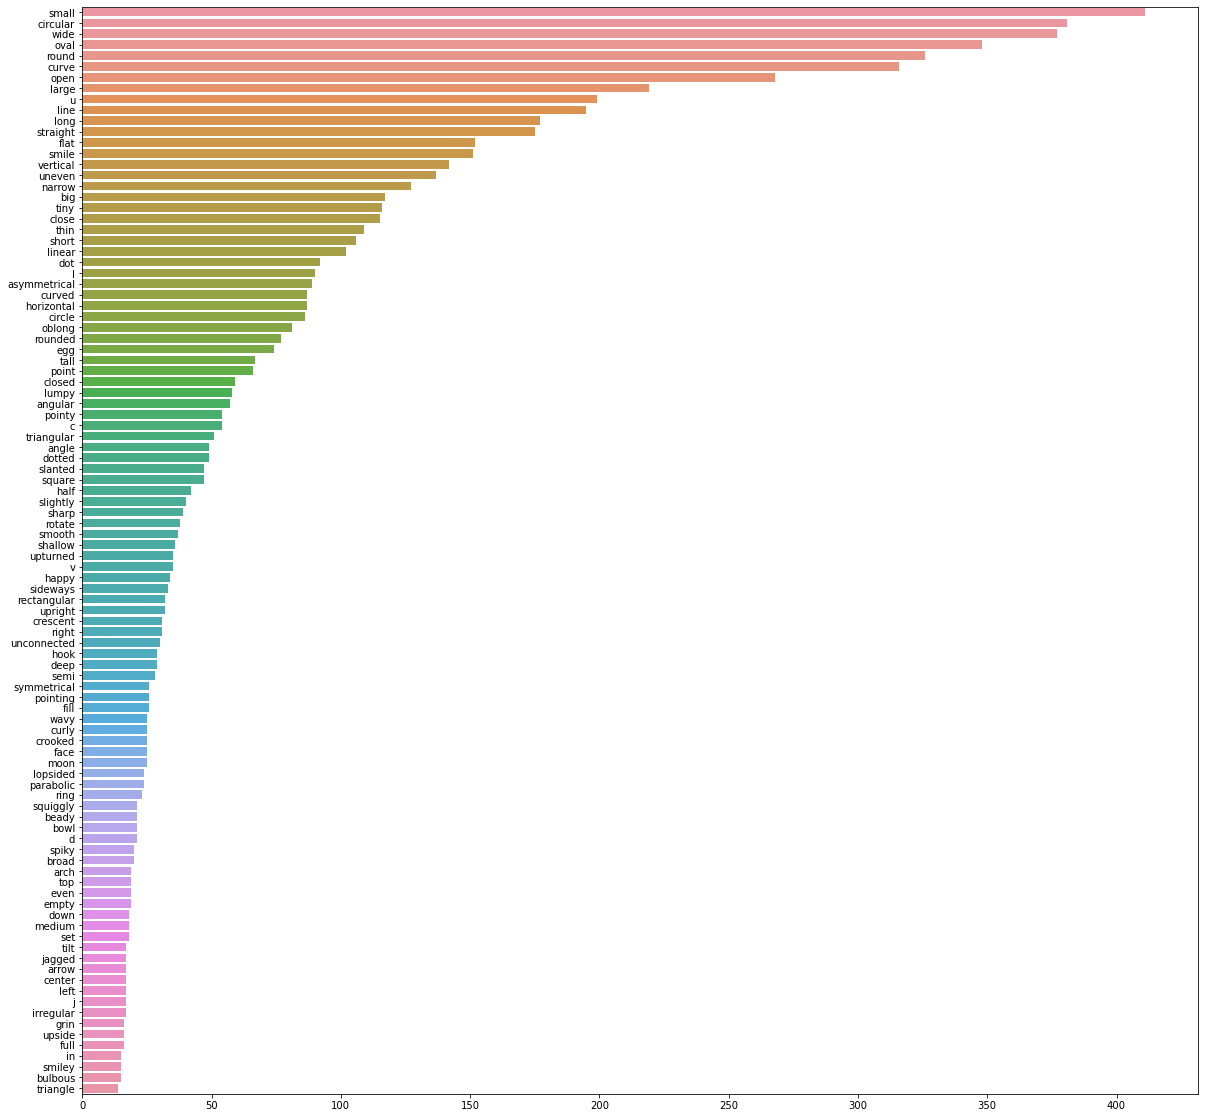
\includegraphics[width=\linewidth]{dataset_image/word_freq_face.png}  
\caption{Top 100 most frequent words in the dataset corpus.}
\label{word_freq}
\end{figure*}

In Table \ref{table:dataset_stats_byparts}, we present dataset statistics broken down by semantic parts, and, in Table \ref{table:dataset_stats1}, we show the same statistics by sketch category. In Figure \ref{word_freq}, we show 100 most frequently used words in our dataset. 

% \subsection{Compare with DoodlerGAN Dataset}
The \textit{Creative Birds} and \textit{Creative Creatures} datasets collected by DoodlerGAN \citep{doodlerGAN} contain 2 categories, like ours, but there are 9k sketches in each category, and ours contains one tenth as many. Although we fall short on the number of sketches and the variety of sketching styles, we approach creativity from a completely different angle: we focus on how people compose similar basic shapes to create sketches of different categories and adapt similar language to describe different sketch parts, as explained in Section \ref{introductionChapter} and Figure \ref{introduction.composition}.  

Our face sketches contain 5 different parts, and angel sketches has 7 parts; there are 7 parts in Creative Birds and 16 parts in Creative Creatures. Again, we do not annotate for as many parts as DoodlerGAN if compared directly with their dataset. However, in our dataset, every part in every sketch has at least 2 different language annotations describing the visual features, while DoodlerGAN has no language annotation. With text descriptions, in addition to part-based generative model, we can study how people compose concepts (e.g. \textit{large}$+$\textit{round}) and apply the same concepts to different semantic parts (e.g. \textit{large round eyes} and \textit{large round halo}).     

% In general, we observe that compared to previous work that tend to have a fixed list of adjectives for each object parts, the descriptions in our dataset are free-form and non-constrainted. This characteristics is desirable and aligns with our goal to allow robot to collaborate smoothly with humans, since different people would describe the same things in very diverse ways. 

% \subsection{Compare with SketchCUB Dataset}
% SketchCUB contains both sketch and language annotations \citep{sketchbirds}. However, it predetermines 312 binary attributes 


\begin{table}[!htb]
\begin{minipage}{1\textwidth}
\begin{center}
{\small
\begin{tabular}{p{5em} | p{1.5em}p{1.5em}p{2em}p{1.5em}p{1.5em} | p{1.5em}p{1.5em}p{1.5em}p{2em}p{1.5em}p{1.5em}p{1.5em} }
\toprule
~ & \multicolumn{5}{c}{Face} & \multicolumn{7}{c}{Angel}\\
~ & eyes & nose & mouth & hair & face & halo & eyes & nose & mouth & face & body & wings  \\
\midrule
small & 192 & 143 & 65 & 2 & 9 & 150 & 53 & 8 & 25 & 202 & 64 & 47 \\
oval & 123 & 7 & 11 &   & 207 & 258 & 1 &   &   & 145 & 42 & 23 \\
circular & 164 & 12 & 11 & 2 & 192 & 80 & 14 & 1 & 2 & 276 & 10 & 11 \\
round & 175 & 18 & 2 & 1 & 130 & 91 & 8 &   &   & 268 & 22 & 45 \\
wide & 94 & 16 & 193 &   & 74 & 84 & 2 &   & 12 & 50 & 120 & 111 \\
open & 118 & 7 & 106 &   & 37 & 54 & 6 &   & 1 & 79 & 137 & 26 \\
large & 98 & 41 & 58 &   & 22 & 66 & 6 &   &   & 131 & 54 & 85 \\
curve & 23 & 52 & 221 & 3 & 17 & 18 & 9 & 1 & 27 & 10 & 58 & 101 \\
triangular & 9 & 20 & 9 & 2 & 11 & 10 &   &   &   & 14 & 294 & 42 \\
line & 92 & 27 & 56 & 19 & 1 & 15 & 22 & 3 & 14 & 3 & 93 & 9\\
\bottomrule
\end{tabular}}
\caption{This table shows how many times the top-10 most frequently used word in the dataset is used to describe different parts in face and angel sketches. For example, \textit{small} is used in 192 descriptions for eyes in face sketches, and it is used 150 times to describe angel halos. People use the same words differently depending on the sketching context.}
\label{table:parts_share_description}
\end{center}
\end{minipage}
\end{table}

We observe that face and angel sketches share 486 words in total, and for the 200 words that occur most frequently in the dataset (all used in at least 13 part descriptions), 182 are shared across the two categories. Therefore, we believe that the datasets would allow us to study how people use similar words when sketching different objects. Although we cannot conclude in this project, we have already found some examples of the meaning of descriptors varied across sketches, after examining a few words. Figure \ref{datasummary.spiky} shows an example. In this example, \textit{spiky} is used to mean either short hair in face sketches or pointy, edgy wings in angel sketches. Moreover, there is an implicit orientation change between the two categories of sketches: while \textit{spiky hair} implies ``spike'' in the vertical direction, the phrase, \textit{spiky wings}, implies jigsaws pointing out from the angel body, horizontally.   

\begin{figure*}[!htb]
\begin{subfigure}{.5\textwidth}
\centering
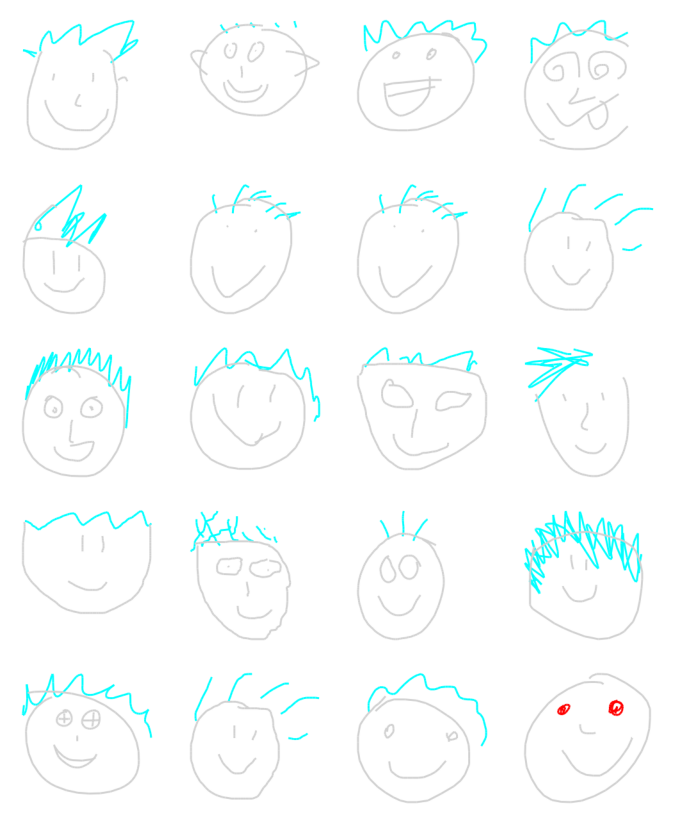
\includegraphics[width=0.9\linewidth]{data_collection/summary/spikyface.png}  
% \caption{Face sketches whose hair description contains the word \textit{spiky}. In this case, the word refers to short and coarse texture of hair.}
% \label{datasummary.spiky.face}
\end{subfigure}
\hspace{5mm}
\begin{subfigure}{.5\textwidth}
\centering
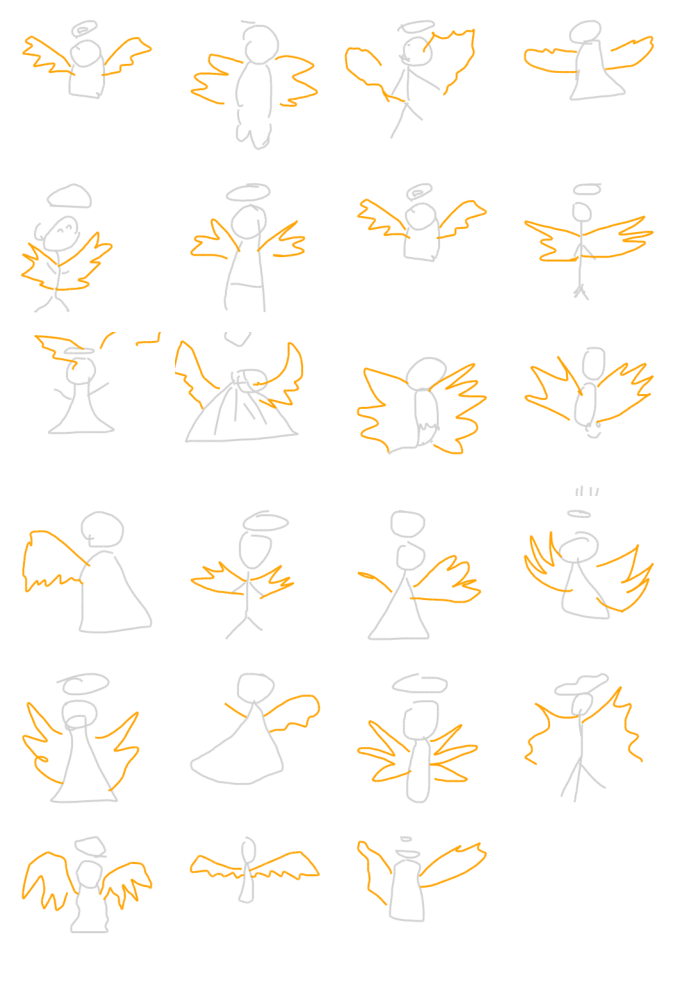
\includegraphics[width=\linewidth]{data_collection/summary/spikyangel.png}  
% \caption{Angel sketches whose wing description contains the word \textit{spiky}, which is used to represent the pointy edges on wings.}
% \label{datasummary.spiky.angel}
\end{subfigure}
\caption{Left: face sketches whose hair descriptions contain the word \textit{spiky}. In faces, the word refers to short and coarse texture of hair. Right: angel sketches whose wing description contains the word \textit{spiky}, which is used to represent the pointy edges on wings.}
\label{datasummary.spiky}
\end{figure*}

Moreover, 

\chapter{Modeling} \label{modelingChapter}
% In this chapter, we evaluate how 

\section{Task Definition} \label{modeling.task.def}
\begin{figure*}[!htb]
\begin{subfigure}{0.5\textwidth}
    \centering
    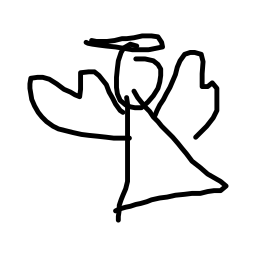
\includegraphics[width=0.5\linewidth]{modeling/angel340.png}
    \caption{$t_1$: \textit{wide triangular body}}
    \label{modeling.task.sketches.1}  
\end{subfigure}
\begin{subfigure}{0.5\textwidth}
    \centering
    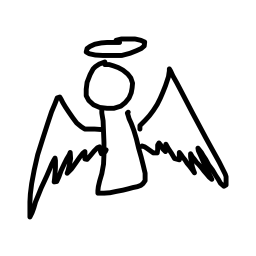
\includegraphics[width=0.5\linewidth]{modeling/angel389.png}   
    \caption{$t_2$: \textit{small rectangular body}}
    \label{modeling.task.sketches.2}  
\end{subfigure}
\caption{Two angel sketches, $s_1$ on the left and $s_2$ on the right, and their part annotations, $t_1$ and $t_2$. The task is for CLIP to determine which sketch matches a given $t_j$.}
\label{modeling.task.sketches}
\end{figure*}

% Since task should be method-independent, maybe mention that in this case we choose CLIP to do this task. This task can be done wtih any multimodal embeddings. 
Given two sketches $(s_1,s_2)$ and their part annotations $(t_1,t_2)$, such as the pair shown in Figure \ref{modeling.task.sketches}, the task is to determine which sketch $t_j$ should be paired with.
We use this task to evaluate the joint vision-language embedding space of CLIP, which is often used as part of the objective function for models that generate image from text; the objective function often involves maximizing the cosine similarity between the generated image and the provided text (or some variants engineered to work for the particular latent space of the generator used) \citep{clipDrawPaper,styleCLIPPaper,styleganNadaPaper,dalle2Paper}. 
Through this task, we can study how well CLIP can recognize different visual concepts in sketches, and the experiments can help us determine if CLIP can be used in similar ways to guide part-based sketch generation from language. Moreover, since we give CLIP the same pairs that were given to the annotators, we can learn if CLIP can understand how people are using language to describe the visual features of the sketches. 

We utilize CLIP to gain more insights into our dataset, beyond simple counting statistics. Given the nature of our dataset: a large variety of words but most words have very few occurrences, small number of images, text descriptions are contrastively collected by juxtaposing two images with opposite features, similar descriptions used for different purpose in different context. How does CLIP respond to this dataset, how well does CLIP embeddings align with our intuitions about these tasks? Specifically, for transferring the same word to be used in different context, or usage of words that are not the common meaning of words, how well can CLIP handle them, since it is trained on millions of images? Even though CLIP is not on the sketch domain, CLIP was trained on a large number of images on the internet, and there are GAN methods that have taken advantag eof CLIP embeddings to guide image generation: ClipDraw, StylCLIP, CLIP-NADA.      

\section{Task Definition}
Given two sketches $(s_1,s_2)$ and their part annotations $(t_1,t_2)$, determine which sketch $t_1$ should pair with, similarly for $t_2$. 
During data collection, we implicitly juxtapose two sketches, chosen to be as distinct as possible using some heuristic, either from different clusters or whose cosine distance is large, so the process of annotating the two dissimilar sketches is like the annotators are choosing the pair up one annotation with another. Implicitly, the annotators is pairing $s_1$ with $t_1$ and $s_2$ with $t_2$, so we would regard the ground truth pairing to be $(s_1,t_1)$ and $(s_2,t_2)$. We want to see how CLIP does on this task, if it is the annotator for the task, would it be able to generate the same pairing. Define cosine similarity to be.  

Given $(s_1,s_2)$, we use CLIP image encoder (zero-shot/fine-tuned) $f_v$ to extract visual features for the two sketches,  $f_v(s_1) \in {R}^{512}$, and $f_v(s_2) \in {R}^{512}$. We then use the zero-shot/fine-tuned CLIP text encoder to extract the text features for the part descriptions, namely we fill in the template $t = \texttt{[ADJ] [PART NAME]}$, where $\texttt{[ADJ]}$ is filled with the adjective phrases annotations, and $\texttt{[PART NAME]}$ is the name of the part in the sketches. For angels, $\texttt{[PART NAME]}$ is one of \textit{halo}, \textit{eyes}, \textit{nose}, \textit{mouth}, \textit{body}, \textit{outline of face}, \textit{wings}; for face, $\texttt{[PART NAME]}$ is one of \textit{eyes}, \textit{nose}, \textit{mouth}, \textit{hair}, \textit{outline of face}. After filling in the above template, we obtain the part annotations for the two sketches $t_1,t_2$.  
We obtain embeddings for the part annotations by encoding them through CLIP text encoder $f_t$: $f_t(t_1) \in {R}^{512}$, and $f_t(t_2) \in {R}^{512}$. We then calculate cosine similarity between all four pairs of $(f_v(s_i), f_t(t_j))$, $i,j \in [2]$, where consine similarity between two vectors $u,v$ is defined as $S_c(u,v) = \dfrac{u \cdot v}{\|u\| \|v\|}$. 
Therefore, given that our entire pipeline is $f$, $f(j) \in [2]$ output which of the two sketches $t_j$ will be paired with, and $$f(j) = \max_{i} S_c(f_v(s_i), f_t(t_j)) \hspace{2em} i \in [2]$$.    

\section{Metric}

Given $n$ pairs of two sketches and two part annotations, the same pairs that were provided by the annotators, we calculate an accuracy-like metric:
$$ acc = \frac{\sum_{k=1}^{n} \sum_{j=1}^2 \mathbbm{1}{(f(j) = j)}}{2n} $$

\section{CLIP Finetune}

We load the pretrained model from the \texttt{Python} \texttt{clip} package, specifically the \texttt{ViT-B/32} variant, which uses the Vision Transformer \citep{visiontransformer} as the image encoder; \texttt{B} stands for BERT Base model, and \texttt{32} stands for $32 \times 32$ input patch size. 

\subsection{Image Pre-Processing}
We use the data provided by SPG \citep{spg_paper}, which provides JSON files of the Quick,Draw! sketches in vector format: each sketch is composed of a sequence of $n$ strokes $S_i, i \in [n]$, and $S_i$ is a sequence of vectors $(\delta x,\delta y, p, l)$. $\delta x$ and $\delta y$ are changes in the $x,y$ coordinates with respect to the previous point; for the first point, it is with respect to $(25,25)$. All points are assumed to be drawn on a $256 \times 256$ canvas. $p=1$ if the point is the last point in the current stroke, and $p=0$ otherwise. The SPG dataset provides annotation for semantic segmentation of the sketches, so $l$ is a number representing the semantically meaningful object part.  

% We obtained the rendered sketches by using \texttt{Pycairo}, which is a Python module providing bindings for the cairo graphics library. We use a line width of $5$. After rendering, we manually examined the sketches and filter out face sketches that do not have a pair of eyes, a mouth and the face outline; we also filter out angel sketches that are incomplete or have all the parts merged together, possibly due to collection errors in SPG.   

\subsection{Text Pre-Processing}
We used the \texttt{spacy} package to preprocess the text. \texttt{spacy} provides trained natural language processing pipeline and includes models for, for example, token-to-vector and part-of-speech tagging. We use the \texttt{en\_core\_web\_sm} pipeline and its lemmatizer to reduce words to their basic forms. Moreover, we lower-case all words and remove punctuation, a list of which is provided by \texttt{Python} \texttt{string} package, \texttt{string.punctuation}. We also remove words like \textit{shaped}, \textit{sized}, \textit{and}, \textit{like}, since they act like stop words and do not provide additional visual descriptions of the sketches. Text descriptions are also tokenized by CLIP's tokenizer before passing into CLIP text encoder.     

\section{Loss Function}
During training, for a given batch size $b$, we have $b$ sketch-text pairs, $(s_k,t_k), k\in [b]$. We are essentially using classification over $b$ classes to finetune CLIP, using cross-entropy loss. With clip, we obtain image logits $X_v$ over the text descriptions and text logits $X_t$ over the sketches. The ground-truth, for both image and text, is 
$Y_v = Y_t = \begin{bmatrix}1 & 2 & \cdots & b \end{bmatrix}^T $ 

$$L(X_v, Y_v) = \dfrac{1}{b} \sum_{k=1}^b -\log\frac{\exp{{X_v}_{k,k}}}{ \sum_{c=1}^b \exp{{X_v}_{k,c}} } $$

And similarly defined for $(X_t, Y_t)$,
$$L(X_t, Y_t) = \dfrac{1}{b} \sum_{k=1}^b -\log\frac{\exp{{X_t}_{k,k}}}{ \sum_{c=1}^b \exp{{X_t}_{k,c}} } $$

The final loss is defined as:
$$L = \dfrac{1}{2} (L(X_v, Y_v) + L(X_t, Y_t))$$

\section{Data Augmentation}
As mentioned above, our dataset has a small number of sketches: 572 face sketches and 787 angel sketches.  

\chapter{Results \& Analysis} \label{analysisChapter}

\section{Classification Experiments}
In this set of experiments, what we do is that if we have a pair of sketches $(s_1,s_2)$, we use the CLIP image encoder (zero-shot/fine-tuned) $f_v$ to extract visual features $v_1$ and $v_2$ for the two sketches, where $v_1,v_2 \in \mathbb{R}^{512}$. We then use the zero-shot/fine-tuned CLIP text encoder to extract the text features for the part descriptions, namely we fill in the template $t = \texttt{[ADJ] [PART NAME]}$, where $\texttt{[ADJ]}$ is filled with the adjective phrases annotations, and $\texttt{[PART NAME]}$ is the name of the part in the sketches. For angels, $\texttt{[PART NAME]}$ is one of \textit{halo}, \textit{eyes}, \textit{nose}, \textit{mouth}, \textit{body}, \textit{outline of face}, \textit{wings}; for face, $\texttt{[PART NAME]}$ is one of \textit{eyes}, \textit{nose}, \textit{mouth}, \textit{hair}, \textit{outline of face}. After filling in the above template, we obtain the part annotations for the two sketches $t_1,t_2$.  
During data collection, we implicitly juxtapose two sketches, chosen to be as distinct as possible using some heuristic, either from different clusters or whose cosine distance is large, so the process of annotating the two dissimilar sketches is like the annotators are choosing the pair up one annotation with another. Implicitly, the annotators is pairing $s_1$ with $t_1$ and $s_2$ with $t_2$, so we would regard the ground truth pairing to be $(s_1,t_1)$ and $(s_2,t_2)$. We want to see how CLIP does on this task, if it is the annotator for the task, would it be able to generate the same pairing. Define cosine similarity to be        



% \begin{table}[htb!]
% \begin{minipage}{1\textwidth}
% \begin{center}
% {\small
% \begin{tabular}{lrrrr}
% \toprule
% & \multicolumn{2}{c}{Face} & \multicolumn{2}{c}{Angel}\\
% ~ & Test & Dev & Test & Dev \\
% \midrule
% zero-shot & 1 & 1 & 1 & 1 \\
% finetuned on face & 0.48 & 1 & 1 & 1 \\
% finetuned on angel & 1 & 1 & 1 & 1 \\
% finetuned on face $+$ angel & 1 & 1 & 1 & 1\\
% \bottomrule
% \end{tabular}}
% \caption{Statistics of CLIP}
% \label{clip_results_table.row_acc}
% \end{center}
% \end{minipage}
% \end{table}

\begin{table}[htb!]
\begin{minipage}{1\textwidth}
\begin{center}
{\small
\begin{tabular}{lrrrr}
\toprule
& \multicolumn{2}{c}{Face} & \multicolumn{2}{c}{Angel}\\
~ & Test & Dev & Test & Dev \\
\midrule
zero-shot & 0.54 & 0.55 & 0.56 & 0.57 \\
finetuned on face & 0.71 & 0.70 & 0.58 & 0.56 \\
finetuned on angel & 0.55 & 0.57 & 0.66 & 0.68 \\
finetuned on face $+$ angel & 0.71 & 0.69 & 0.68 & 0.68\\
\bottomrule
\end{tabular}}
\caption{Statistics of CLIP}
\label{clip_results_table.single_acc}
\end{center}
\end{minipage}
\end{table}


\chapter{Future Work} \label{futureChapter}
% The first question that we want to solve is what data should we collect in order to build a robot that can draw with humans? Inspired by drawing sessions created by Bob Ross, we have considered painting with robots and experimented briefly with oil painting on canvas with a Franka robot, but precise execution of brush strokes and the technical details surrounding manipulating brushes to create the desire scene are even very difficult for humans, and the focus of our research is to make a step towards human-robot collaboration on tasks, we do not want to be side-tracked by difficulties around robot control, which in itself is an extremely interesting problem that we wish to explore another time. 
\begin{figure*}[!htb]
\centering
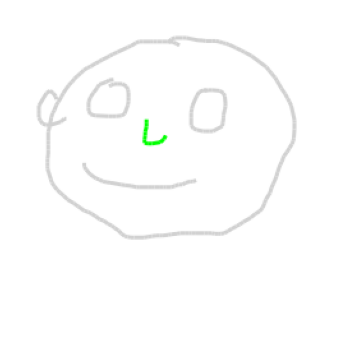
\includegraphics[width=0.3\linewidth]{future/future_nose_variety_392.png}  
\caption{.}
\label{results.hookNose}
\end{figure*}
There are many creative use of language in our dataset, and in follow-up work, we want to investigate what categories of creative usage are there and quantify how many cases are in each category. 
Most of our current characterization of the dataset are based on looking through a few examples in the datasets (there are a total of 11K!).
Since we did not put limits on what language annotators could use during data collection, such as specifying a fixed list of attributes for the annotators to choose from, the dataset contains a variety of ways of describing the same concept. For example, for a nose that looks similar to the one in Figure \ref{results.hookNose}, annotators describe it as \textit{hook-shaped}, \textit{c-shaped}, \textit{inverted j}, \textit{curved}, etc. We believe that this case is not the only one, and we want to quantify the diversity. In this way, we can evaluate how a multi-modal embedding space, such as the CLIP joint embedding, captures these relationships. Is the feature vector of the sketch collinear with the word features of every one of these words?          

So far, we have observed that face and angel sketches share many visual concepts. These could be related to length (\textit{long,short}), size (\textit{big,small}), geometry (\textit{circular, triangular}), direction (\textit{horizontal, vertical}), and many more. We want to evaluate more thoroughly which concepts are shared and which ones are unique to each category. In this way, we can understand better the chalenges around generalizing CLIP to unseen categories, indicated by results in Section \ref{results.acc}. 





\appendix
\chapter{Designing the Requirement Section for the Prompt-Guided Sketch Text Dataset} \label{appendixDataV1Req}
An excerpt from an old version of the instructions, in which we tried to explain a single \textit{step} of the annotation:
\begin{quotation}
In each task, we show \textbf{1 prompt} from which we would like to get
\begin{enumerate}
    \item A drawing containing 1 \textbf{entity} that you think illustrates the prompt.
    \item Text annotation for every \textbf{``component''} that makes up the entity.
    The word ``component'' is intentionally vague, and it depends on how you compose your drawing. For example, in the above example, the prompt is ``smiley face'', and during the process of creating a ``smiley face'' entity, we used 4 components: a face, a left eye, a right eye, and a mouth. For each component, you can annotate with ``face'', ``left eye'', ``right eye'', ``mouth'', respectively; you can also annotate with more details describing the shapes of each component: ``face that looks like an arc opening downwards'', ``a left eye that is an arc'', ``a right eye that looks exactly like the left eye'', ``an arc-like mouth''. Try to use creative and descriptive languages. You can draw a component using multiple strokes.
\end{enumerate}
\end{quotation}
We also need to come up with examples explaining each requirement. We select a few major sub-versions of the requirements resulted from circulating the interface within our lab.  

% Requirements and selected examples used in the first release in lab (Item 1 to 3 meant to enforce principal \ref{data_design_1}; Item 4 to 6 for \ref{data_design_2} and \ref{data_design_3}):
\begin{figure*}[!htb]
\begin{subfigure}{0.5\textwidth}
\centering
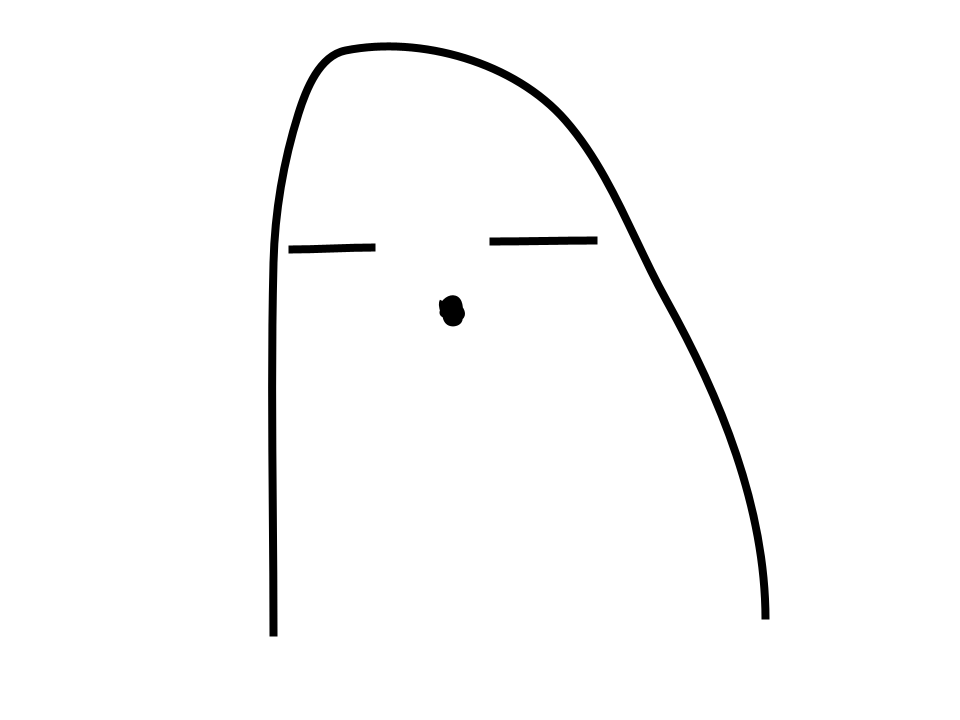
\includegraphics[width=.4\linewidth]{data_collection/host_amazon/hit_1/bad_smiley_face_ambiguous_face.png}  
\caption{An example included in the first version of the requirements, explained in more details in item \ref{v1_requirement1_3}.}
\label{v1.requirement_1.1}
\end{subfigure}
\end{figure*}

\begin{enumerate}
\item Do not draw entity that does not respond to the prompt. For example, given the prompt \textit{Smiley Face}, the drawing should not contain irrelevant objects like a house. 
\item Do not draw more than one entity that responds to the prompt. For example, One should not draw two \textit{Smiley Face} entities, although each \textit{Smiley Face} entity is good. However, you can draw multiple tree objects to illustarte the prompt \textit{Forest}.  
\item \label{v1_requirement1_3} Do not draw entity that is ambiguous in terms of illustrating the prompt. For example, the drawing (Figure \ref{v1.requirement_1.1}) looks more like a \textit{Sad Face} than \textit{Smiley Face}.
\item Do not draw one component that contains more information/content than what the annotation for that component describes. (A counterexample is illustrated in Figure \ref{v1.requirement_1.2}.)
\item Do not split the drawing of a component into multiple steps, unless you can annotate each step separately. (A counterexample is illustrated in Figure \ref{v1.requirement_1.3}.)
\item Do not annotate a component more than once.
\end{enumerate}



\begin{figure*}[!htb]
\ContinuedFloat
\begin{subfigure}{\textwidth}
    \centering
    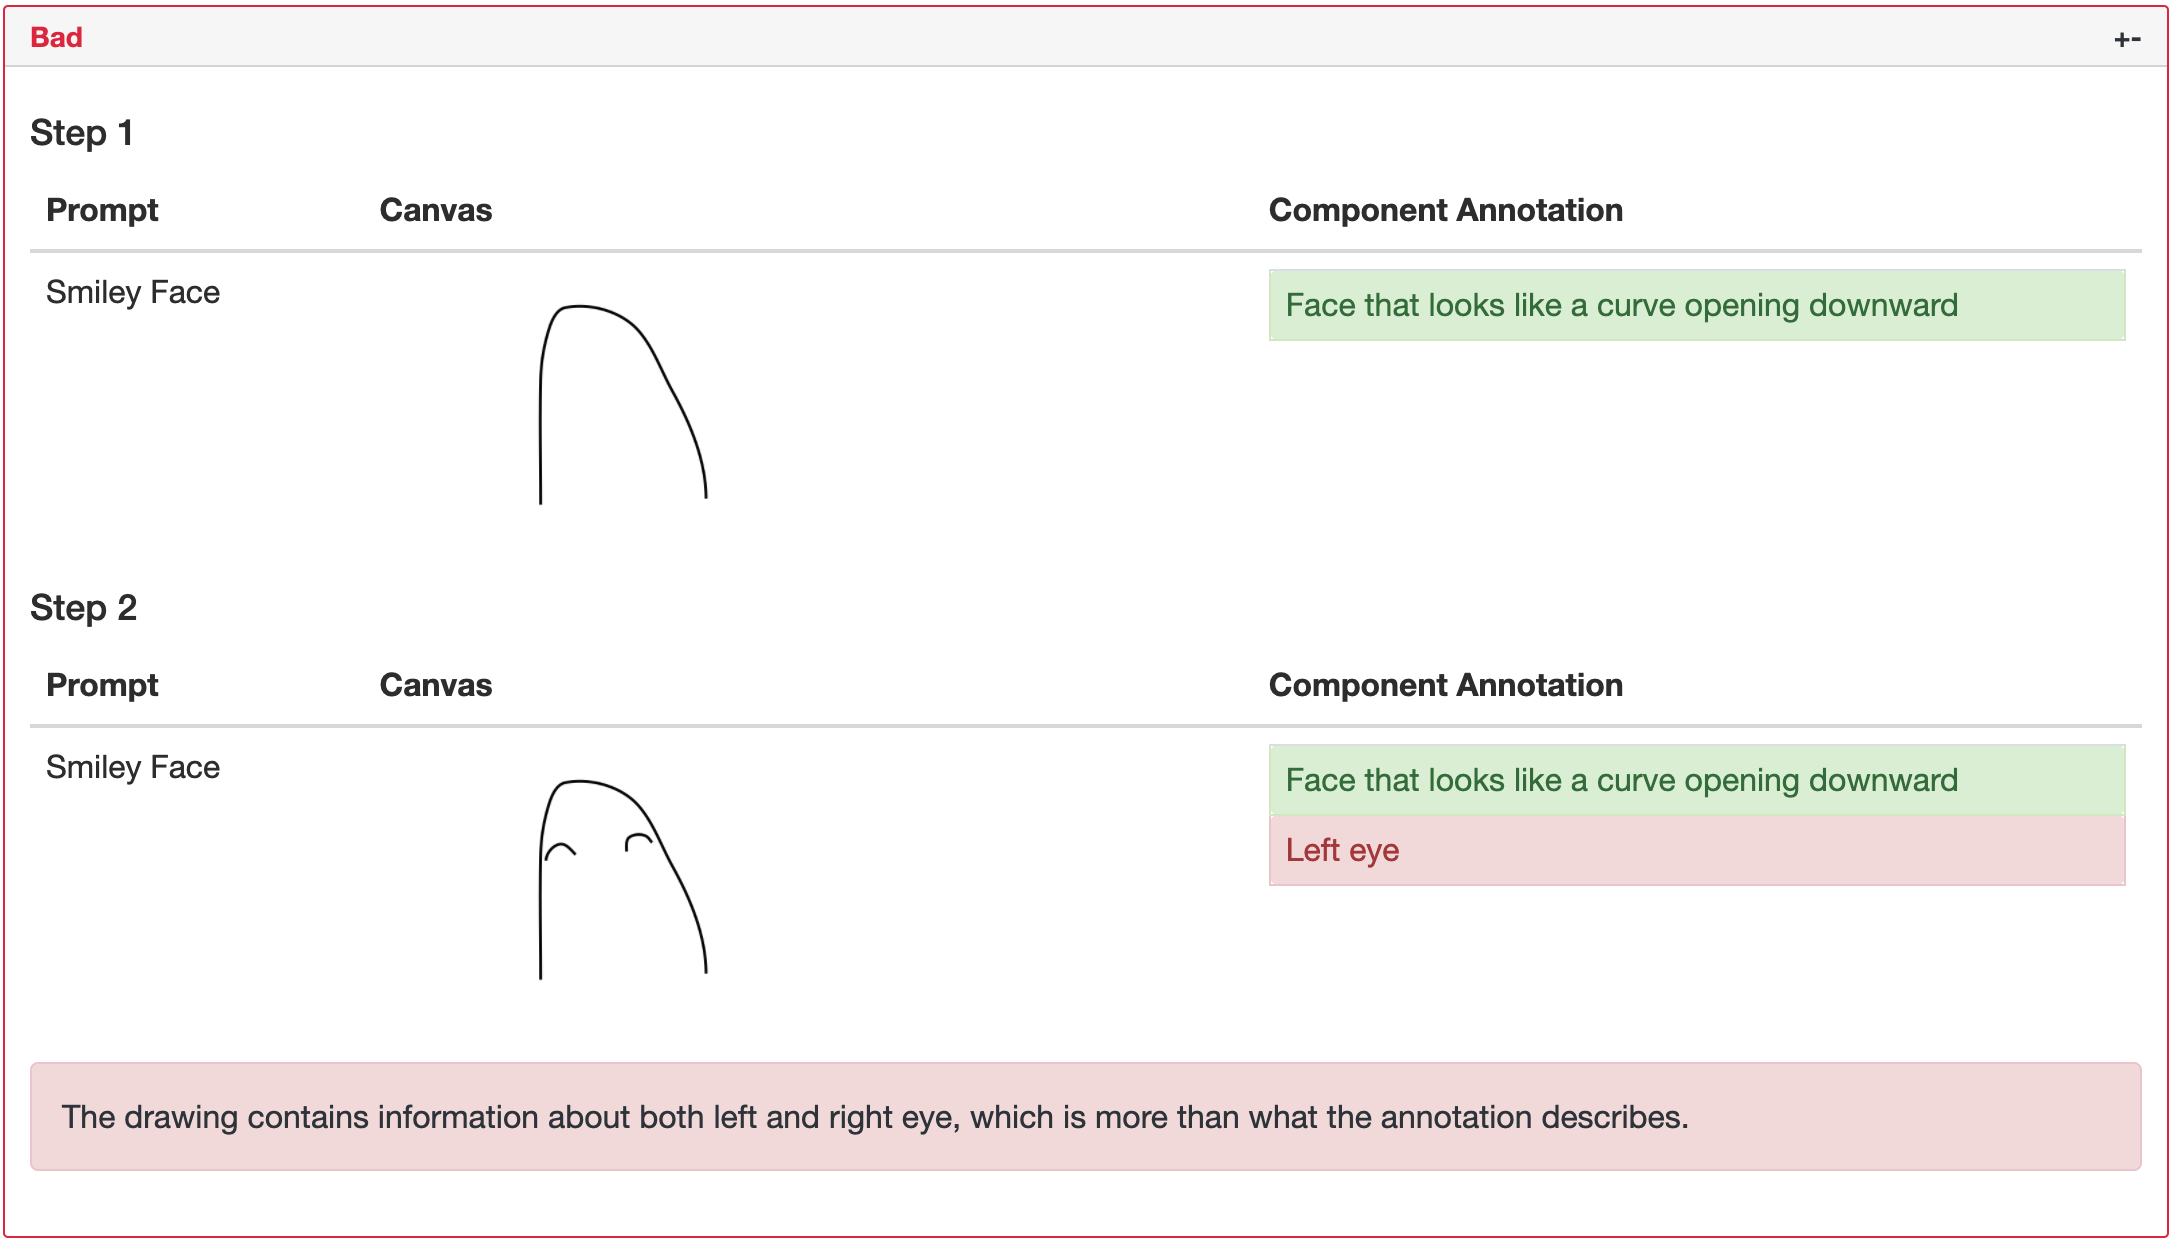
\includegraphics[width=.8\linewidth]{data_collection/v1_requirement1_bad1.png}  
    \caption{Unaligned drawing and text description.}
    \label{v1.requirement_1.2}
\end{subfigure}
\newline
\begin{subfigure}{\textwidth}
    \centering
    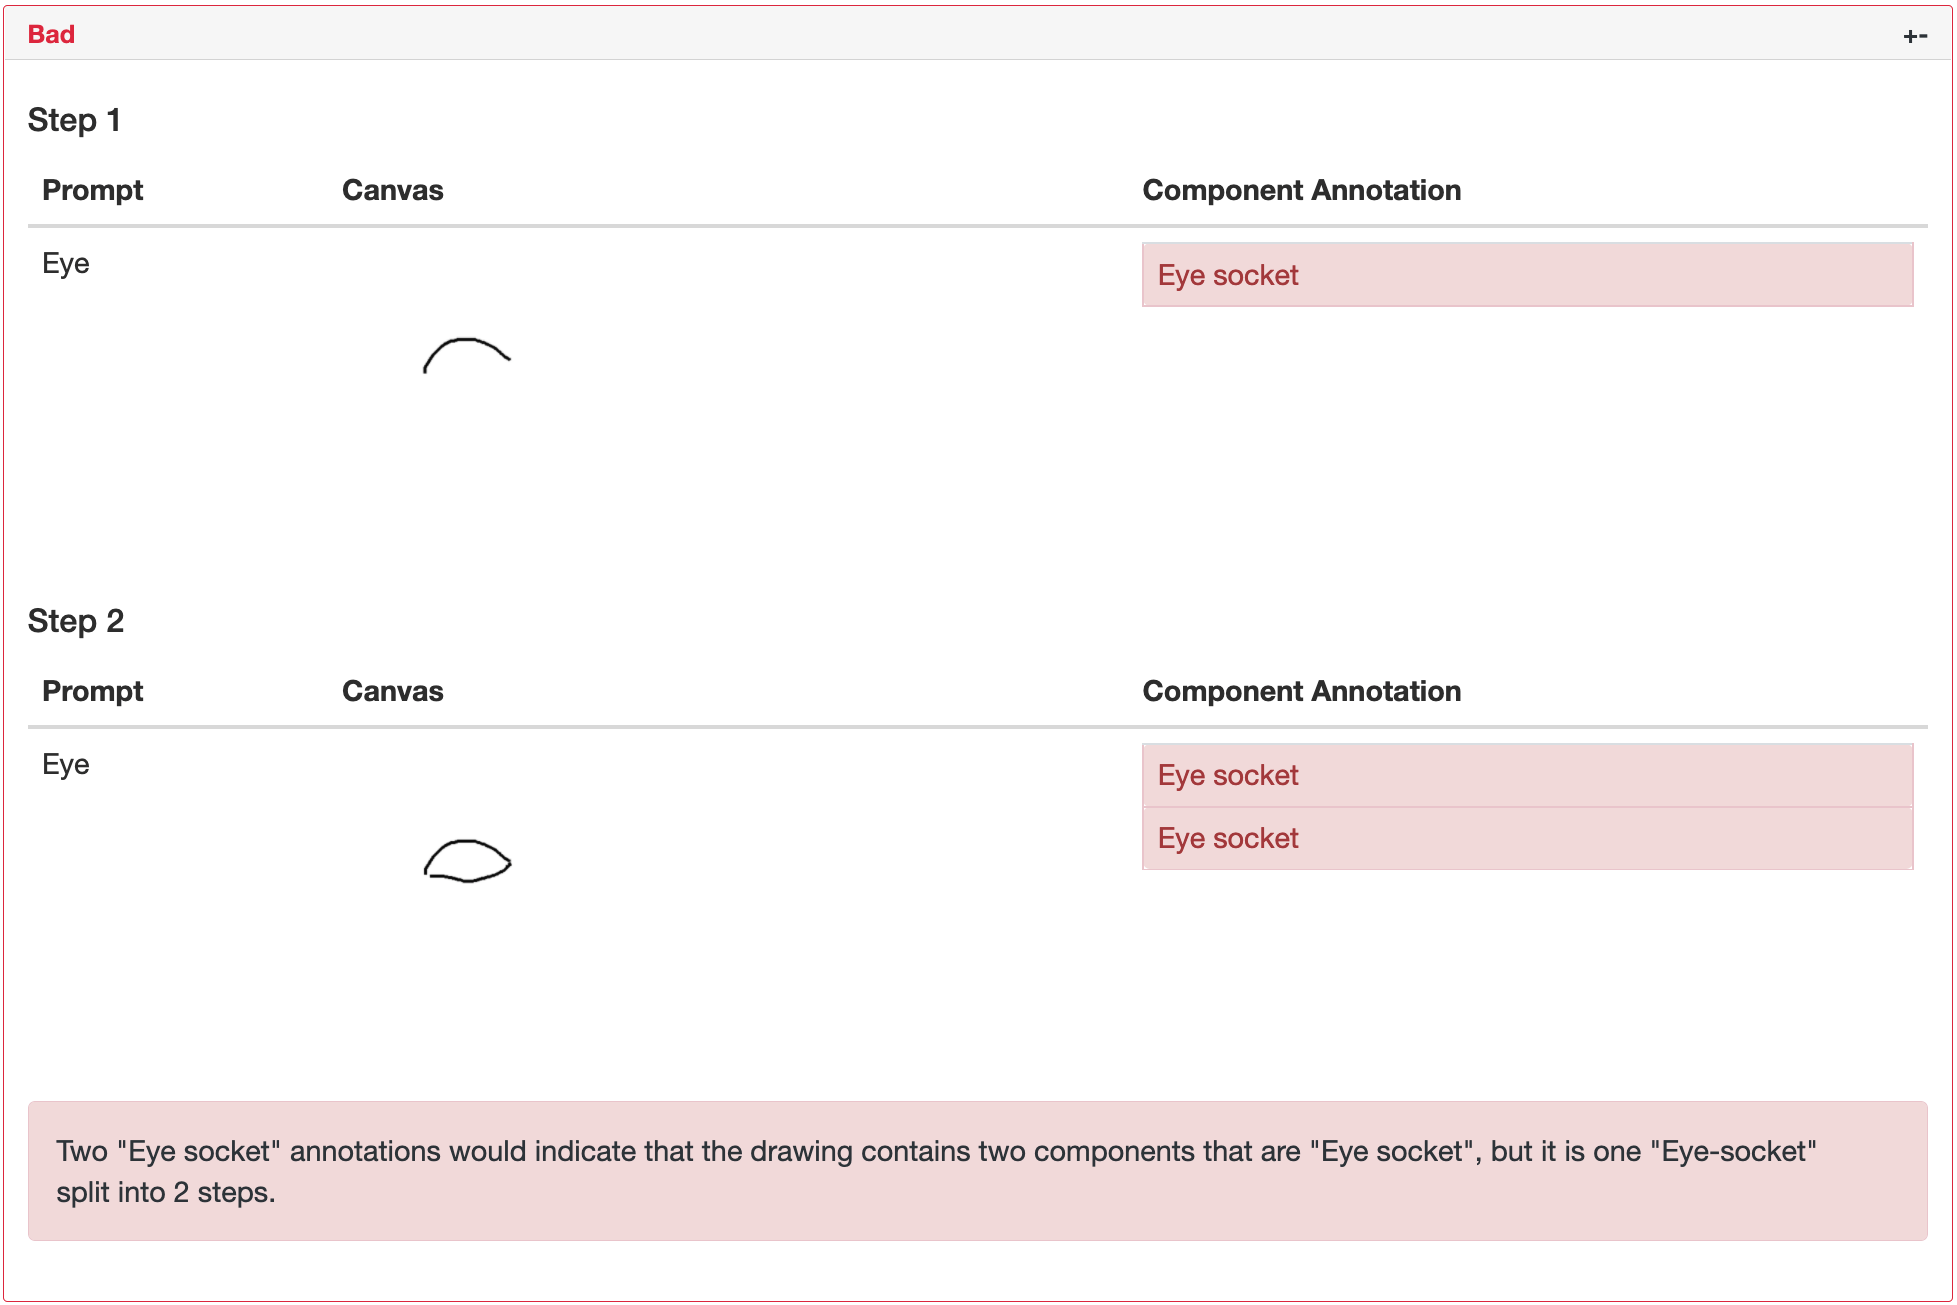
\includegraphics[width=.8\linewidth]{data_collection/v1_requirement1_bad2.png}  
    \caption{An example of misalignment: text description \textit{overflow} into multiple steps.}
    \label{v1.requirement_1.3}
\end{subfigure}
\caption{Screenshots of counterexamples used in first version of the requirements in Version 1.}
\label{v1.requirement_1}
\end{figure*}
% Figure 3x.a and 3x.b show some previous versions of the requirements. We eventually decided that  

% There is even more effort that went into defining the requirements of the task. This is really the section that we want to use to enforce all the DQ's. The final set of instructions is displayed in Figure x4.
% [Figure x4: final requirements]

% Comparing examples in requirements format:

% Methods to help understand the requirements. 
% Specifying which examples demonstrate which requirements, add next to the questions which requirement the question is testing. 

% Requirements and selected examples used in the second release in lab (Item 4 is meant to enforce principal \ref{data_design_1}; the other items for \ref{data_design_2} and \ref{data_design_3}):
\begin{enumerate}
\item Draw \textit{one} item at a time and provide its corresponding annotation. For example, the text annotation says ``left eye'', but two items are drawn: a left eye and a right eye.
\item The annotation should describe its corresponding item in the drawing \textit{entirely}.
\item The annotation should name the item.
\item Desired properties of good drawings:
\begin{itemize}
    \item Contain as many items as possible, but be sure that they all contribute to illustrating the prompt. For example, draw more than just two eyes for a face.
    \item Use shapes creatively. For example, draw a triangle for the left eye, and annotate accordingly with ``triangular left eye that shows suspicion''.
\end{itemize}
\item Desired properties of good annotations:
\begin{itemize}
    \item Use descriptive languages. For example, ``a left eye that looks an arc facing downward''.
    \item Include the intention/purpose of drawing an item. Explain in the annotation reasons for drawing the item. For example, ``thumbs-up next to the face that really shows how happy the face is''.
\end{itemize}
\end{enumerate}

% Requirements and selected examples used in the third release in lab (Item 1 is meant to enforce principal \ref{data_design_1}; the other items for \ref{data_design_2} and \ref{data_design_3}):
\begin{enumerate}
\item Each drawing should contain at least 2 steps.
\item Annotation of each step should include at least the name of the drawn object(s).
\item If draw multiple copies of the same object, draw each object in a separate step and give different annotations by using, for example, cardinal or ordinal numbers. (An example shown in Figure \ref{v1.requirement_3})
\item Differentiate between plural and singular forms.
\item The name of the whole should not be used for its parts. (An example shown in Figure \ref{v1.requirement_3})
\item The word "right" always refers to this side: $\Longrightarrow$
\end{enumerate}

\begin{figure*}[!htb]
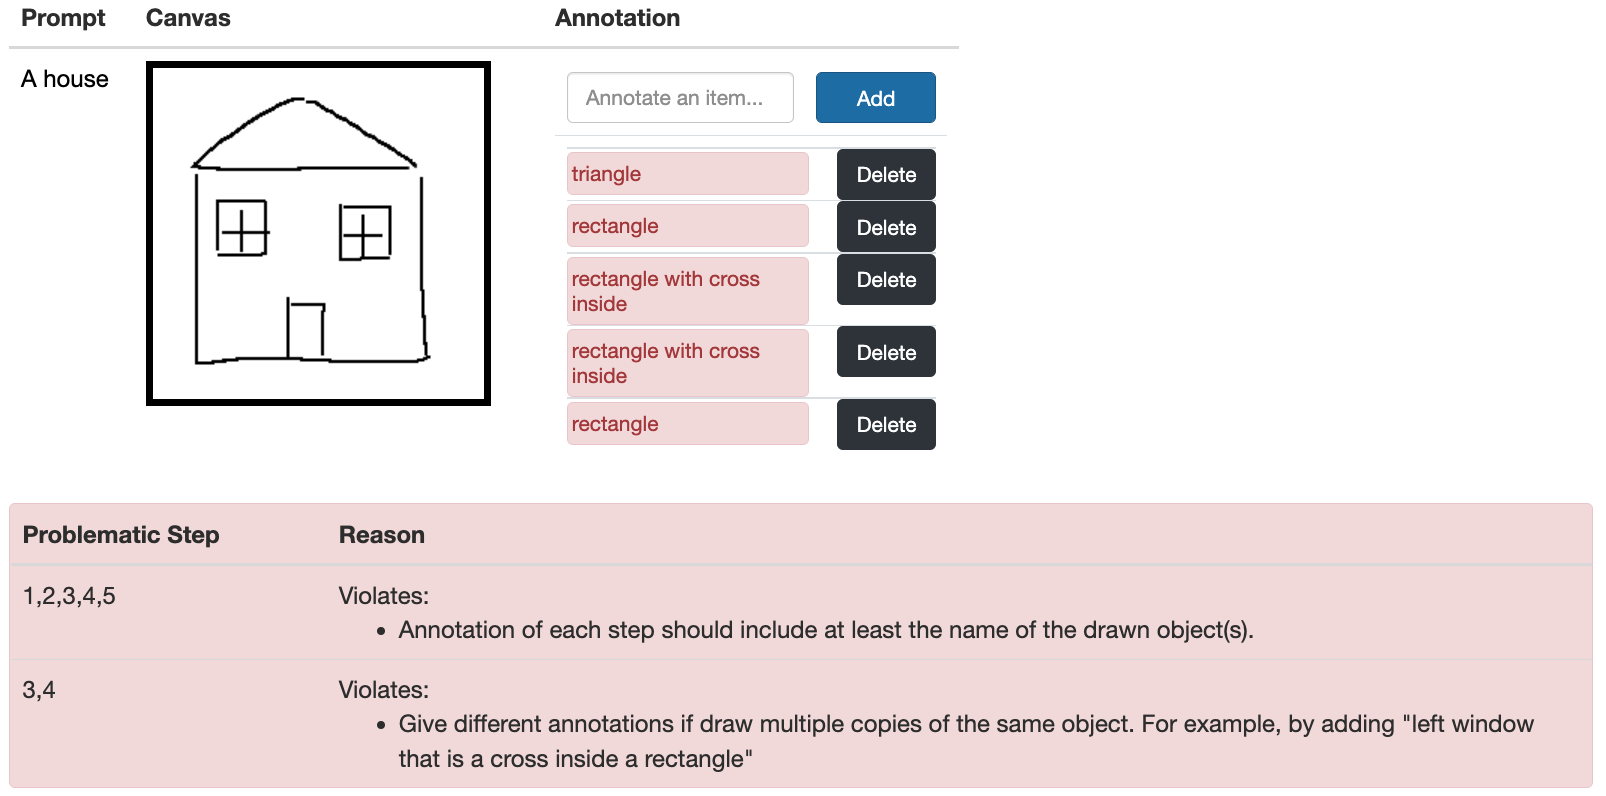
\includegraphics[width=.8\linewidth]{data_collection/v1_requirement3_bad1.png}  
\caption{Screenshots of counterexamples used in third version of the requirements.}
\label{v1.requirement_3}
\end{figure*}






\renewcommand{\bibname}{Bibliography}
\bibliographystyle{apacite}
\bibliography{thesiscite}
\end{document}
